\begin{savequote}[8cm]
\end{savequote}

\chapter{\label{ch:5-KF-NDGArToy}Kalman Filter Reconstruction for ND-GAr}

\minitoc
\section{Introduction}

In this chapter we will describe a Kalman Filter algorithm developed for particle tracking in ND-GAr's TPC. As outlined in Sec. \ref{sec:DUNE-ND-GAr} ND-GAr's TPC design is heavily inspired by ALICE's and it will re-purpose its MWPC's for signal formation. ALICE is a nucleus-nucleus collision experiment, designed to study the physics of strongly interacting matter at extreme values of energy density and temperature. The gas TPC technology was chosen by the ALICE collaboration due to its robustness in providing charged-particle momentum measurements with good two-track separation, particle identification, and vertex determination, even at the extreme levels of occupancy reached in Pb-Pb collisions. A similar TPC, but relatively smaller, has been used by the STAR experiment at RHIC~\cite{STAR:2002eio}. Recently, ALICE has undergone a significant upgrade~\cite{ALICE:2023udb}, requiring new R\&D in all areas of particle reconstruction.

Given the similarities between the detectors a collaboration was developed with the tracking experts from the ALICE experiment. The tracking algorithm developed for ND-GAr can be described as a Kalman Filter application  for a homogeneous cylindrical gaseous TPC, which is based on and expands the track fitting algorithm developed by the ALICE experiment. Part of the code is directly taken from \texttt{AliExternalTrackParam}, the ALICE TPC Kalman Filter framework~\cite{aliroot, Belikov:1997ska, carminati2003simulation}. 

The Kalman Filter developed by the ALICE experiment for track formation and reconstruction can be considered the state of the art in the field~\cite{Ivanov:2003yr, Arslandok:2022dyb}, but it has some limitations which make its direct application to a neutrino experiment such as ND-GAr problematic. The parametrization used by the ALICE experiment's Kalman Filter is such that it can only follow tracks that describe at most a semicircle in the plane perpendicular to the magnetic field, introducing non-physical breaking points in the reconstruction. Using a simple mirror rotation operation, the new algorithm is capable of following the track indefinitely, especially in the case of low-energy, low-mass (i.e. low energy loss) particles which form several circular trajectories inside the detectors, also known as ``loopers''. The application of this novel technique is particularly relevant for a neutrino experiment detector such as ND-GAr, for which particles are relatively low energy and are produced in neutrino interactions on gas at random points in the TPC volume. While many points of contact exist with the ND-GAr-Lite \texttt{KF-Lite} algorithm such as the shared ALICE-inspired parametrization, several differences exist and the ND-GAr Kalman Filter code was developed mostly independently and treated as a separate project.

The testing of the algorithm proceeded in two stages, much like for the \texttt{KF-Lite} algorithm (see Chapter \ref{ch:4-KF-NDGArLite}). We first produced a modular toy Monte Carlo tool capable of generating and propagating arbitrary particle tracks in a simplified detector geometry. This tool, which will be referred to as \texttt{fastMCKalman}, has been used to develop and test the algorithm~\cite{fastMCKalman}. Much like the ND-GAr-Lite toy Monte-Carlo tool, \texttt{fastMCKalman} was conceived to be highly modular and allowed to test many features of the algorithm independently. Once the reconstruction algorithm was considered to be fully developed, it was applied to data generated using \texttt{GArSoft}, the ND-GAr software suite (see Sec. \ref{Sec:GArSoft_Lite}), and its performance was compared to the reconstruction already available for the detector. Finally, once the reconstruction improvements were demostrated, the algorithm was fully integrated in \texttt{GArSoft} and proved to behave identically to the independent software contained in \texttt{fastMCKalman}.

This Chapter will be organized as follows: in Sec. \ref{Sec:KalGAr} we describe the ND-GAr Kalman Filter, outlining the difference with the \texttt{KF-Lite} algorithm; in Sec. \ref{sec:fastMCKalman} we describe the \texttt{fastMCKalman} toy Monte Carlo tool; in Sec. \ref{Sec:GArSoft-GAr} we describe the components of \texttt{GArSoft} that are unique to ND-GAr, including its original reconstruction algorithm; in Sec. \ref{Sec:ToyMCStudy_GAr} we describe the testing done for the algorithm using \texttt{fastMCKalman}; in Sec. \ref{Sec:Garsoft_Implementation} we describe the implementation of the algorithm in \texttt{GArSoft}.


\section{The Kalman Filter applied to ND-GAr}
\label{Sec:KalGAr}
The Kalman Filter described in this section has been developed to be used in an homogeneous cylindrical gas TPC. Much of the algorithm is analogous to the one described for ND-GAr-Lite in Sec. \ref{Sec:KFLite}, as both have been based on the same original ALICE TPC Kalman Filter. However, the code which actualizes the ND-GAr algorithm was developed in the context of the \texttt{fastMCKalman} tool largely independently and used directly parts of the ALICE TPC Kalman Filter framework \texttt{AliExternalTrackParam}. The Kalman Filter algorithm was also described in a publication currently under peer-review \cite{Battisti:2024nqq}.

The coordinate system defined for the algorithm is the same as the one used for the \texttt{KF-Lite} algorithm. Simplifying the geometry of the gas TPC to that of a cylinder, the $z$ coordinate is its height and the $xy$ plane is its base, with the $x$ being the horizontal direction and $y$ being the vertical. We assume that an ideal magnetic field is applied along $z$ which is the drift direction. Deviations from the ideal mono-directional magnetic field lines can be simulated and be accounted for using the infrastructure available in \texttt{AliExternalTrackParam}, but were not implemented. The spatial information in the perpendicular $xy$ plane is taken to be given by detector elements disposed in radial layers on the two sides of the cylinder. 

The algorithm is evolved along the free parameter, $x$, and its state vector follows the same parametrization outlined in Eq. \ref{eq:state} for the \texttt{KF-Lite} algorithm. A visual representation of the coordinates is given in Fig.~\ref{fig:Detector_var}. The evolution of the state vector is divided into two steps: a rotation of the global coordinates to a local frame and a propagation along the helix trajectory. The rotation is applied in the $xy$ plane around the center of the TPC cylinder. The rotation angle $\alpha = \arctan (y/x)$ is defined so that the $x$ coordinate becomes the radial distance from the center of the TPC and the $y$ coordinate is $\sim 0$. After the rotation the state vector is moved along the trajectory using a propagator function, as described in Eq. \ref{eq:ev}. The propagator function used for this algorithm is identical to the one outlined in Eq. \ref{eq:func} but is applied in local rotated coordinates. The propagation matrix, $F_k$, is also similarly calculated to the \texttt{KF-Lite} algorithm, as the Taylor expansion coefficient $\partial f_k / \partial s_k$ described in Eqs. \ref{eq:jacobian} and \ref{eq:jacobian2}, with the exception of the $q/p_{\text{T}}$ term, which is treated separately.

In order to compute the momentum loss, $\Delta p_k$, at each trajectory point, the ionization energy loss, $-\textrm{d}E/\left(\rho\textrm{d}x\right)$ (where $\rho$ is the density of the material in $\text{g/cm}^3$), of the particle is evaluated using the standard Bethe-Bloch formula in Eq. \ref{eq:Bethe}. The differential energy loss, $-\textrm{d}E/\left(\rho\textrm{d}x\right)$, is calculated using the properties of the most abundant gas present in the gas mixture in standard conditions and then multiplied by the material's density to obtain a reasonable approximation of the $\textrm{d}E/\textrm{d}x$~\cite{STERNHEIMER1984261}. The total momentum loss between two steps is then calculated by numerical integration~\cite{Griffiths2010}. 

In the evaluation of $F_k$, the $q/p_{\text{T}}$ parameter is treated as if it were static. A correction term, $c_k$ is added to the $q/p_{\text{T}}$ diagonal element of the covariance matrix, $\widetilde{C}_k$, after the propagation step (see Eq. \ref{eq:eloss-factor}). Similarly, the multiple scattering is treated through the noise correction matrix, $Q_k$ outlined in Eq. \ref{eq:Q}, which is derived from the calculation of the scattering angle. 

Each step in the evolution of the Kalman Filter can potentially fail, in which case the algorithm is stopped. This can happen mainly in two scenarios: $\sin \phi$ can be calculated to be out of range, i.e. $|\sin \phi|>(1-10^{-7})$ or the particle can lose all its remaining energy. Once the Kalman Filter is stopped, the information for each of the reconstructed points is saved. Flags are used to preserve information on which of the reconstruction steps have been successful and which have failed. 

One inherent limitation exists in the propagator function in Eq.~\ref{eq:func}, specifically in the equation describing the evolution of $\sin \phi$. The formula can only be applied within the range of $\sin \phi \in [-1,1]$, which describes one semi-plane. For $|\sin \phi|\rightarrow1$ the uncertainty on the parameter tends to infinity and the operation is no longer well defined. In radial coordinates this coincides with the moment when the particle is moving parallel to a detector's radial layer and the radial direction of the propagation is inverted. In order to overcome this limitation and further evolve the Kalman Filter, one can apply a \enquote{mirror rotation} or reflection on the state vector~\cite{lay2003linear}. The mirror plane is the one perpendicular to the $xy$-plane,  which connects the coordinate frame's center (i.e. the center of the TPC) with the center of the circular motion of the particle. In the local coordinate frame the mirror rotation is linear and can be written as:
\begin{equation}\label{eq:mirror}
    \left\{
    \begin{aligned}
        &s_k^\textrm{M} = M s_k,\\
        &C_k^\textrm{M} = M C_k M^T,
    \end{aligned}
    \right.
    \;\; \textrm{where} \;\;
    M=\begin{bmatrix}
    1 & 0 & 0 & 0& 0 \\
    0 & 1 & 0 & 0& 0 \\
    0 & 0 & -1 & 0& 0 \\
    0 & 0 & 0 & -1& 0 \\
    0 & 0 & 0 & 0& -1 
    \end{bmatrix}.
\end{equation}
The angle $\alpha$, which defines the local coordinate frame, needs to be updated accordingly. This is done by finding the angle $\alpha_\textrm{C}$ corresponding to the mirror plane, and updating $\alpha$ as:
\begin{equation}
    \begin{aligned}
       \alpha _k^\textrm{M} &=\alpha_\textrm{C}-\Delta \alpha \\
                   &= \alpha_\textrm{C}-(\alpha_k-\alpha_\textrm{C}).
    \end{aligned}   
\end{equation} 
Finally, to update the $z$ position the angular displacement around the center of rotation is calculated as:
\begin{equation}
    \Delta \phi_C = 2\arcsin \left( \frac{\Delta_{xy}}{2r_k} \right),
\end{equation}
where $\Delta_{xy}$ is the distance between the two points in the $xy$ plane. From $\Delta \phi_C$, the correspondent circumference arch in the $xy$ plane, $a_{xy}$, can be found, and from it, the displacement in the drift direction, $\Delta z_k$, reads:
\begin{equation}
    \begin{aligned}
        \Delta z_k &= a_{xy} \cdot \tan{\lambda_k} \\
             &= \Delta \phi_C \cdot r_k \cdot \tan{\lambda_k} .
    \end{aligned}  
\end{equation}
Once all the mirror operations are complete the closest trajectory point is found and the Kalman Filter is further evolved from there. From this point on-wards we will refer to the Kalman Filter algorithm, not including the mirroring operation as the Basic Kalman Filter or \texttt{BKF}. We will refer to the full algorithm, which includes both the \texttt{BKF} and the mirroring operation as the Corrected Kalman Filter or \texttt{CKF}. A flow chart describing the algorithm is shown in Fig.~\ref{fig:Logic}.
\begin{figure}[t]
     \centering
     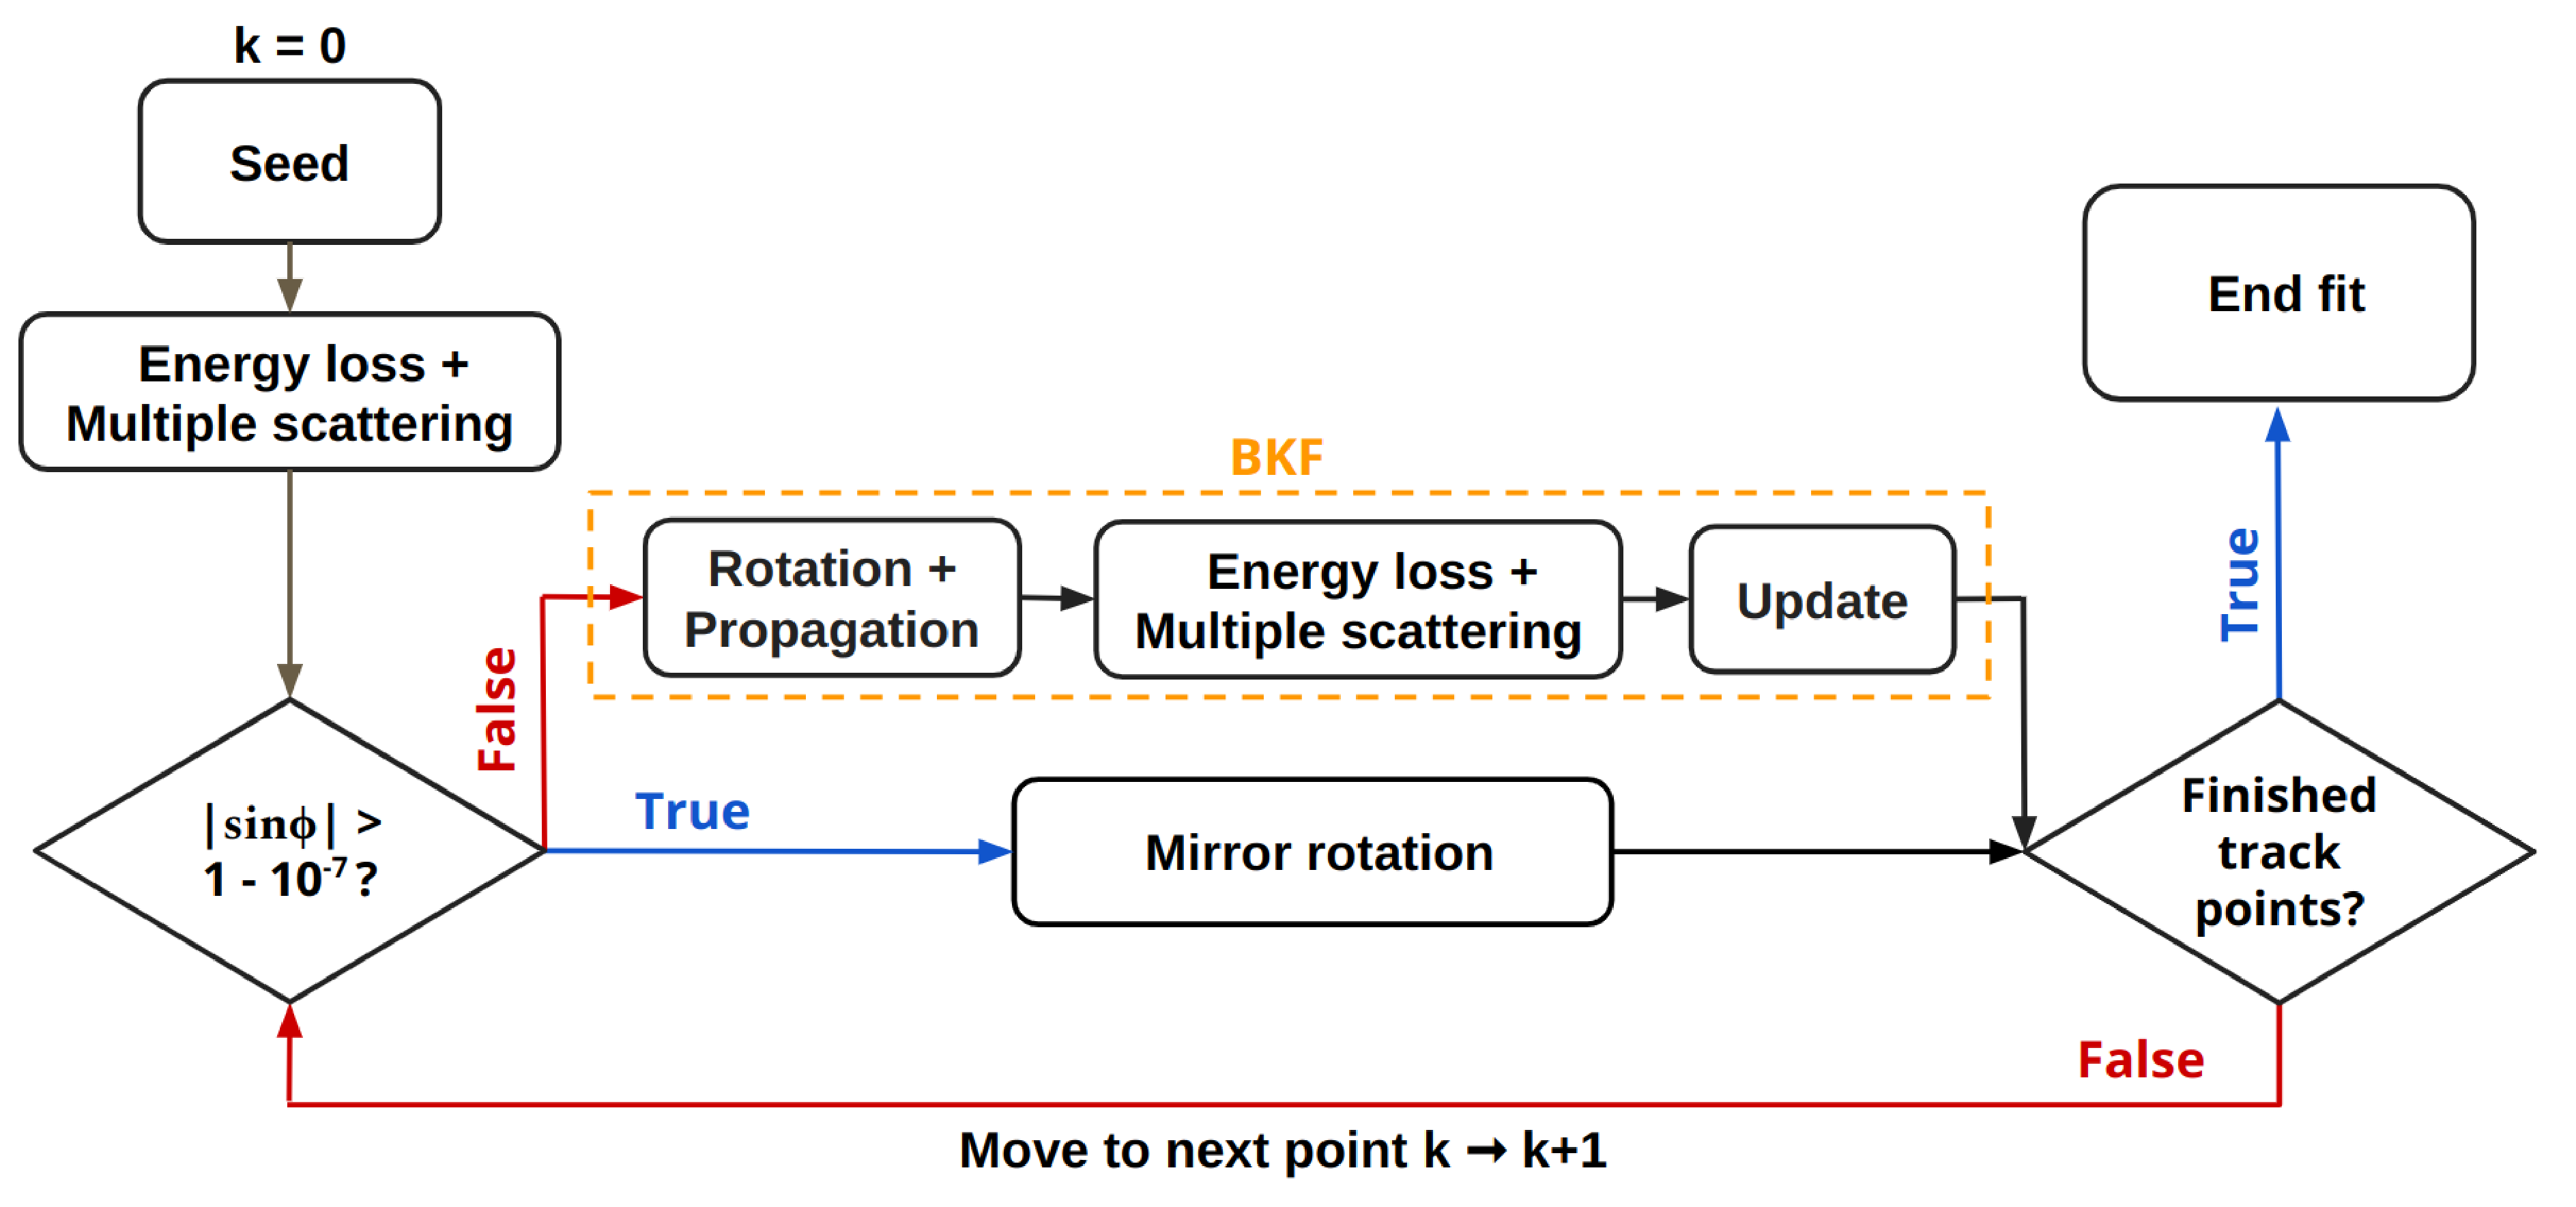
\includegraphics[width=\textwidth]{figures/ch5-KF_NDGAr/KFFlowChart_new.eps}
     \caption[Flow chart describing the \texttt{CKF} algorithm.]{Flow chart describing the \texttt{CKF} algorithm. A seeding algorithm is used to obtain an estimate for the status of the system at the start of the trajectory $k=0$. Energy loss and multiple scattering corrections are applied to the estimate. The fit is then moved to the next point $k\rightarrow k+1$ either by applying the the \texttt{BKF} procedure or by using the mirror rotation, in the case that the limits of the $\sin\phi$ range have been surpassed. The algorithm is iterated point by point until the end of the trajectory is reached. Other minor modifications have been made to the \texttt{CKF} algorithm compared to the \texttt{BKF} in order to make the mirroring operation more stable. }
        \label{fig:Logic}
\end{figure}


The seeding strategy used for the \texttt{CKF} (as well as for the \texttt{BKF}) consists in the simple three-point circle finding algorithm which was also used for the Kalman Filter algorithm developed for ND-GAr-Lite described in Sec. \ref{Sec:SeedingLite}. Similarly to what was done for the ND-GAr-Lite seeding algorithm, this will be referred to simply as \texttt{Seed}. The only notable difference between the two algorithms is that, while for the ND-GAr-Lite algorithm, only the diagonal elements of $C_0$ were calculated, in this case the off-diagonal terms are also considered. 

The \texttt{Seed} estimation for both the covariance matrix $C_0$ and the state vector $s_0$ is adjusted for energy loss and multiple scattering using the same method outlined the ND-GAr-Lite algorithm. The total distance traveled, needed to calculate total energy loss and the scattering angle $\theta_\texttt{M}$, is determined by summing the distances between the starting and midpoint, and the endpoint used for circle finding.

\section{The toy Monte Carlo simulation}
\label{sec:fastMCKalman}

To generate particle samples and validate the \texttt{CKF} algorithm, we developed a toy Monte Carlo (MC) tool called \texttt{fastMCKalman}~\cite{fastMCKalman}. This tool, stemming from the \texttt{AliExternalTrackParam} framework in the \texttt{AliRoot} code-base~\cite{aliroot}, was designed to be complemented by \texttt{RootInteractive}~\cite{RootInt}, an advanced statistical analysis tool. \texttt{fastMCKalman} has been developed with several objectives in mind: conducting rapid Monte Carlo (MC) simulations to evaluate tracking performance metrics, particle identification, and time-of-flight measurements across various detector setups. It was also designed to facilitate detailed studies on signal distortion in the ALICE detector and the derivation of performance metrics for its Run-3 upgrade and future iterations. 

The first step in the toy Monte Carlo simulation consists in defining a simplified detector geometry. The radius and length of the TPC cylinder are specified, together with the number of pad rows, the spatial resolution of the detector in the radial and drift directions (defined as $\sigma_{r\phi}$ and $\sigma_Z$ respectively) and the gas properties (i.e. the radiation length in cm, $X_0$, the density in g/cm$^3$, $\rho$, and the gas pressure in atm, $P_\textrm{gas}$). A diagram of the detector cylinder is shown in Fig.~\ref{fig:DetectorFastSim}. 

\begin{figure}[t]
     \centering
     % \begin{subfigure}[b]{0.48\textwidth}
     %     \centering
         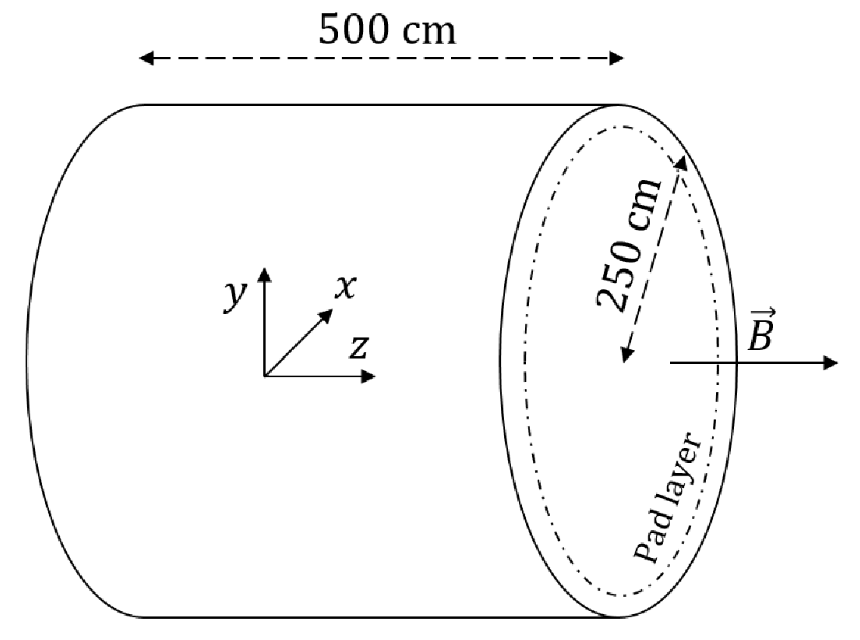
\includegraphics[width=0.6\textwidth]{figures/ch5-KF_NDGAr/Detector_diagram_new.png}
         % \caption{}
         % \label{fig:Detector}
     % \end{subfigure}
     % \begin{subfigure}[b]{0.48\textwidth}
     %     \centering
     %     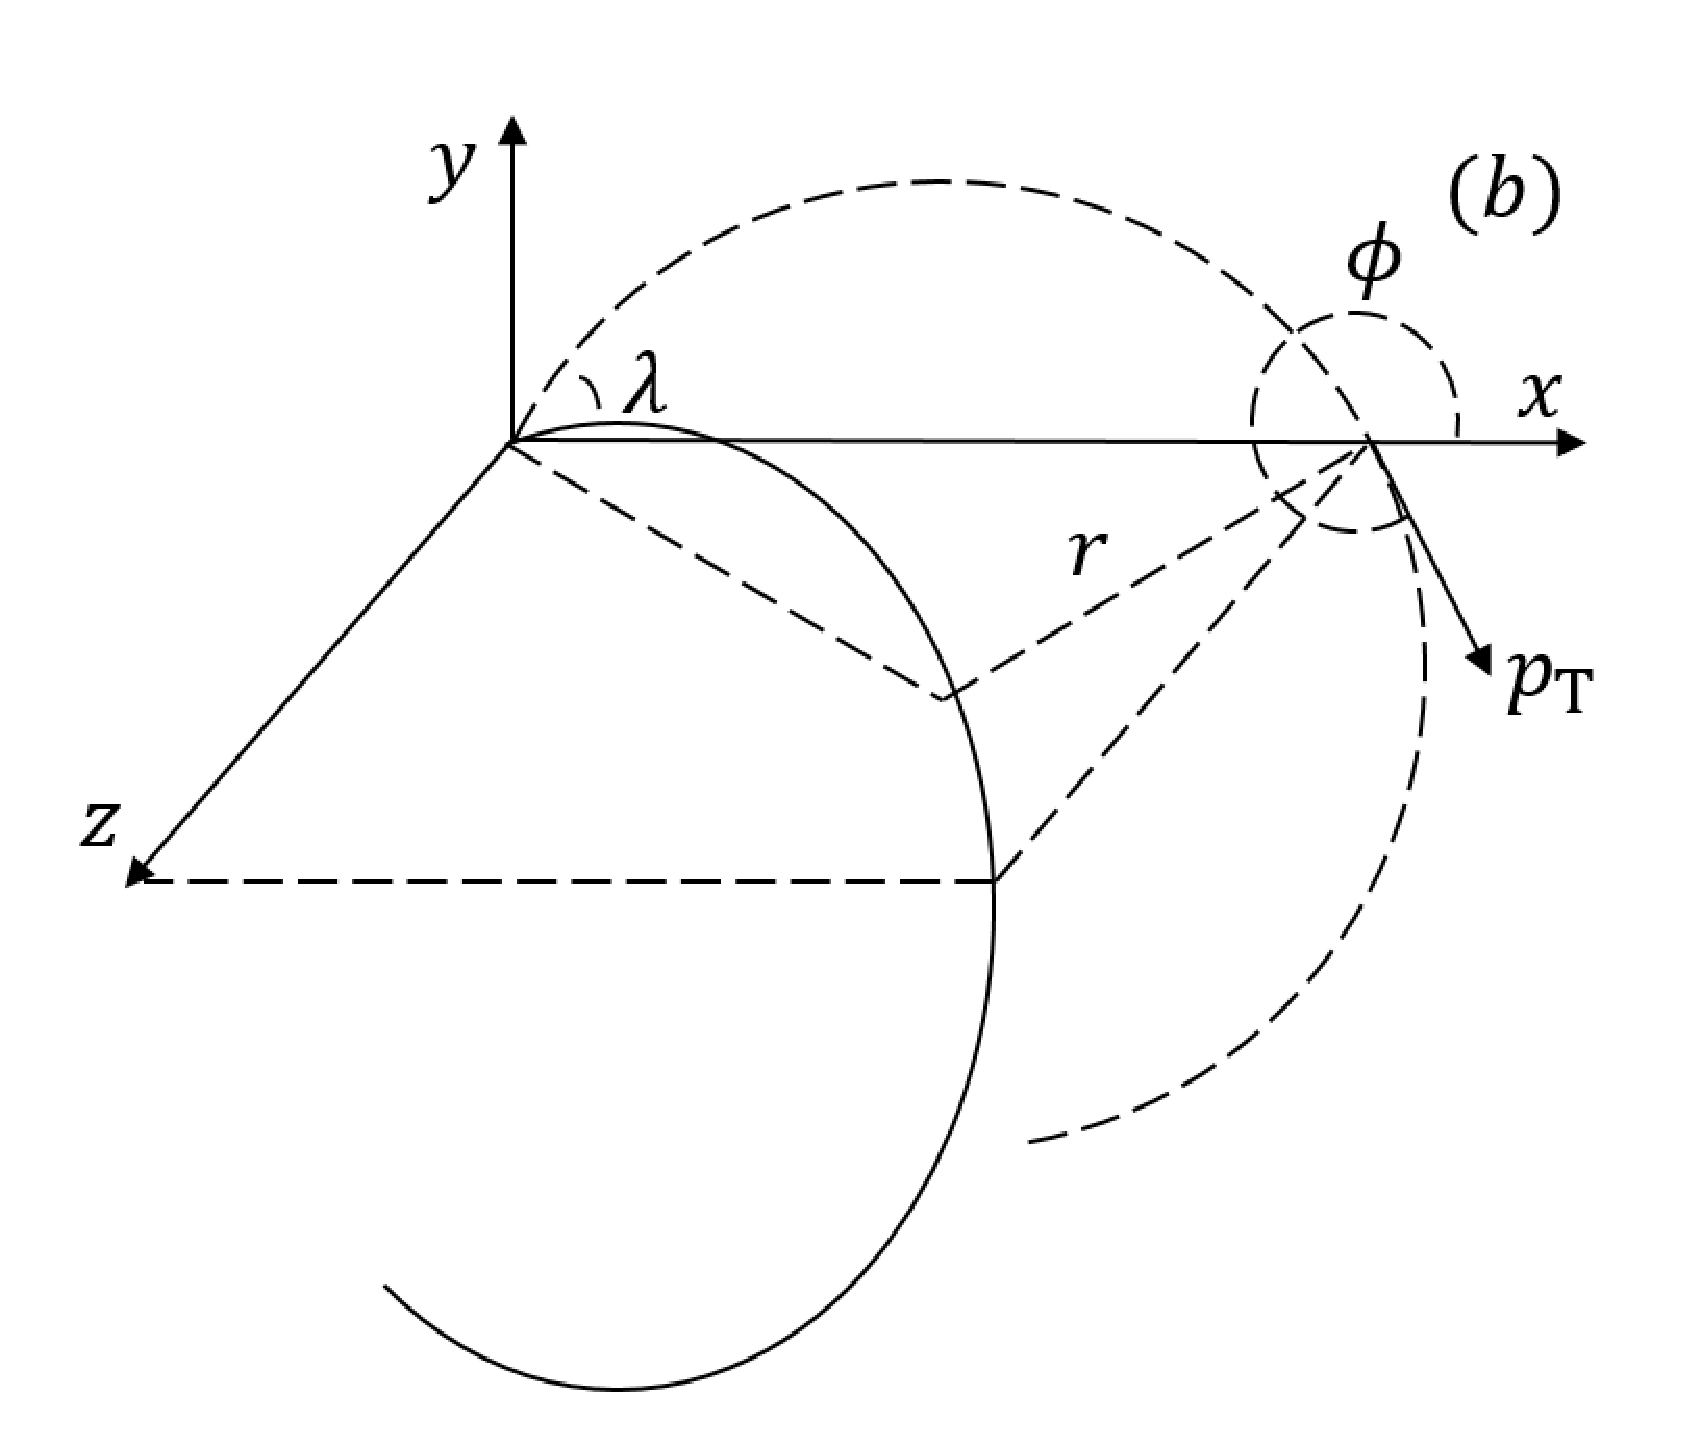
\includegraphics[width=\textwidth]{figures/ch5-KF_NDGAr/Variables_Diagram_new.eps}
     %     \caption{}
     %     \label{fig:Var}
     % \end{subfigure}
        \caption[Diagram of the simplified detector geometry.]{ Diagram of the simplified detector geometry, showing the direction of the magnetic field and the position of one of the radial pad layers. } \label{fig:DetectorFastSim}
\end{figure}

Each simulated particle is defined by specifying its type, charge, transverse momentum, $p_{\text{T}}$, azimuth angle, $\phi$, dip angle tangent, $\tan\lambda$, and the starting position. From this information, the initial MC-true (henceforth ``true'') state vector $s_0^{\text{true}}$ is built. The true state vector is moved through the detector by applying the same operations of the propagation steps of \texttt{CKF} in reverse, moving from layer to layer of pads.

The propagation of the state vector is obtained by applying Eq.~\ref{eq:func}. At each step the energy loss is calculated using the Bethe-Bloch formula as described in Eq.~\ref{eq:Bethe} and multiplying by the distance traveled and the material density. The energy loss is then converted in the $q/{p_{\text{T}}}$ multiplicative factor described in Eq.~\ref{eq:func} and smeared with a Landau distribution having a width equal to the $c_k$ factor described in Eq.~\ref{eq:eloss-factor}. The multiple scattering effects are simulated by calculating the scattering angle distribution root mean square $\theta_{\textrm{M}}$ and from that the process noise matrix $Q$. The diagonal elements of the matrix are then used as the widths of smearing Gaussian distributions that are applied to parameters $s_2=\sin\phi,s_3=\tan\lambda$ and $s_4=q/p_{\text{T}}$. To reproduce the measurement noise encapsulated in matrix $R$, a Gaussian smearing is applied to the position parameters $s_0=y$ and $s_1=z$. The widths of the distributions are equal to the position resolutions $\sigma_{r\phi}$ and $\sigma_{z}$ respectively. Note that the energy loss and multiple scattering elements of the simulation as well as the relative corrections applied in the reconstruction could be applied and set independently, similarly to what was done for the ND-GAr-Lite Toy Monte Carlo tool described in Sec. \ref{Sec:ToySim-Lite}.

The propagation continues until any of the following happens: the particle reaches the edges of the detector cylinder; the particle looses all its remaining energy; the track has traversed a predefined maximum number of points; one of the propagation steps fails.  Once the track is fully generated, the track fit is done as described in Sec.~\ref{Sec:KalGAr}. No element of track formation or particle identification is included. After saving all information, a new simulation and track fit start.

\section{\texttt{GArSoft} for ND-GAr}
\label{Sec:GArSoft-GAr}
As already described in Sec. \ref{Sec:GArSoft_Lite} \texttt{GArSoft} is the software toolkit which handles the simulation and reconstruction of events inside ND-GAr and ND-GAr-Lite \cite{garsoft}. The event generation and particle propagation are shared between the two detectors and are outlined in Sec. \ref{Sec:GArSoft_PartGen}. The TPC signal formation, digitization and reconstruction however are completely separate for ND-GAr and will be described in this section.

\subsection{TPC signal formation, digitization and hit finding}
\label{GArSoft_signal}
The \texttt{GArSoft} signal formation for ND-GAr's TPC takes the energy deposits produced by Geant4 as input (see Sec. \ref{Sec:GArSoft_PartGen}). These are used to simulate ionization in the gaseous medium using an un-tuned Birks' model for recombination \cite{Birks:1951boa}. The simulation of the scintillation photons that would be produced by the passing particle is not yet implemented. The ionized electrons drift is simulated by numerically integrating over the longitudinal and transverse diffusion distributions using a constant drift velocity and exponential electron lifetime factor. Electrons are registered on the nearest readout pads after the diffusion simulation has displaced them by a random
amount proportional to the square root of the drift time. Note that the readout-pads are placed radially at the two ends of the TPC cylinder, similarly to what was described for \texttt{fastMCKalman}. 

Since the exact electronics to be paired to the MWPC has not yet been decided, no pulse shaping by the read-out electronics nor any noise is yet simulated in \texttt{GArSoft} and the signal gain is arbitrarily set. The Analog to Digital Converter (ADC) sampling period is assumed to be 198 ns with an event readout containing 18048 samples. Raw wave-forms are saved as \enquote{raw digits} with no suppression using a simple thresholding technique.

In \texttt{GArSoft} a hit refers to a pulse that has been found and fit on a single channel, following the convention defined by LArSoft. A hit-finding algorithm is used in \texttt{GArSoft} to identify the over-threshold blocks in the raw digits that can be mapped onto hits. In the case they surpass a threshold length or the waveform is found to dip below a fraction of their maximum and go back up again, the hits are split. Finally, in order to reduce their number and improve their spacial resolution, nearby hits in time and space are grouped in hit clusters. The charge centroids of the hit clusters are then found and saved. 

\subsection{Track formation}
\label{GArSoft_TrackForming}
Track identification in \texttt{GArSoft} proceeds in two steps: first the hit clusters are collected into segments called vector hits, then these are combined together into track candidates. Vector hits are identified using linear fits on the hit clusters as a function of $(x,y,z)$. An initial segment of 10 cm is defined by choosing a pair of hit clusters and finding the line passing through them. All hit clusters that lie at most 2cm away from the segment are added to the vector hit. Every time a cluster is added the line segment is refit. Six linear 2D fits are applied, choosing all combinations of coordinate pairs and directions. To define the 3D direction of the vector hit the independent coordinate of the fit is chosen to be the one with the smallest sum of absolute values of slopes. Once all clusters are assigned to vectors, a check on the quality of the fits is performed: if the values of the $\chi^2$'s surpass a threshold value the clusters contained in a vector are released and they are either added to other vector hits or used to form new ones.

Once the vector hits are found they are grouped to form track candidates following a series of criteria. Specifically a vector hit is added to a track candidate if it passes the criteria for at least one of the vector hits already in the track candidates. To describe the test conditions we'll use the following notation: the position and direction vectors of the test vector hit already in the track are written as $\Vec{p}_i$ and $\Vec{v}_i$ respectively, while the same quantities for the vector hit candidate are written as $\Vec{p}_c$ and $\Vec{v}_c$.

The first condition is that the dot product between the directions doesn't surpass a threshold of 0.9:
\begin{equation}
    |\Vec{v}_c\cdot\Vec{v}_i|<0.9.
\end{equation}
A condition is also imposed on the distance between the vector hits, which must be at most 60cm:
\begin{equation}
    |\Vec{p}_c-\Vec{p}_i|<60 \text{cm}.
\end{equation}
Vector hits must also points towards each other. This can be checked using the \enquote{miss distance} which is defined as the cross product between the vector distance between the two centers of the vector hits and their directions. The condition is that the miss-distances must be smaller that 6 cm:
\begin{equation}
    \begin{aligned}
    |(\Vec{p}_c-\Vec{p}_i)\times\Vec{v}_i|&<6cm, \\
    |(\Vec{p}_c-\Vec{p}_i)\times\Vec{v}_c|&<6cm. 
    \end{aligned}   
\end{equation} 
To form a track candidate the vector hits also need to lie on a circle in the $xy$ plane, which is parallel to the direction of the electric and magnetic fields in the TPC. For this to be true the average of the directions must point along
the displacement between the centers. We define the $xy$ plane displacement between the vector hit centers as:
\begin{equation}
    \Vec{t}=\hat{x}(\Vec{p}_i-\Vec{p}_c)\cdot\hat{x}+\hat{y}(\Vec{p}_i-\Vec{p}_c)\cdot\hat{y},
\end{equation}
where $\hat{x},\hat{y},\hat{z}$ are the unit vectors along the $x$, $y$ and $z$ directions respectively. We define the 2D unit vectors pointing along the vector hits in the $xy$ plane as:
\begin{equation}
    \begin{aligned}
    \Vec{u}_i&=\frac{\hat{x}\Vec{v}_i\cdot\hat{x}+\hat{y}\Vec{v}_i\cdot\hat{y}}{|\hat{x}\Vec{v}_i\cdot\hat{x}+\hat{y}\Vec{v}_i\cdot\hat{y}|}, \\ \\
    \Vec{u}_c&=\frac{\hat{x}\Vec{v}_c\cdot\hat{x}+\hat{y}\Vec{v}_c\cdot\hat{y}}{|\hat{x}\Vec{v}_c\cdot\hat{x}+\hat{y}\Vec{v}_c\cdot\hat{y}|}.  
    \end{aligned}   
\end{equation} 
We can now define the signed direction sum as:
\begin{equation}
    \Vec{s}=\Vec{u}_i+\frac{\Vec{u}_c\cdot\Vec{u}_i}{|\Vec{u}_c\cdot\Vec{u}_i|}\Vec{u}_c.
\end{equation}
Finally we can define $\eta$ as :
\begin{equation}
    \eta = \left|\frac{\Vec{s}}{|\Vec{s}|\times\Vec{t}}\right|,
\end{equation}
which is used for the condition $\eta<1.2$ cm. Unlike the previous criteria which are only applied to individual couples of vectors, the $\eta$ test is applied between the candidate and test vector as well as all the other vectors belonging to the track candidate within a 20 cm radius; if just one of the tests fails the match is dropped.

The final test is a required match between the vector hits, where $\lambda$ is computed as:
\begin{equation}
    \begin{aligned}
        \lambda_i&=\tan^{-1}\left(\frac{|\hat{z}\cdot\Vec{v}_i|}{\sqrt{(\hat{y}*\Vec{v}_i)^2+(\hat{x}\cdot\Vec{v}_i)^2}}\right),\\\\
        \lambda_c&=\tan^{-1}\left(\frac{|\hat{z}\cdot\Vec{v}_c|}{\sqrt{(\hat{y}*\Vec{v}_c)^2+(\hat{x}\cdot\Vec{v}_c)^2}}\right),
    \end{aligned}
\end{equation}
for the test and candidate vector respectively. The match condition is :
\begin{equation}
    |\lambda_i-\lambda_c|<0.05.
\end{equation}
An additional requirement on the relative signs of the slopes is applied only if the absolute value of the $z$ component of $\Vec{v}_i$ and $\Vec{v}_c$ both exceed 0.01:
\begin{equation}
    (\Vec{v}_c\cdot\Vec{v}_i)(\Vec{v}_c\cdot\hat{z})(\Vec{v}_i\cdot\hat{z})>0.
\end{equation}
Once all the hit clusters are assigned to track candidates their order within the track is defined using a sorting algorithm. The first step in the sorting procedure consists in finding all the distances between the hit clusters. Then two links per for each point are defined purely based on shortest-distance arguments, avoiding the creation of cyclical loops. Finally a chain is created matching the links. Tracks and hit clusters are assigned to MC-truth particles using a back-tracker.

While the current track finding implementation in \texttt{GArSoft} is in a relatively mature state, some issues exist that need to be acknowledged. The algorithm has a tendency of adding vector hits to the wrong track or joining two tracks together. This happens most often close to neutrino interaction vertexes where many particles tracks are formed close in position and direction. The error is also relatively common in the case of the electron and positron tracks produced in photon conversions. The opposite error, consisting in breaking longer tracks in smaller segments, is also relatively common. This can happen for a variety of reasons: track may have a scatter \enquote{kink} partway along it, or a delta ray may be emitted, or some hit clusters from another track may get mis-assigned to a vector hit, causing it to point in the wrong direction or to be displaced from the track. This effect is again especially noticeable close to the primary interaction vertex, where hit clusters from more than one track can be confused and vector hits may point in the wrong direction. Ways to improve the performance of the pattern recognition could include allowing the track fitter to reassign TPC clusters to tracks, or to make a second pass through hit assignment once the track parameters have been estimated.
\subsection{Track Fitting}
\label{Sec:GArSoft_Fit}
To compute the best estimates of the track parameters on both ends of the track, \texttt{GArSoft} employs an algorithm based on the Kalman Filter technique. While several aspects of this fitter are different from what was described in Sec. \ref{Sec:KalGAr}, the key operational steps are identical. From now on we will refer to the original \texttt{GArSoft} Kalman Filter algorithm as the \texttt{GKF}.

We start by defining the state vector parametrization used to identify the track helix trajectories in the TPC. As discussed in Sec. \ref{Sec:KalGAr} to uniquely define any helix trajectory produced by a charged particle in a magnetic field, one needs a 5-dimensional state vector which is a function of a sixth free parameter. Keeping the same coordinate system originally defined in Sec. \ref{Sec:KFLite} and \ref{Sec:KalGAr} the \texttt{GArSoft} parametrization uses $z$ as the free parameter and defines the state vector as:
\begin{equation}
    s_G = (y,x,1/r,\phi,\lambda)
\end{equation}
where all the parameters are defined identically to the parameters in \ref{eq:state}. The main difference with the ALICE parametrization used for the \texttt{BKF} and \texttt{CKF} consists in the choice of $z$ as the free parameter and the use of $\phi$ instead of $\sin{\phi}$. The use of $z$ as the free parameter is somewhat problematic. This is because for the tracks produced in ND-GAr, which are expected to be mostly forward going, the motion in the direction of the magnetic field is typically small. Additionally, by choosing the free parameter $x$ (as for the \texttt{CKF} or \texttt{KF-Lite}) the algorithm steps are naturally defined by the different pad layers. The identification is less straight-forward if $z$ is chosen. The state vector is evolved along the helix trajectory using the propagator function:

\begin{equation} \label{eq:funcGAr}
    \widetilde{s}_G^k = f_{k-1}(s_G^{k-1}) =
        \left\{
        	\begin{aligned}
        		& \widetilde{y}_k  =  y_{k-1}+  \Delta z_k\cot{\lambda_{k-1}}\sin{\phi_{k-1}},  \\
        		& \widetilde{x}_k  =  x_{k-1}+\Delta z_k\cot{\lambda_{k-1}}\cos{\phi_{k-1}} ,\\ 
                    & 1/\widetilde{r}_k =  1/r_{k-1},  \\               
                    & \widetilde{\phi}_k   =  \phi_{k-1}+\Delta z_k(1/r_{k-1})\cot\lambda_{k-1}, \\   
                    & \widetilde{\lambda}_k = \lambda_{k-1},
        	\end{aligned}
        \right.
\end{equation}

where $\Delta z_k$ is the distance in the $z$ direction between the previous and current point. The propagation matrix, $F_k$, is calculated as the Taylor expansion coefficient $\partial f_k/ \partial s_k$, as described in Eqs. \ref{eq:jacobian} and \ref{eq:jacobian2}.

It's important to note that the evolution equation for the $\phi$ angle makes use of a small angle approximation $\Delta sin\phi_k\simeq \Delta \phi_k$. Analogously the evolution equations for the $y$ and $x$ parameter approximate an arch motion with a segment linear motion. This is not true for the evolution function described in Eq. \ref{eq:func} where all formulas were exact. While this approximation is well justified in the case the consecutive points in the track are very close together, it can produce errors if the condition is not met. This limitations make it so that the \texttt{GKF} isn't problematic for tracks confined inside the TPC, but it is in case of large gaps making the connection points from other detector elements (i.e. ND-LAr or the ECAL) complex. By using the angle $\phi$ rather than its sine, however, the algorithm partially avoids the semi-circle limitation discussed in Sec. \ref{Sec:KalGAr} and is allowed to propagate for an entire circle. 

Another key difference with the \texttt{CKF} algorithm is that no energy loss treatment is implemented. The $1/r$ parameter is left completely static and no factor such as the one described in Eq. \ref{eq:eloss-factor} is added to $F_k$. As it will be shown in Sec. \ref{Sec:Garsoft_Implementation} this omission produces biases in the momentum estimation, especially in the case of heavier particles such as protons. Similarly, no treatment of multiple scattering is implemented in the algorithm. A process noise matrix $Q$ is added to the covariance matrix as described in Eq. \ref{eq:pcov}, but rather than being derived using the Molière angle as described in Eq. \ref{eq:Q}, it is set as a constant arbitrary term:

\begin{equation}\label{eq:Q2}
    Q =\begin{bmatrix}
    0 & 0 & 0 & 0& 0 \\
    0 & 0 & 0 & 0& 0 \\
    0 & 0 & 10^{-9} & 0& 0 \\
    0 & 0 & 0 & 10^{-9}& 0 \\
    0 & 0 & 0 & 0& 10^{-4} \\
    \end{bmatrix} .
\end{equation}
Not evaluating the effects of multiple scattering punctually, is bound to produce an incorrect estimation of the uncertainties related to angle and momentum terms, damaging the precision that the algorithm is able to achieve. The noise matrix $R$ is also left static using the resolution factors $\sigma_y=\sigma_x=2 \text{cm}$, which are chosen arbitrarily and don't reflect the actual resolutions of the hit clusters. The filtering step of the algorithm is performed in the standard way as described in Eq. \ref{eq:updates}.

The seeding procedure which was paired to the \texttt{GKF} consists in the \texttt{ILRM} algorithm described in Sec. \ref{Sec:SeedingLite}. The \texttt{ILRM} algorithm only provides an initial estimate for the state vector $s_0^G$. The initial covariance matrix $C_0$ is not estimated and is set arbitrarily as:

\begin{equation}
    \label{eq:C0}
    C_0 =\begin{bmatrix}
    1 & 0 & 0 & 0& 0 \\
    0 & 1 & 0 & 0& 0 \\
    0 & 0 & 0.25 & 0& 0 \\
    0 & 0 & 0 & 0.25& 0 \\
    0 & 0 & 0 & 0& 0.25 \\
    \end{bmatrix} .
\end{equation}

While only a very rough estimate of the initial covariance matrix is needed for a Kalman Filter algorithm to function, if the uncertainties are assigned in a fully arbitrary way ,several steps of the algorithm are wasted determining the general shape of the matrix, reducing the final resolution. 

\subsection{Vertex finding and fitting}
\label{Sec: Vertexing}
The vertex-finding algorithm implemented in \texttt{GArSoft} takes as input all the track candidates identified for an event and groups them together based on the position of their endpoints.  A track endpoint is a candidate for vertexing with another track endpoint if they are within 12 cm of each other. Vertices are fit with a linear extrapolation from the endpoints of each track. A list of found vertices and tracks is kept so that a track is not vertexed with itself even if it loops around in the magnetic field, and two tracks cannot be vertexed with each other more than once. Tracks and track ends may contribute to more than one candidate vertex.
The vertex fitting algorithm used in \texttt{GArSoft} is not fully mature and several improvements are being considered. Using helical extrapolations of tracks from the ends, calculating the covariance matrix of the vertex spatial coordinates, and improving the track association selection criteria are all
things that can improve the vertexing.


\section{The toy Monte Carlo study}
\label{Sec:ToyMCStudy_GAr}

Similarly to what was described in Sec. \ref{Sec:ToyMCTests-Lite} \texttt{fastMCKalman} was firstly used to develop a series of tests that were meant to validate each aspect of the simulation separately. These consisted in modifying the simulation conditions, including the particle types, the resolution of the pads, and especially the energy loss and multiple scattering and investigating the performance of the \texttt{CKF} and \texttt{BKF} algorithms. This series of tests are described summarized in App. \ref{App:Summary_Tables}. 

Once all the aspects of the simulation and reconstruction were considered to be in a mature state, one final summary study was produced and described in a publication, which at the time of writing is under review for Computer Physics Communications \cite{Battisti:2024nqq}. The study focused on two specific samples, the first of which included a spectrum of different detector characteristics and particle properties and was used to validate the algorithm across a wide range of parameter space. To analyze this sample, a recently developed interactive data visualization tool called \texttt{ROOTInteractive} was used~\cite{RootInt}. The second sample was designed to produce performance estimates for a HPgTPC similar to ND-GAr. In this section we will focus on the results of this study, taking most of the material from the publication itself.
\subsection{Sample Definition}
\label{sec:Sample_Definition}
The aforementioned \texttt{fastMCKalman} was used to produce two separate samples, simulated in the same simplified gas TPC geometry. The TPC has a cylindrical form with a radius $r=250 \ \text{cm}$ and the length of the cylinder is taken as $L=500 \ \text{cm}$. There are 250 circular layers of pads placed radially at each of the two end caps ($z=\pm250~\textrm{cm}$). A magnetic field of intensity $B=0.5 \ T$ is placed in the drift direction along the cylinder axis. 

The first sample, which includes a total of $5\times10^5$ tracks, contains a wide variety of detector properties, particle types and energies and was used to validate the \texttt{CKF} algorithm and its \texttt{Seed} in as wide a parameter space as possible. We will refer to this sample as the parameter scan sample or PS sample. The PS sample is composed of two equally large sub-samples with different starting position distributions: a sample of primaries---emulated as in a collider event geometry---starting from the center of the detector $(x,y,z)=(0,0,0)\ \text{cm}$ and a sample of secondaries with randomized starting positions within a fiducial cylinder of radius $r=200 \ \text{cm}$ and length $l = 400 \ \text{cm}$. The initial spatial distribution of the secondaries in the sample is shown in Fig.~\ref{fig:ViewGAr}.

\begin{figure}[!ht]
     \centering
     \begin{subfigure}[b]{0.48\textwidth}
         \centering
         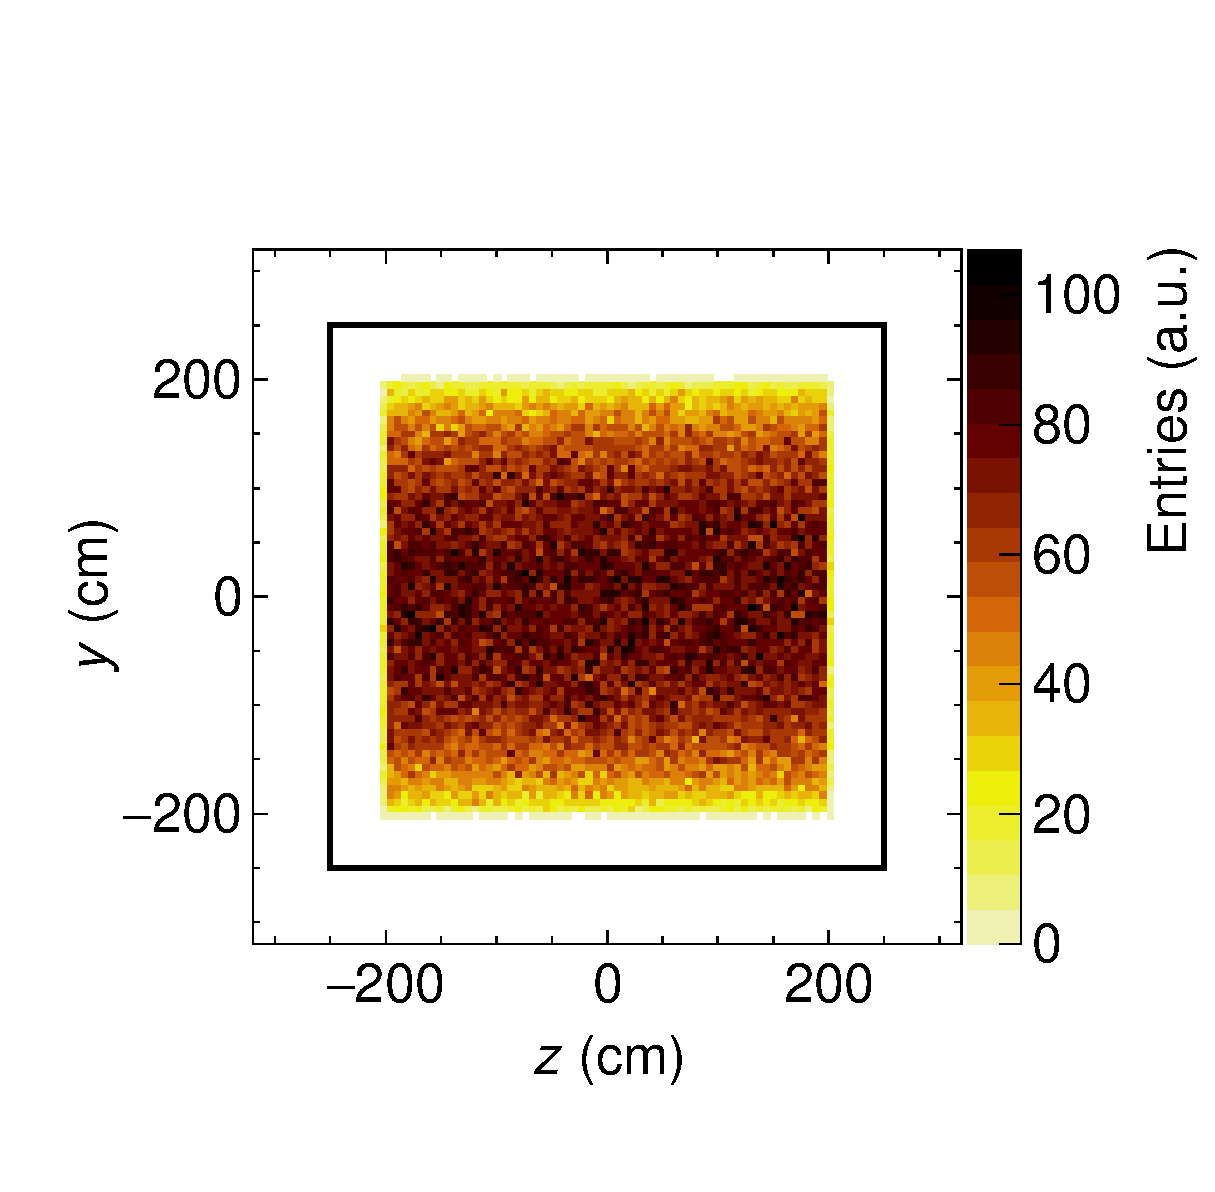
\includegraphics[width=\textwidth]{figures/ch5-KF_NDGAr/ToySample/testTPCMirrorYZ_view.eps}
         \caption{}
         \label{fig:YZViewGAr}
     \end{subfigure}
     \begin{subfigure}[b]{0.48\textwidth}
         \centering
         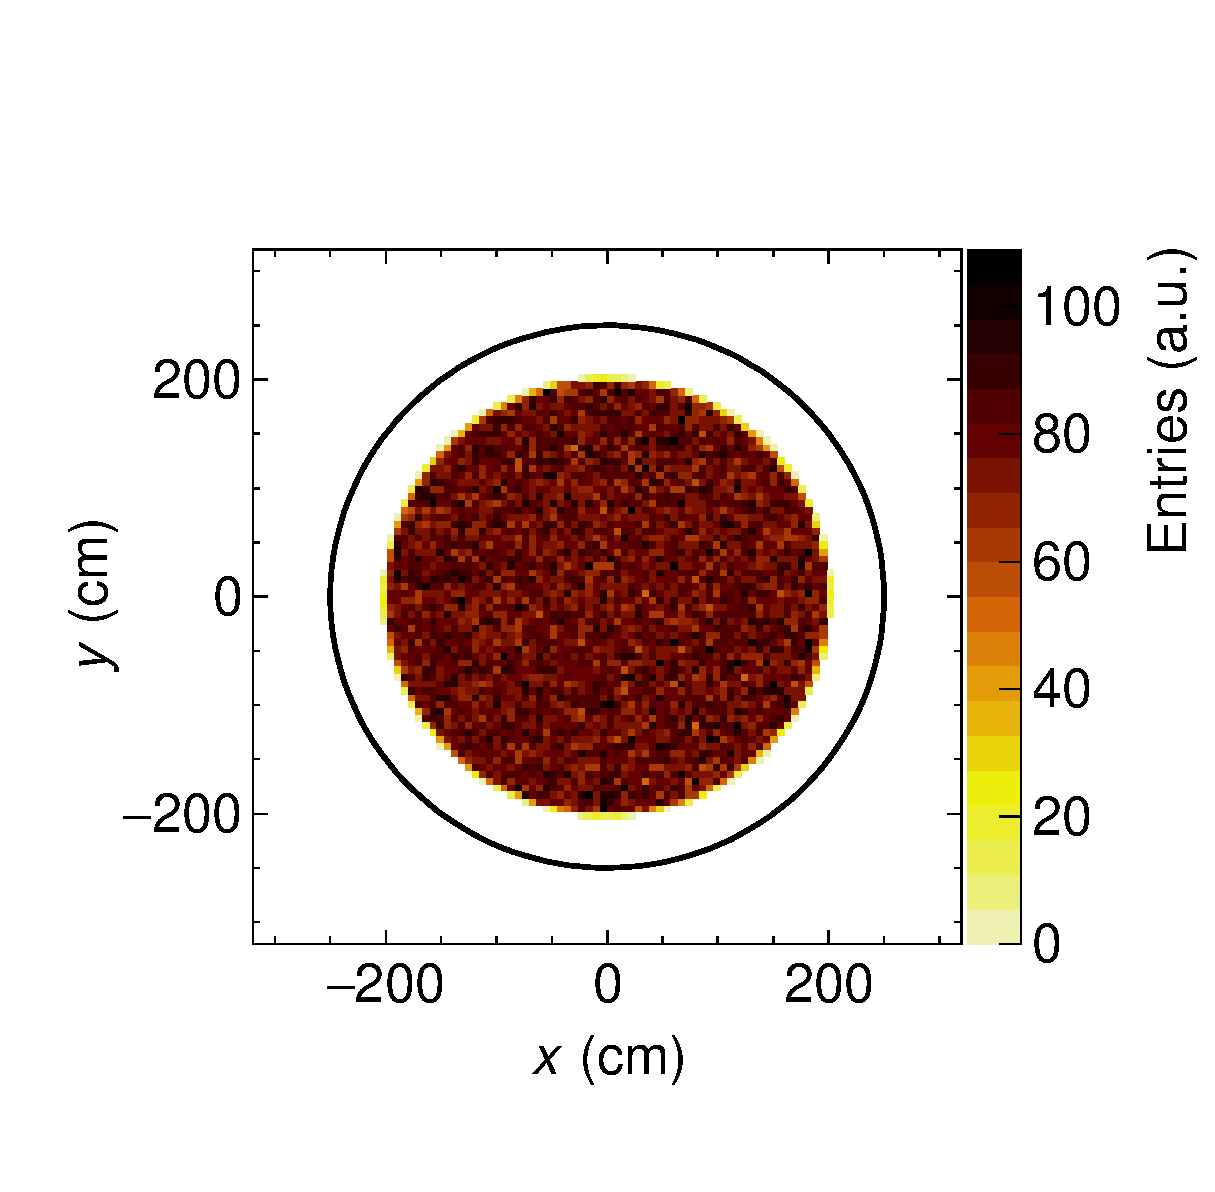
\includegraphics[width=\textwidth]{figures/ch5-KF_NDGAr/ToySample/testTPCMirrorXY_view.eps}
         \caption{}
         \label{fig:XYViewGAr}
     \end{subfigure}
        \caption[Starting positions for secondary particles in the PS sample.]{Starting positions for secondary particles in the PS sample. The primaries are not shown, as all of their starting positions are in $(x,y,z)=(0,0,0)$. The left plot shows the distribution in the $zy$ plane, while the plot on the right shows the distribution in the $xy$ plane. The edges of the TPC are drawn on top. } \label{fig:ViewGAr}
\end{figure}

The tracking pad response as well as the gas properties of the detector are sampled in each simulated event: the resolutions $\sigma_{r\phi}=\sigma_z$ are uniformly distributed between 0.1 cm and 0.5 cm and the pressure $P_\textrm{gas}$ was randomized between 0.1 atm and 10 atm. The gas composition was taken to be the Ne/CO2/N2 (90/10/5) gas mixture used by the ALICE experiment during Run-1~\cite{ALICE:2008ngc}. The radiation length and density of the gas at atmospheric pressure are $X_0=1.2763\times10^4 \ \text{cm}$ and $\rho = 0.0016265 \ \text{g/cm}^3$. The particles produced are equally divided in electrons, muons, pions, kaons and protons, corresponding to the ALICE’s convention for particle types, $t_{\textrm{ID}}$, 0, 1, 2, 3, and 4, respectively. The angles $\phi$ and $\lambda$ are fully randomized. The initial $p_{\textrm{T}}$ is sampled from a two-component distribution: a high-$p_{\text{T}}$ component uniformly distributed in $[0,20]$ GeV/c, which covers 70\% of the total, and a low-$p_{\text{T}}$ component flat in $1/p_\textrm{T}$:
\begin{equation} \label{eq:LowpT}
   p_{\textrm{T}}=\frac{p_{\textrm{T}_{\textrm{min}}}}{p_{\textrm{T}_{\textrm{min}}}/p_{\textrm{T}_{\textrm{max}}}+j},
\end{equation}
where $p_{\textrm{T}_{\textrm{min}}}=0.01$ GeV$/c$, $p_{\textrm{T}_{\textrm{max}}}=20 \ \text{GeV}/c$ and $j$ is a random variable uniformly distributed between 0 and 1. Some key properties of the tracks composing the PS sample are plotted in Fig.~\ref{fig:TPCProperties}. These include the $p_{\textrm{T}}$ spectrum, the lever arm $L_{\textrm{Arm}}$ and the number of points per track $N$ separated between primaries and secondaries. The lever arm is defined as the distance in the $xy$ plane between the first and last point in the track. All the tracks included in this and future plots have been successfully reconstructed, unless stated otherwise. %The PS sample track reconstruction efficiencies $\epsilon$ as a function of the same variables considered in Fig.~\ref{fig:TPCProperties} are shown in Fig.~\ref{fig:EffPS} in the Appendix. 

\begin{figure}[t]
     \centering
     \begin{subfigure}[b]{0.32\textwidth}
         \centering
         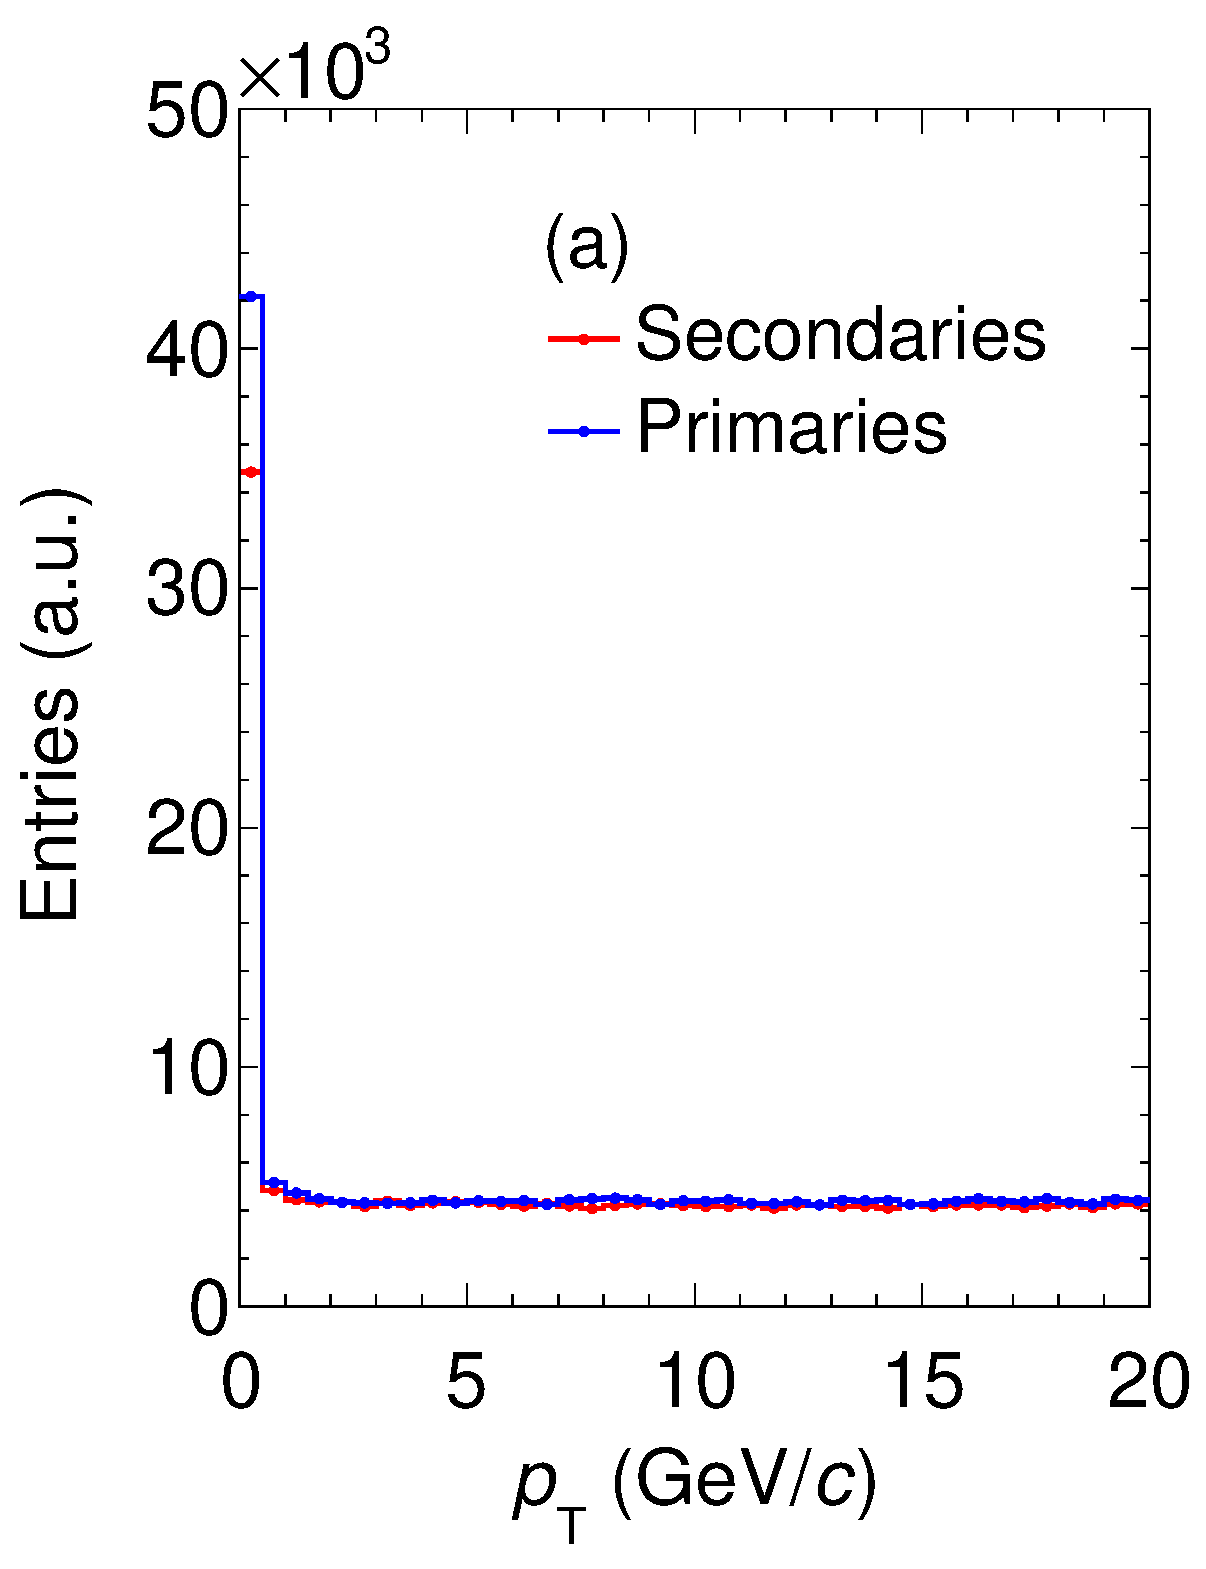
\includegraphics[width=\textwidth]{figures/ch5-KF_NDGAr/ToySample/testTPCMirrorpTAllTall.eps}
         \caption{}
         \label{fig:ptTPC}
     \end{subfigure}
     \begin{subfigure}[b]{0.32\textwidth}
         \centering
         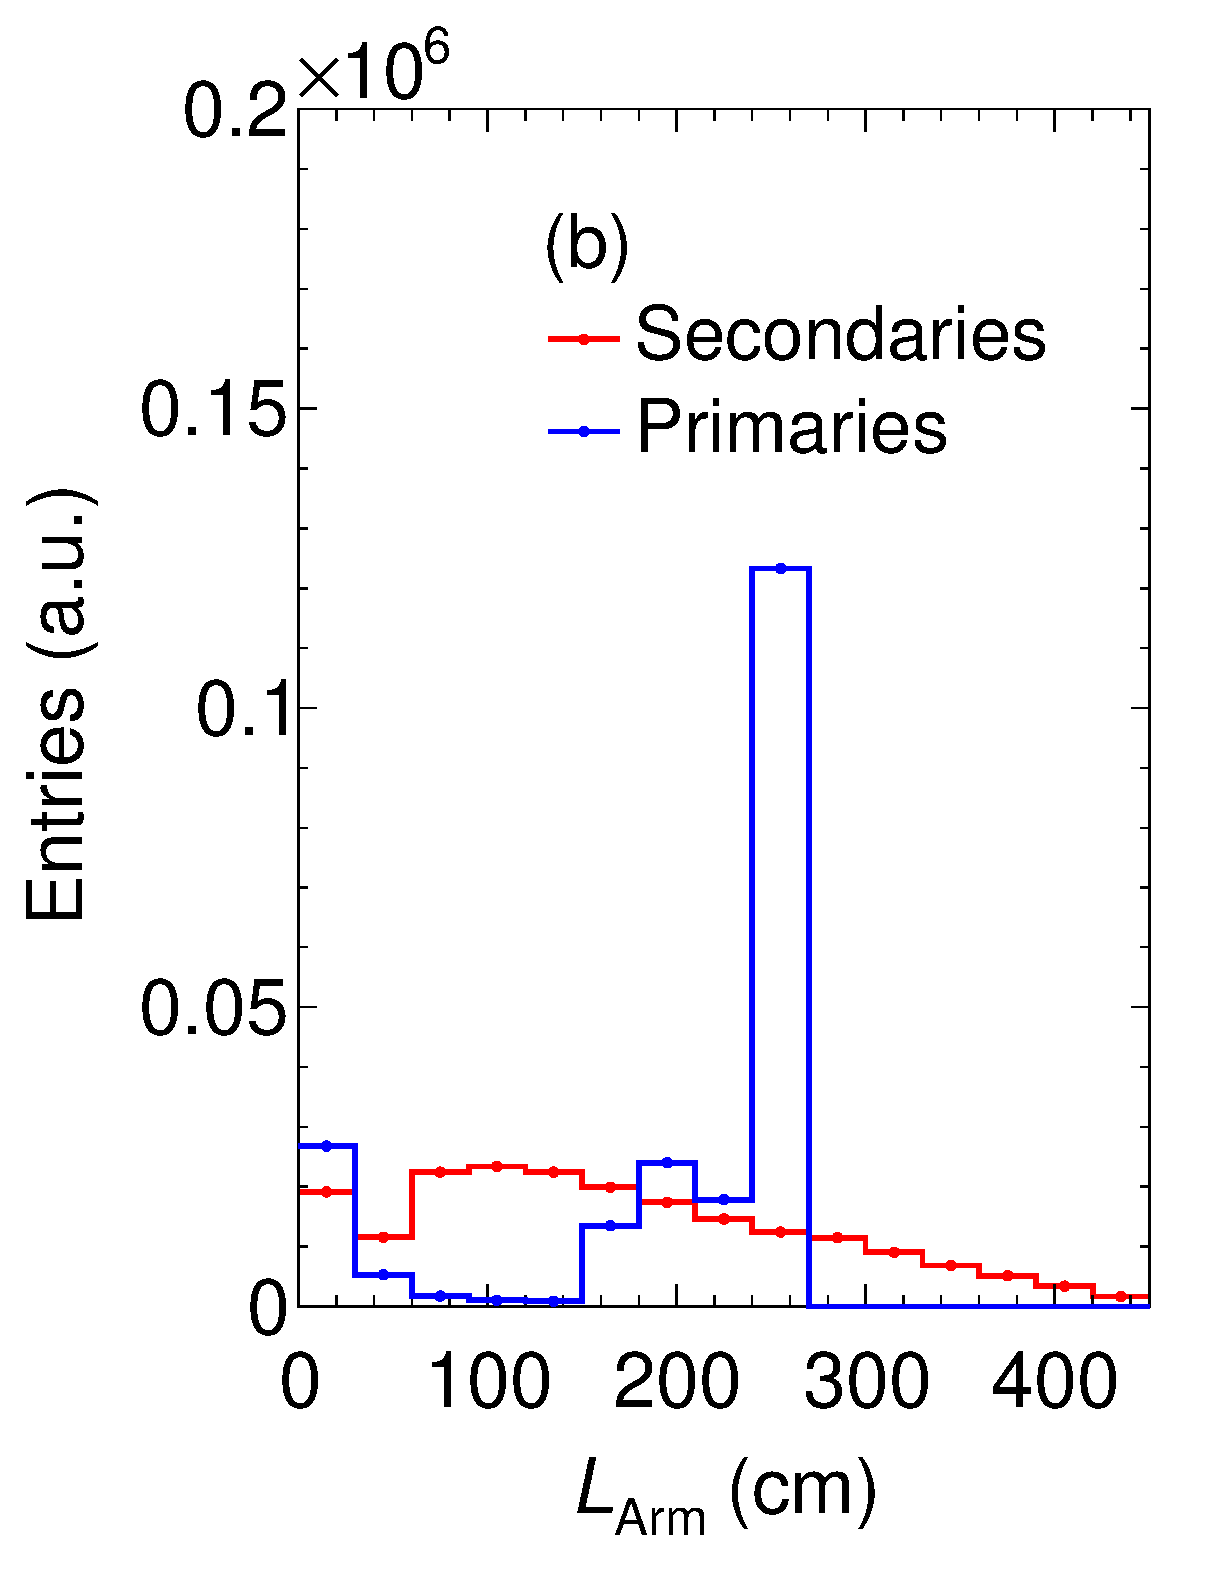
\includegraphics[width=\textwidth]{figures/ch5-KF_NDGAr/ToySample/testTPCMirrorLAllTall.eps}
         \caption{}
         \label{fig:LTPC}
     \end{subfigure}
          \begin{subfigure}[b]{0.32\textwidth}
         \centering
         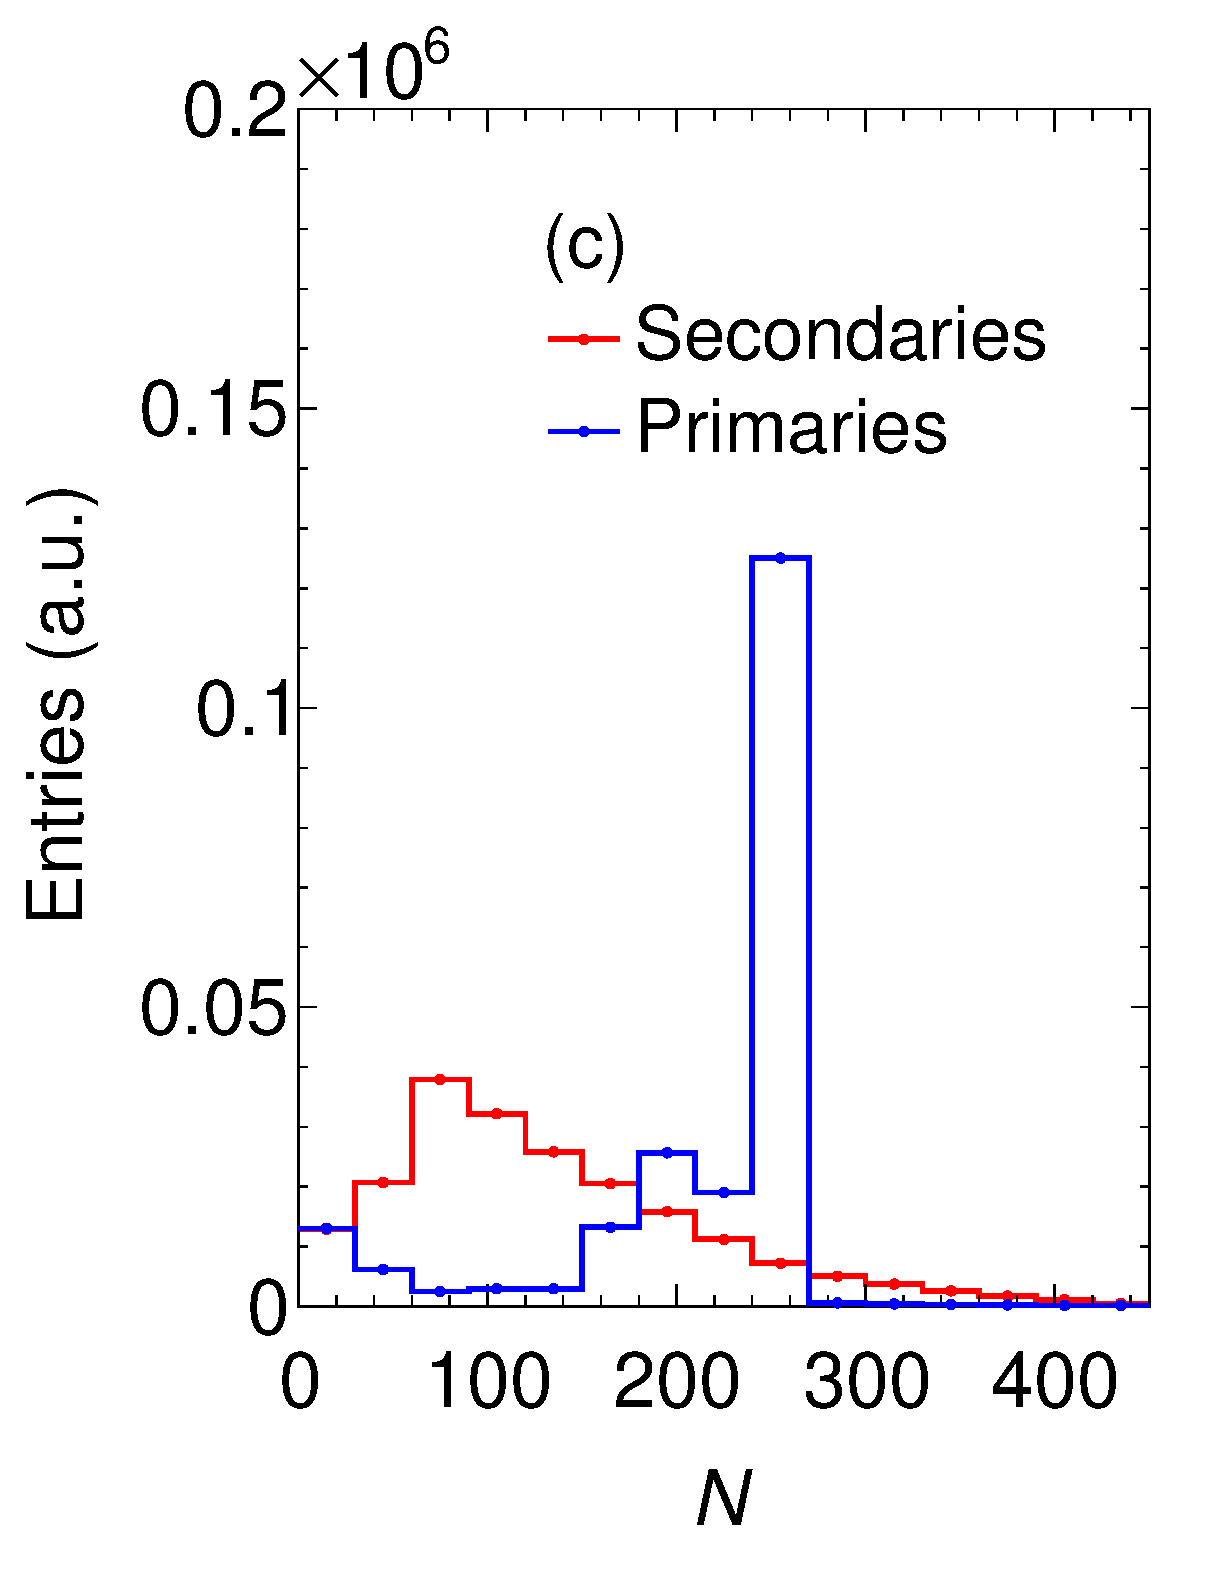
\includegraphics[width=\textwidth]{figures/ch5-KF_NDGAr/ToySample/testTPCMirrorNAllTall.eps}
         \caption{}
         \label{fig:NTPC}
     \end{subfigure}
        \caption[Distributions of (a) transverse momentum $p_{\textrm{T}}$,  (b) lever arm $L_{\textrm{Arm}}$ and (c) number of points per track $N$ in the PS sample.]{Distributions of (a) transverse momentum $p_{\textrm{T}}$,  (b) lever arm $L_{\textrm{Arm}}$ and (c) number of points per track $N$ in the PS sample. In all the plots the distributions for primary and secondary particles are shown separately. The low $p_{\textrm{T}}$ portion of the spectrum 
 is produced via Eq.~\ref{eq:LowpT}. The spikes around $N=250$ and $L_{\textrm{Arm}}=250$ in the primary sample are explained by the simulated geometry having 250 radial pad layers and the particles starting from the center of the detector. } \label{fig:TPCProperties}
\end{figure}

Primaries and secondaries have analogous $p_{\textrm{T}}$, but significant differences in their $L_{\textrm{Arm}}$ and $N$. Since the primaries all start at the center of the detector, most tracks will cross the detector exiting from the cylinder's barrel, producing a track with as many points as the 250 pad layers. In alternative the track can exit from the sides of the detector, producing tracks with a slightly smaller $N$ or be stopped inside the detector having $N<50$. For the secondaries the spread is much more homogeneous and the chance of producing tracks with $N>250$ is more significant.

A second sample containing a total of $10^5$ particle tracks was produced to recreate conditions analogous to the ones that would be experienced by a HPgTPC in a accelerator neutrino experiment, such as the ND-GAr detector. The goal for this second sample is to explore the potential performance of such a detector, using realistic particle spectra and spatial resolutions. This sample will be referred to as the high-pressure sample or HP sample. The HP sample is produced with randomized starting positions in the same manner as the ones applied to the secondaries in the PS sample. This is done to emulate the randomness of particle track formation in a neutrino experiment. The detector characteristics are fixed, having the same cylinder dimensions and pad distribution of the previous sample. The point resolutions are taken as $\sigma_{r\phi}=\sigma_z=0.1 \ \text{cm}$, comparable to what is quoted in ALICE~\cite{LIPPMANN2012}. The gas is a mixture of argon and methane at a 90 to 10 ratio at 10 atm of pressure, which is the nominal gas suggested for the ND-GAr detector in the DUNE Near Detector CDR~\cite{DUNE:2021NDCDR}. This composition corresponds to a $X_0=1.193 \times 10^3 \ \text{cm}$ and a density of $\rho = 0.01677 \ \text{g/cm}^3$. Only three particle types are considered in this case: muons, pions and protons. These were chosen because they are the key particles produced in $\nu_\mu$ charged-current interactions that are the most relevant in an accelerator neutrino experiment such as DUNE. The initial transverse momenta are randomized to be uniformly distributed between 0.01 GeV$/c$ and 5 GeV$/c$ and the angles are randomized  over the whole spectrum. The $p_{\text{T}}$, $L_\textrm{Arm}$ and $N$ distributions for the sample are shown in Fig.~\ref{fig:GArProperties}. %Similar to the PS sample, the reconstruction efficiencies are shown in the Appendix in Fig.~\ref{fig:EffHP}.

\begin{figure}[!ht]
     \centering
     \begin{subfigure}[b]{0.32\textwidth}
         \centering
         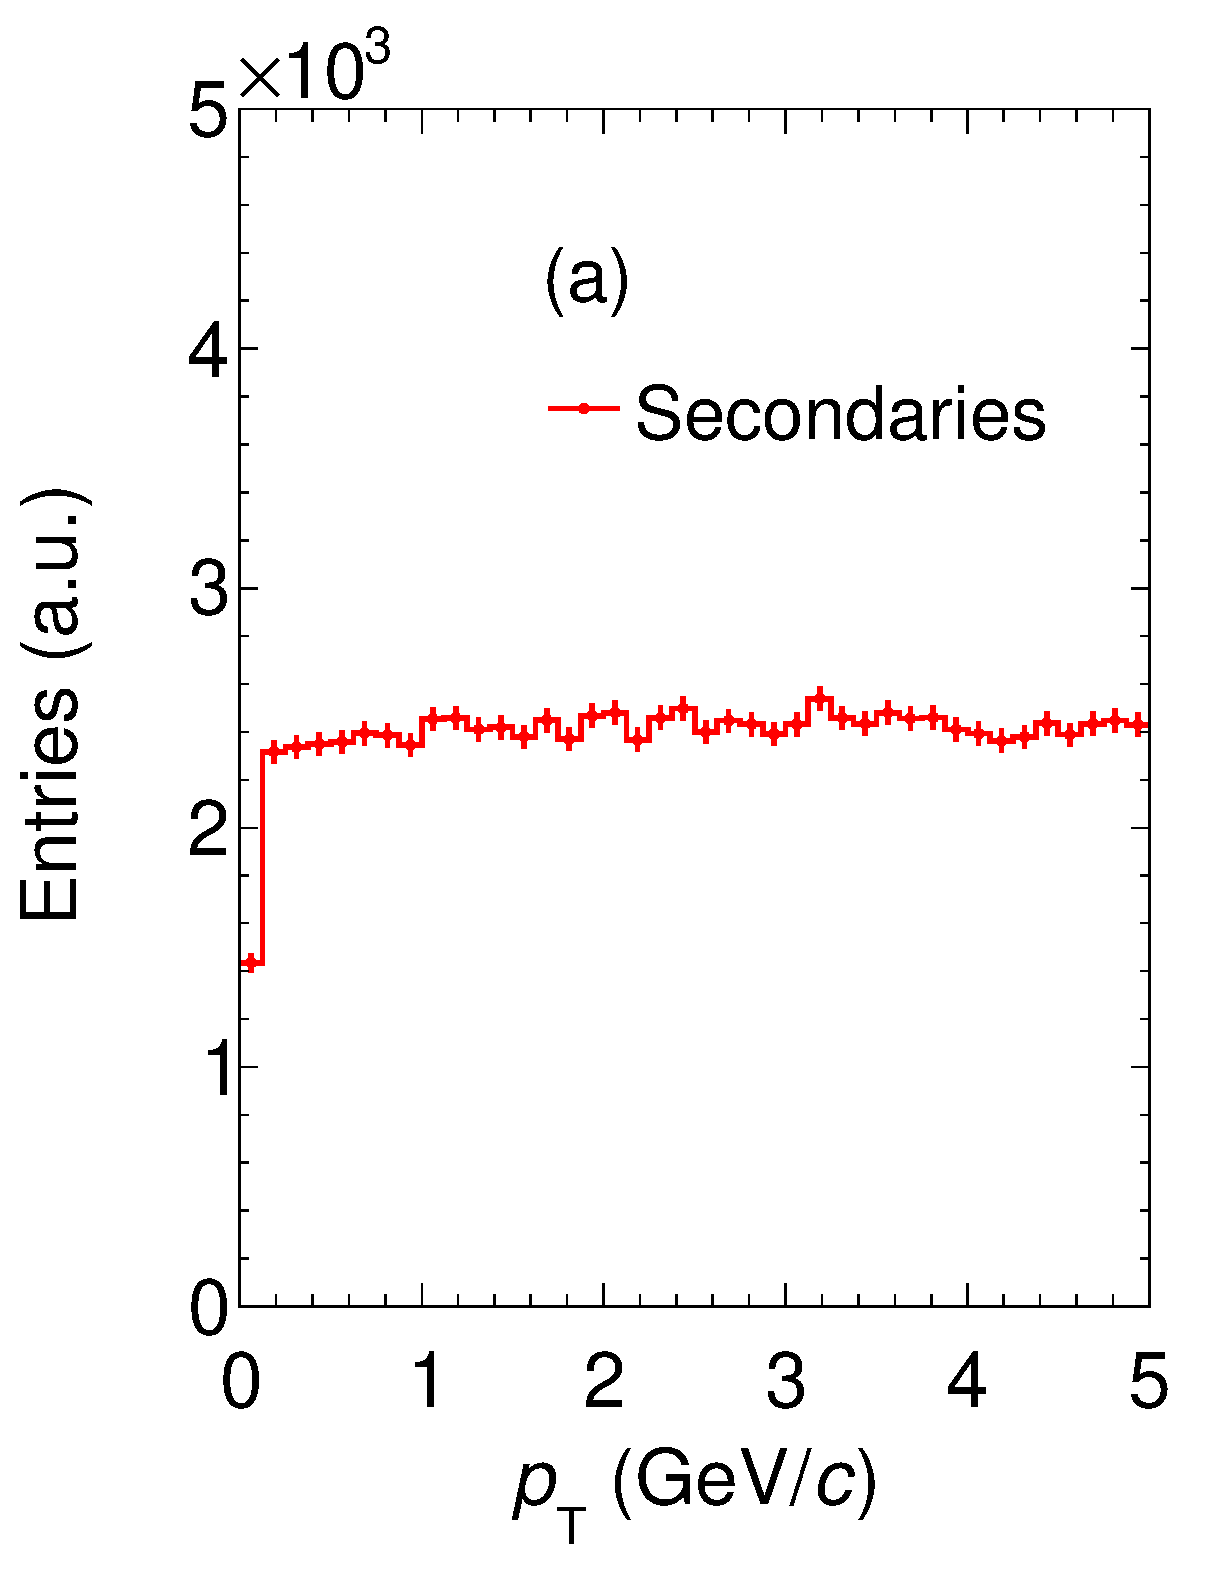
\includegraphics[width=\textwidth]{figures/ch5-KF_NDGAr/ToySample/testNDGArMirrorpTAllTall.eps}
         \caption{}
         \label{fig:ptGAr}
     \end{subfigure}
     \begin{subfigure}[b]{0.32\textwidth}
         \centering
         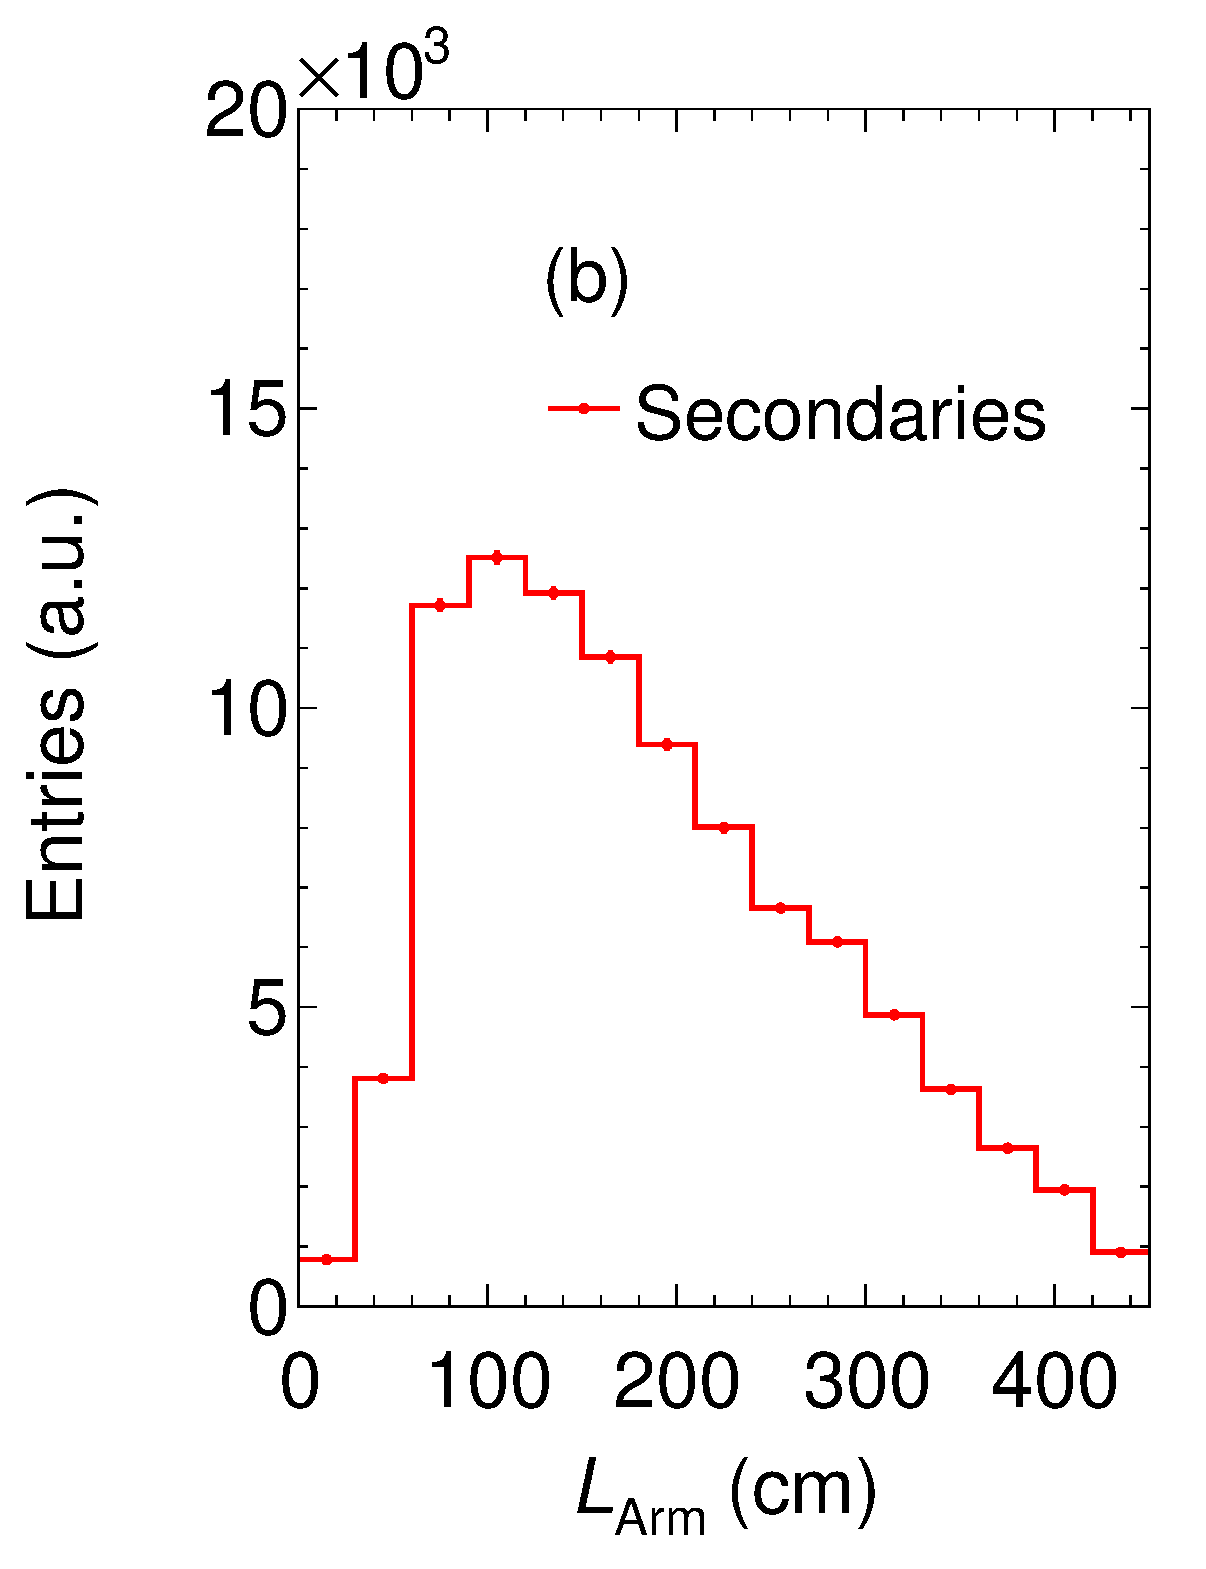
\includegraphics[width=\textwidth]{figures/ch5-KF_NDGAr/ToySample/testNDGArMirrorLAllTall.eps}
         \caption{}
         \label{fig:LGAr}
     \end{subfigure}
          \begin{subfigure}[b]{0.32\textwidth}
         \centering
         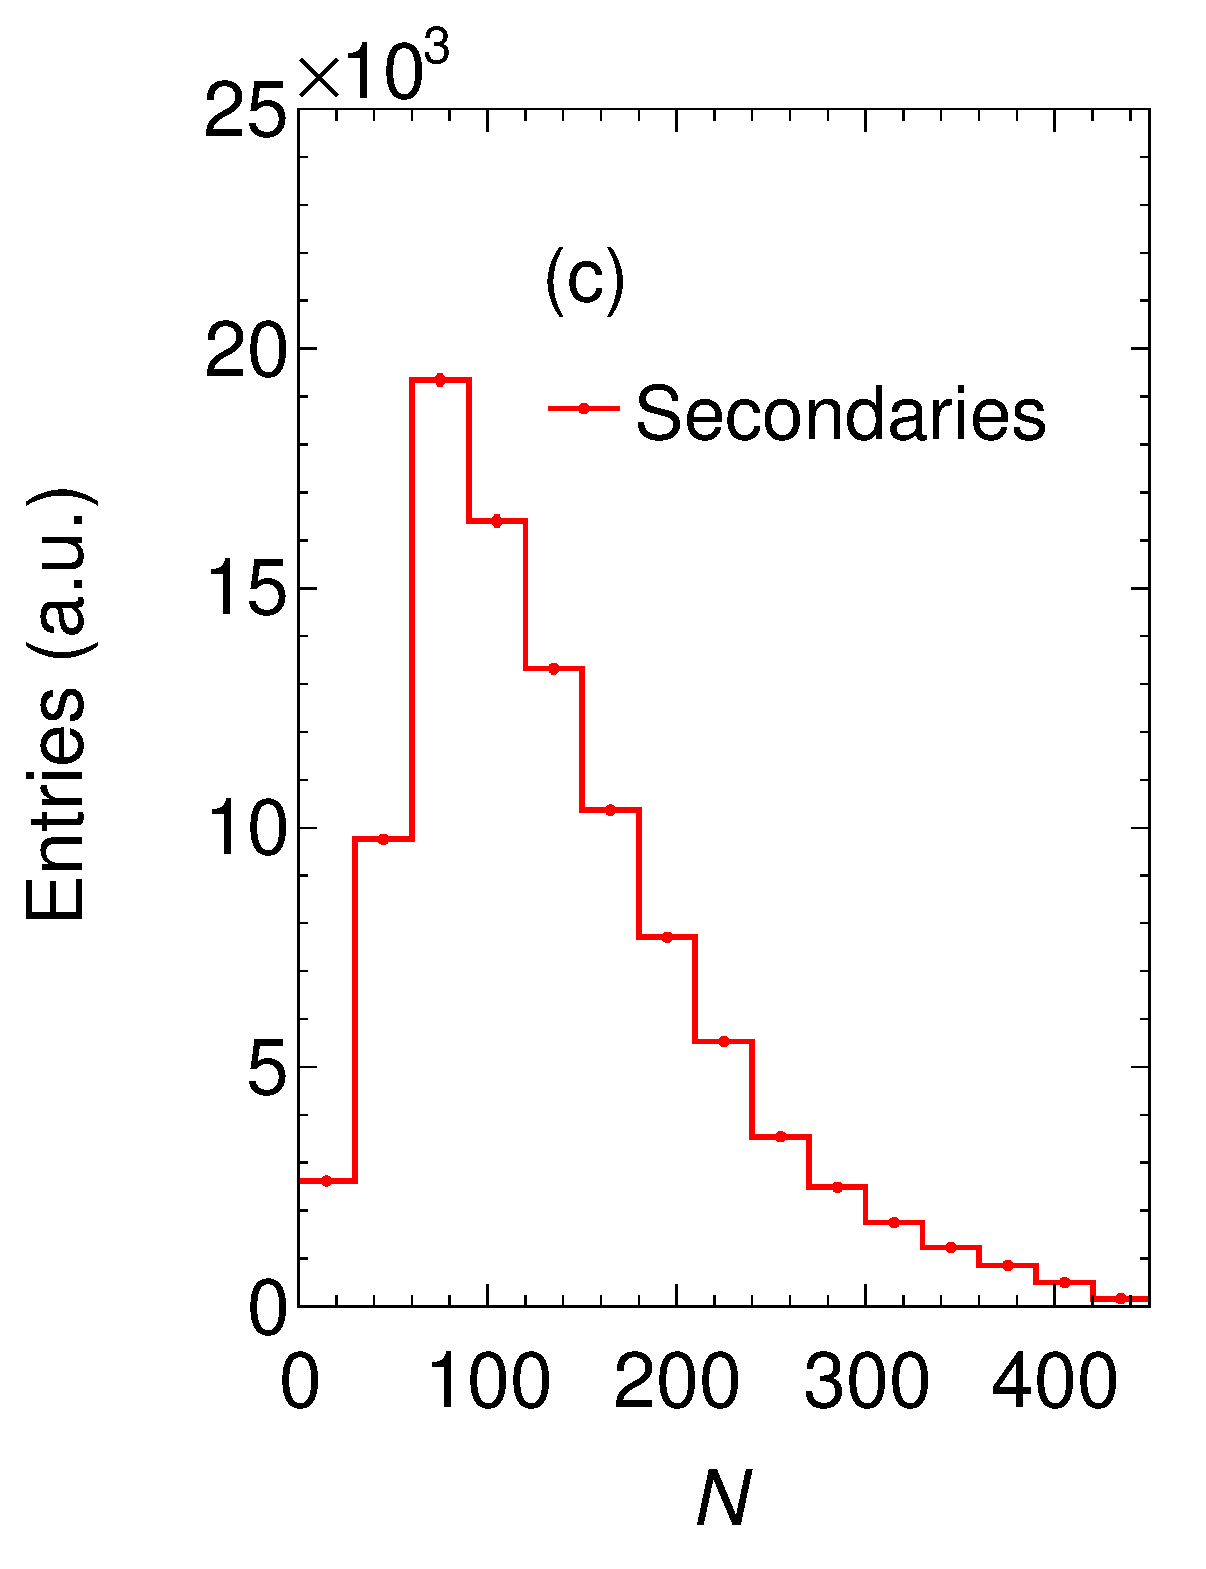
\includegraphics[width=\textwidth]{figures/ch5-KF_NDGAr/ToySample/testNDGArMirrorNAllTall.eps}
         \caption{}
         \label{fig:NGAr}
     \end{subfigure}
        \caption[Distributions of (a) transverse momentum $p_{\textrm{T}}$,  (b) lever arm $L_{\textrm{Arm}}$ and (c) number of points per track $N$ in the HP sample.]{Distributions of (a) transverse momentum $p_{\textrm{T}}$,  (b) lever arm $L_{\textrm{Arm}}$ and (c) number of points per track $N$ in the HP sample. For the HP sample only secondaries are produced, to emulate particles produced in neutrino interactions inside the detector. } \label{fig:GArProperties}
\end{figure}


\subsection{The parameter scan Study}
\label{Sec:ParScan}
The study performed on the PS sample focuses on the validation of the \texttt{Seed} and \texttt{CKF} algorithms as well as on evaluating the improvement in performance produced by the mirroring technique introduced in Sec.~\ref{Sec:KalGAr}. The first test performed on the PS sample was a pull test analogous to what was described in Sec. \ref{Sec:ToyMCTests-Lite}. The pulls $\Pi$ are defined in Eq. \ref{eq:Pull} and can be tested to verify that the diagonal elements of the covariance matrix $C_{ii}$ are well defined. Specifically their distributions should be normal, centered in 0  with $\sigma\simeq1$.

The pulls were tested for the sample, both for the results of the \texttt{Seed} and for the estimates evaluated at the start of the track, after the full propagation of the \texttt{CKF}: the resulting distributions for all the state vector parameters are shown in Figs.~\ref{fig:UnitGAr} and~\ref{fig:UnitGArKF}, respectively. All the pull distributions were fitted to a standard Gaussian distribution and were found to be centered in 0 and have $\sigma\sim1$; this implies that the diagonal elements of the covariance matrices well describe the uncertainties. 

\begin{figure}[!ht]
     \centering
     \begin{subfigure}{0.32\textwidth}
         \centering
         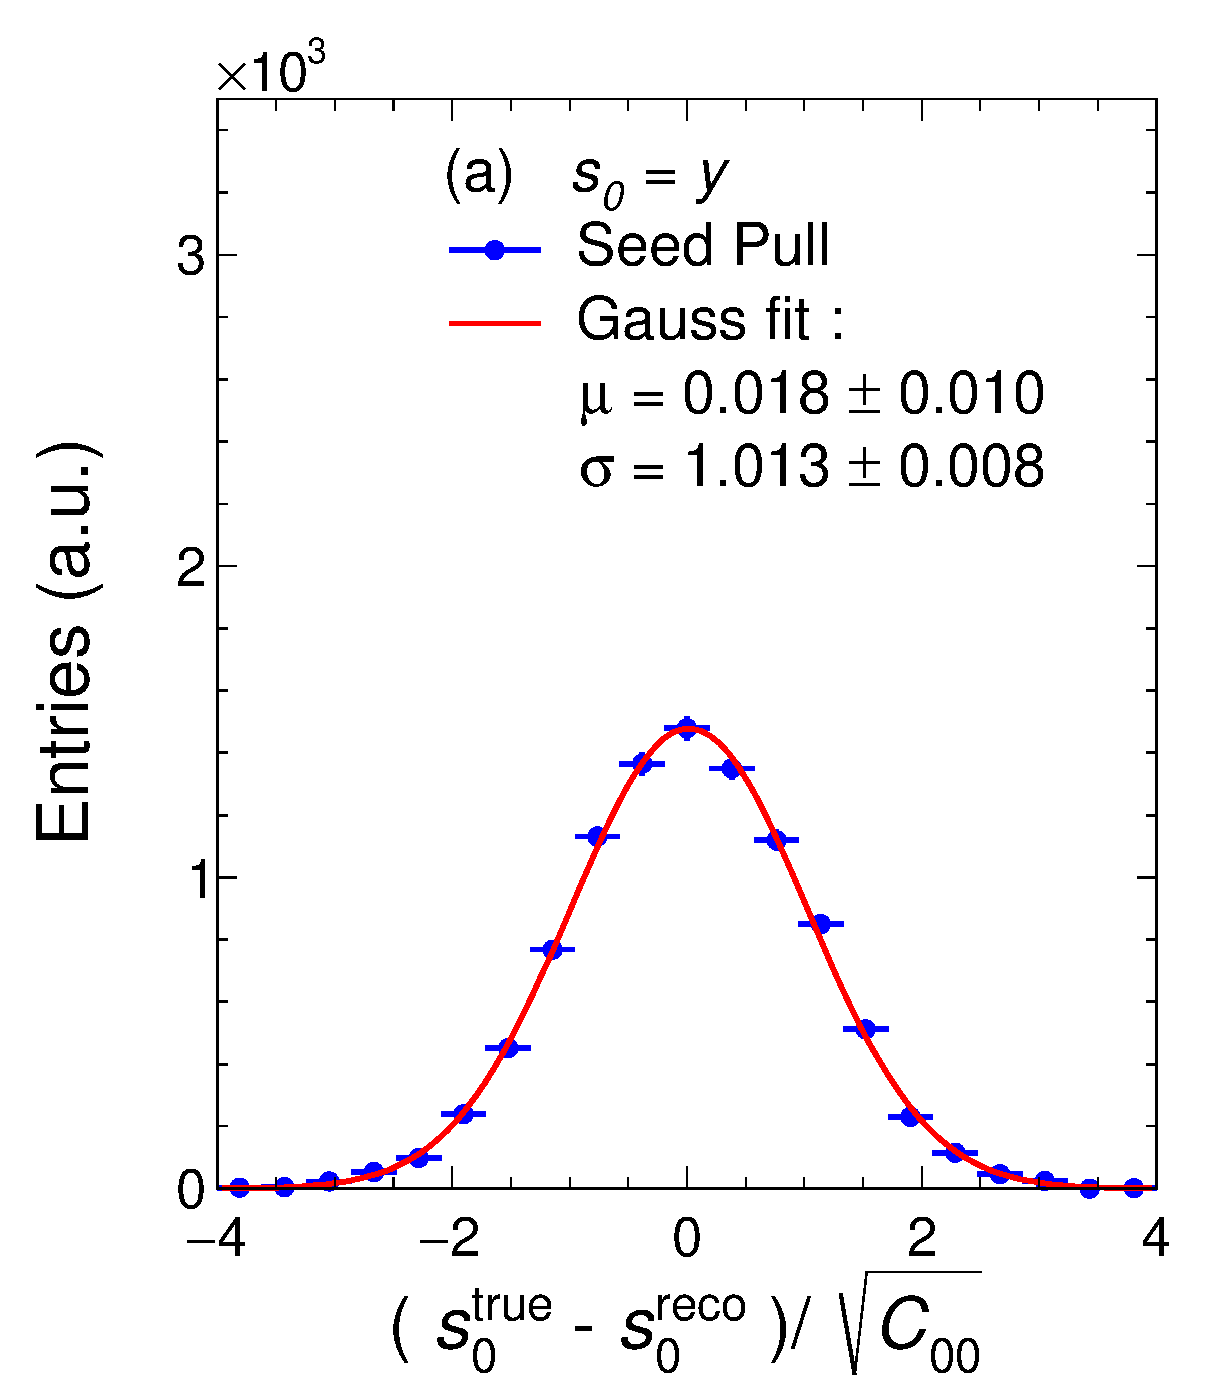
\includegraphics[width=\textwidth]{figures/ch4-KF_NDGArLite/MC/ALICE+KF/UnitSeed_p0.eps}
         \caption{}
         \label{fig:resp0SeedGAr}
     \end{subfigure}
     \begin{subfigure}{0.32\textwidth}
         \centering
         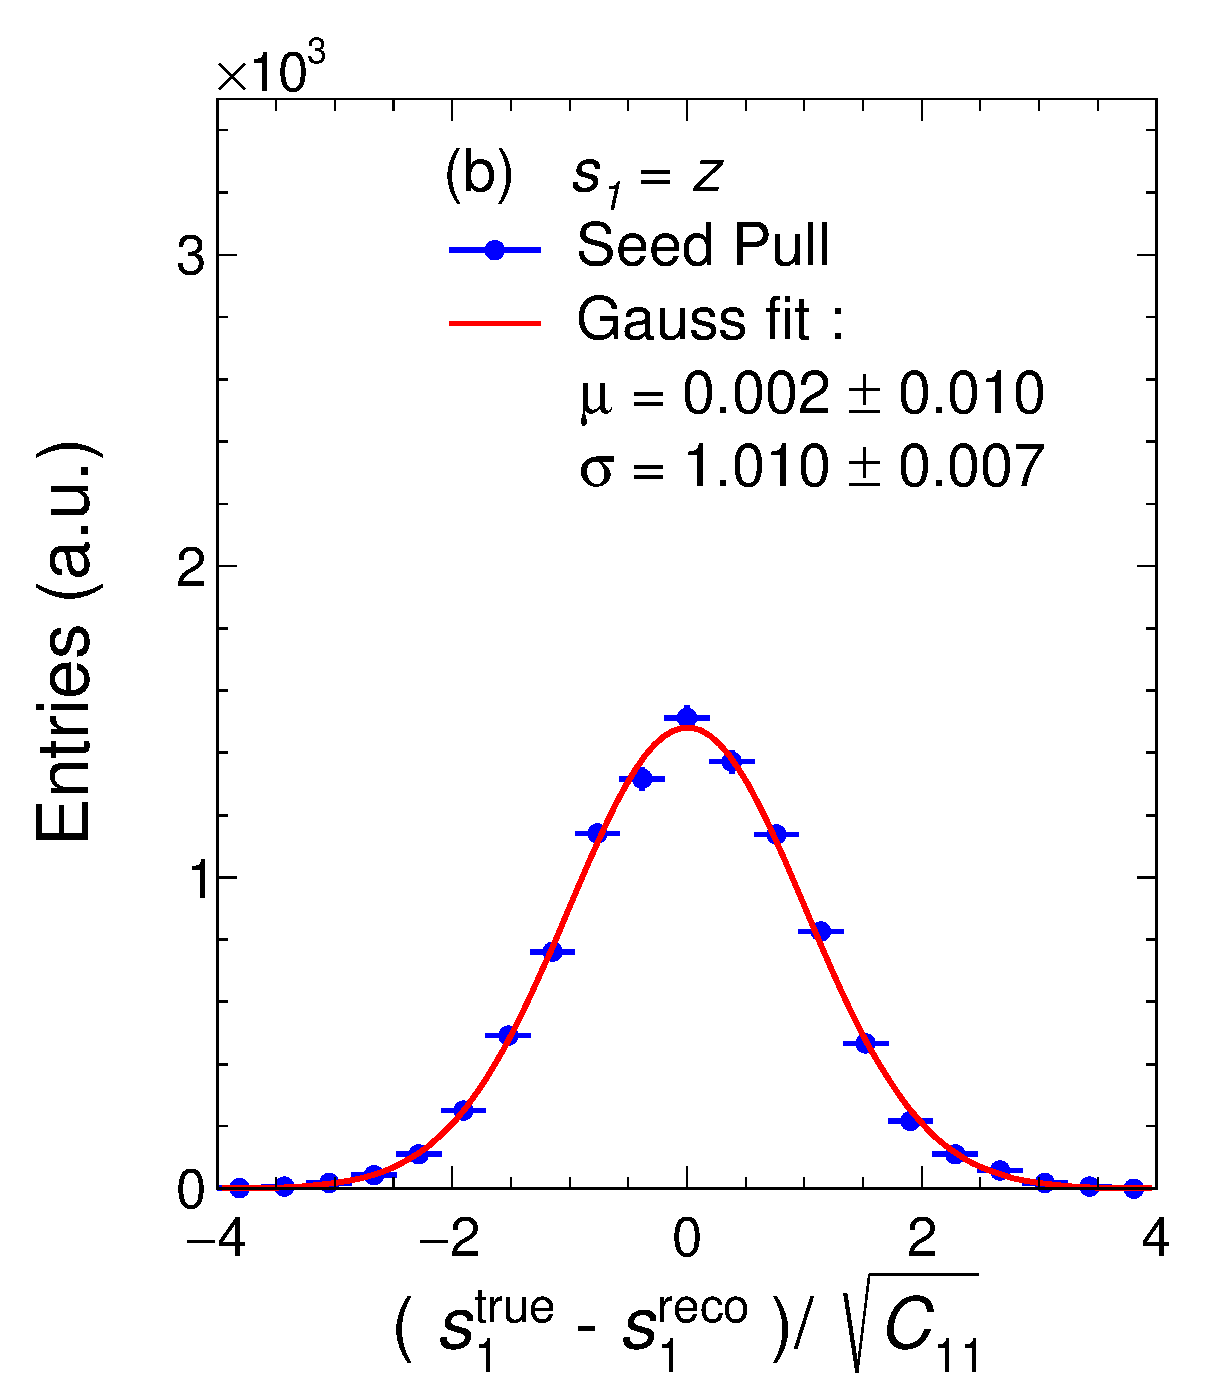
\includegraphics[width=\textwidth]{figures/ch4-KF_NDGArLite/MC/ALICE+KF/UnitSeed_p1.eps}
         \caption{}
         \label{fig:resp1SeedGAr}
     \end{subfigure}
    \begin{subfigure}{0.32\textwidth}
         \centering
         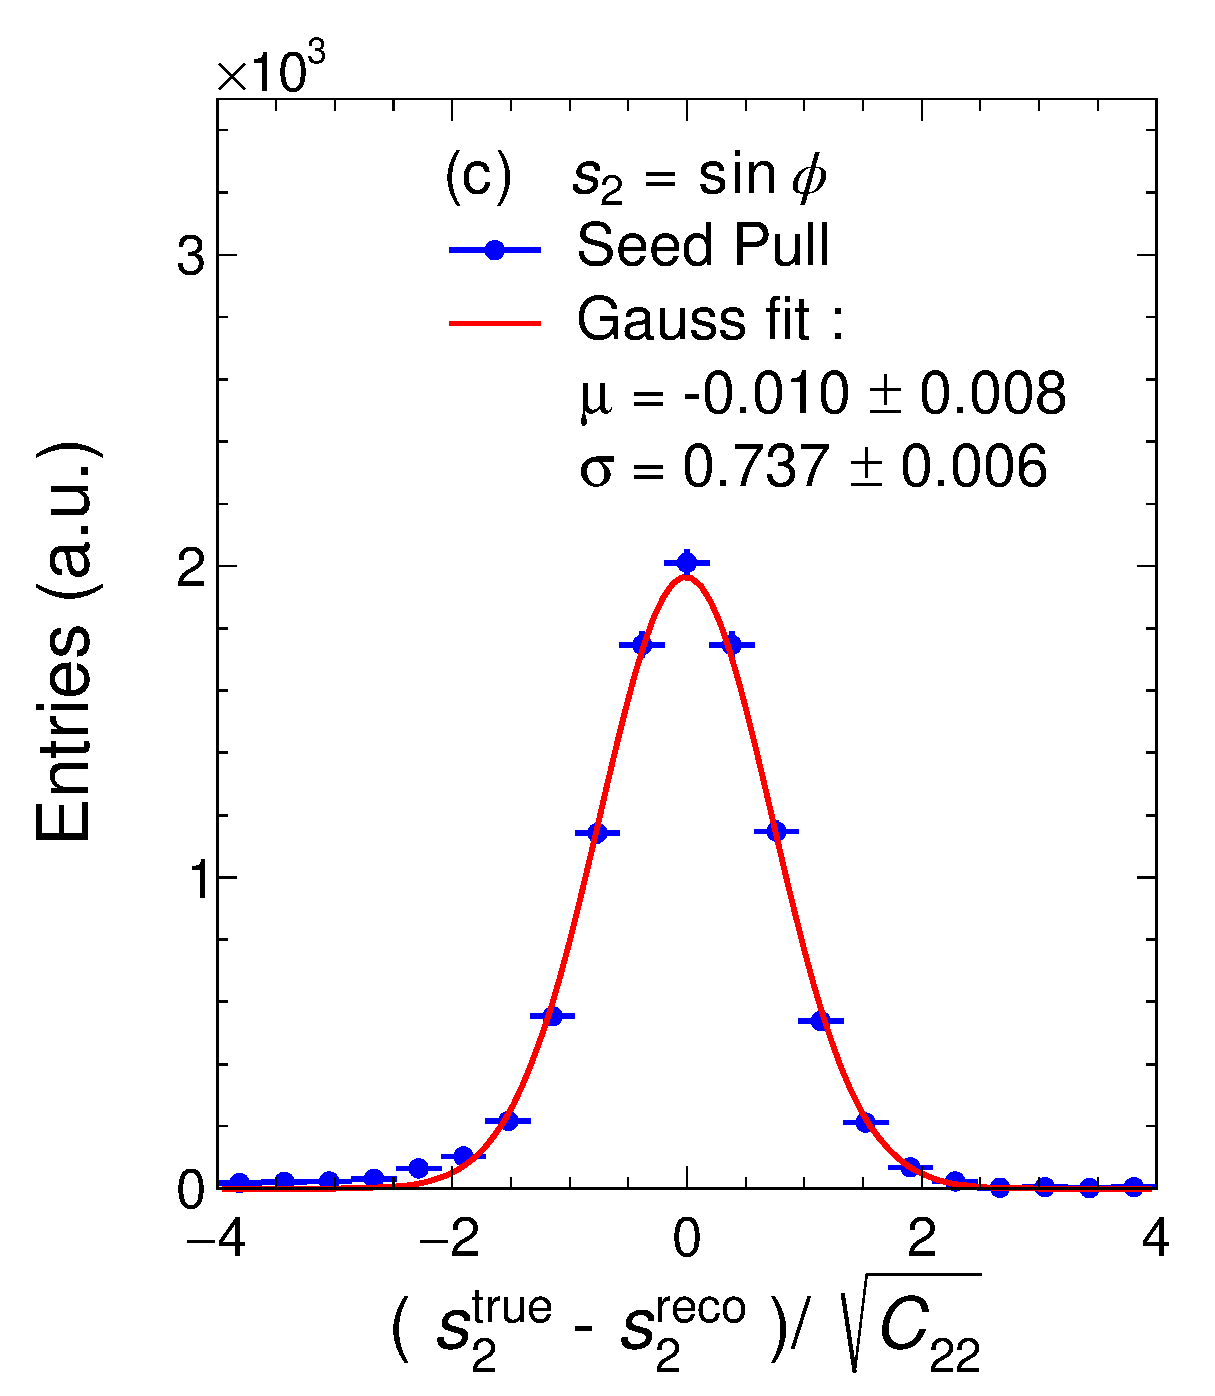
\includegraphics[width=\textwidth]{figures/ch4-KF_NDGArLite/MC/ALICE+KF/UnitSeed_p2.eps}
         \caption{}
         \label{fig:resp2SeedGAr}
     \end{subfigure}
          \begin{subfigure}{0.32\textwidth}
         \centering
         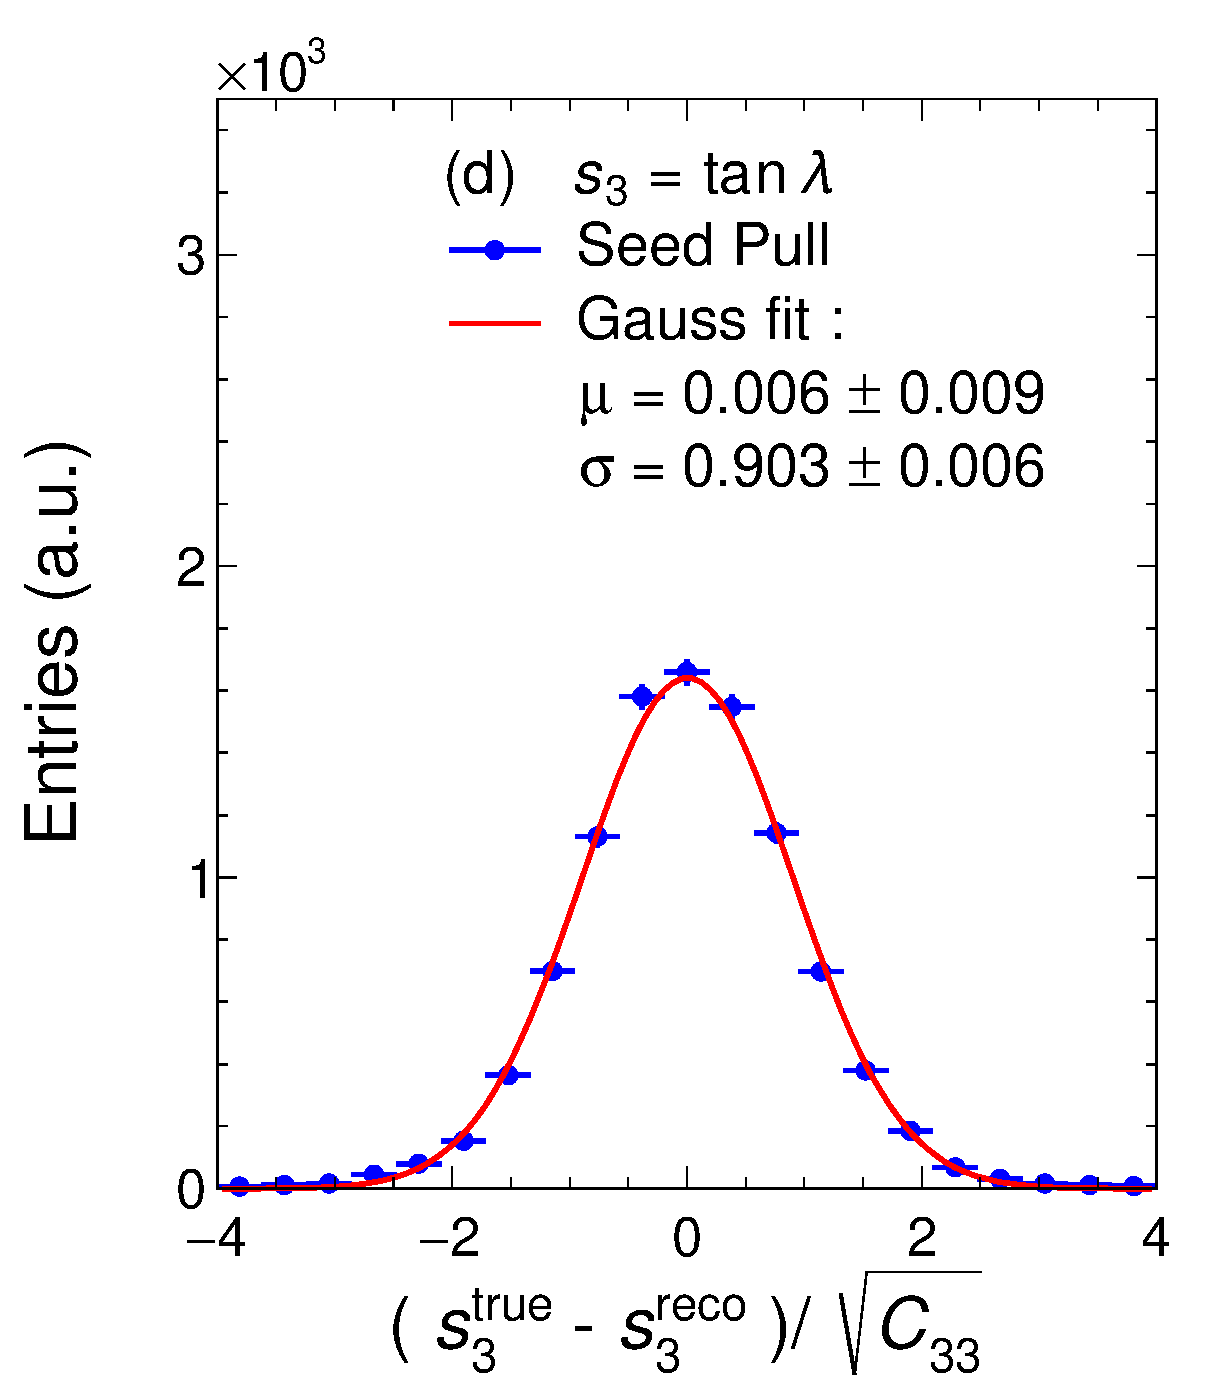
\includegraphics[width=\textwidth]{figures/ch4-KF_NDGArLite/MC/ALICE+KF/UnitSeed_p3.eps}
         \caption{}
         \label{fig:resp3SeedGAr}
     \end{subfigure}
     \begin{subfigure}{0.32\textwidth}
         \centering
         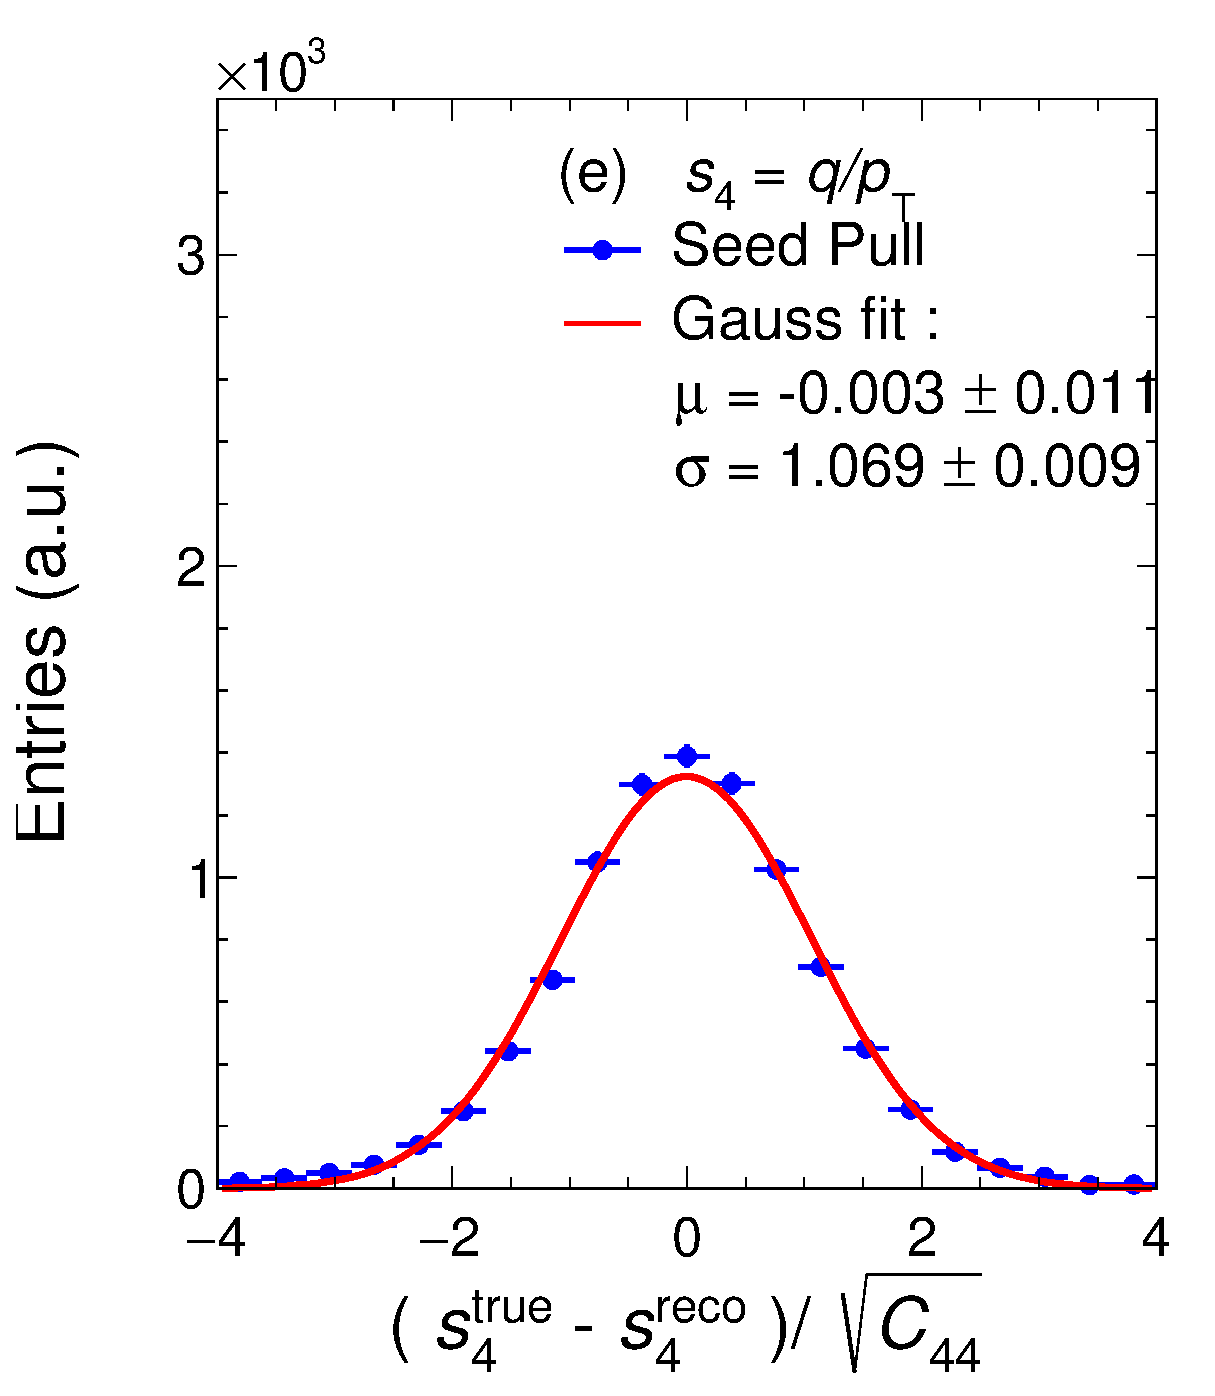
\includegraphics[width=\textwidth]{figures/ch4-KF_NDGArLite/MC/ALICE+KF/UnitSeed_p4.eps}
         \caption{}
         \label{fig:resp4SeedGAr}
     \end{subfigure}
        \caption[Pull distributions for the \texttt{Seed} algorithm over the whole PS sample.]{Pull distributions for the \texttt{Seed} algorithm over the whole PS sample. All distributions were fitted to a Gaussian function. Results for parameters $s_0$ to $s_4$ (i.e. $y$, $x$, $\sin\phi$, $\tan\lambda$ and $q/p_{\text{T}}$) are shown from left to right and labeled from (a) to (e) accordingly. }
        \label{fig:UnitGAr}
\end{figure}

\begin{figure}[!ht]
     \centering
     \begin{subfigure}{0.32\textwidth}
         \centering
         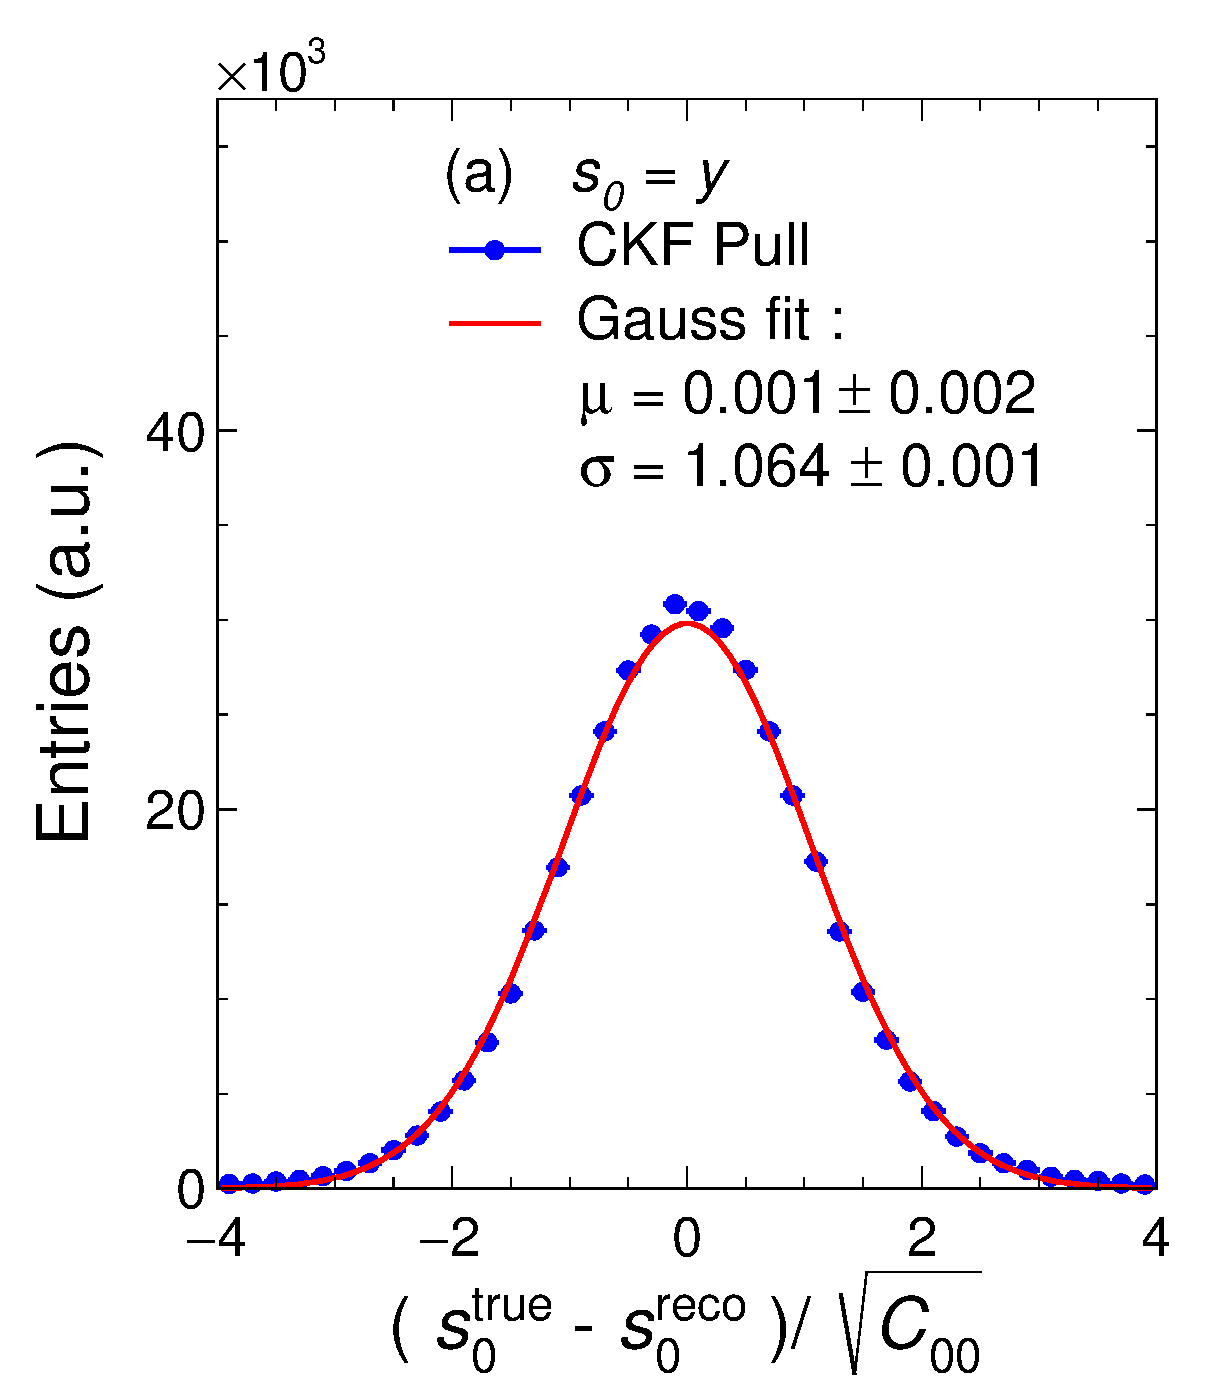
\includegraphics[width=\textwidth]{figures/ch5-KF_NDGAr/ToySample/ParScan/UnitK_p0.eps}
         \caption{}
         \label{fig:resp0KFGAr}
     \end{subfigure}
     \begin{subfigure}{0.32\textwidth}
         \centering
         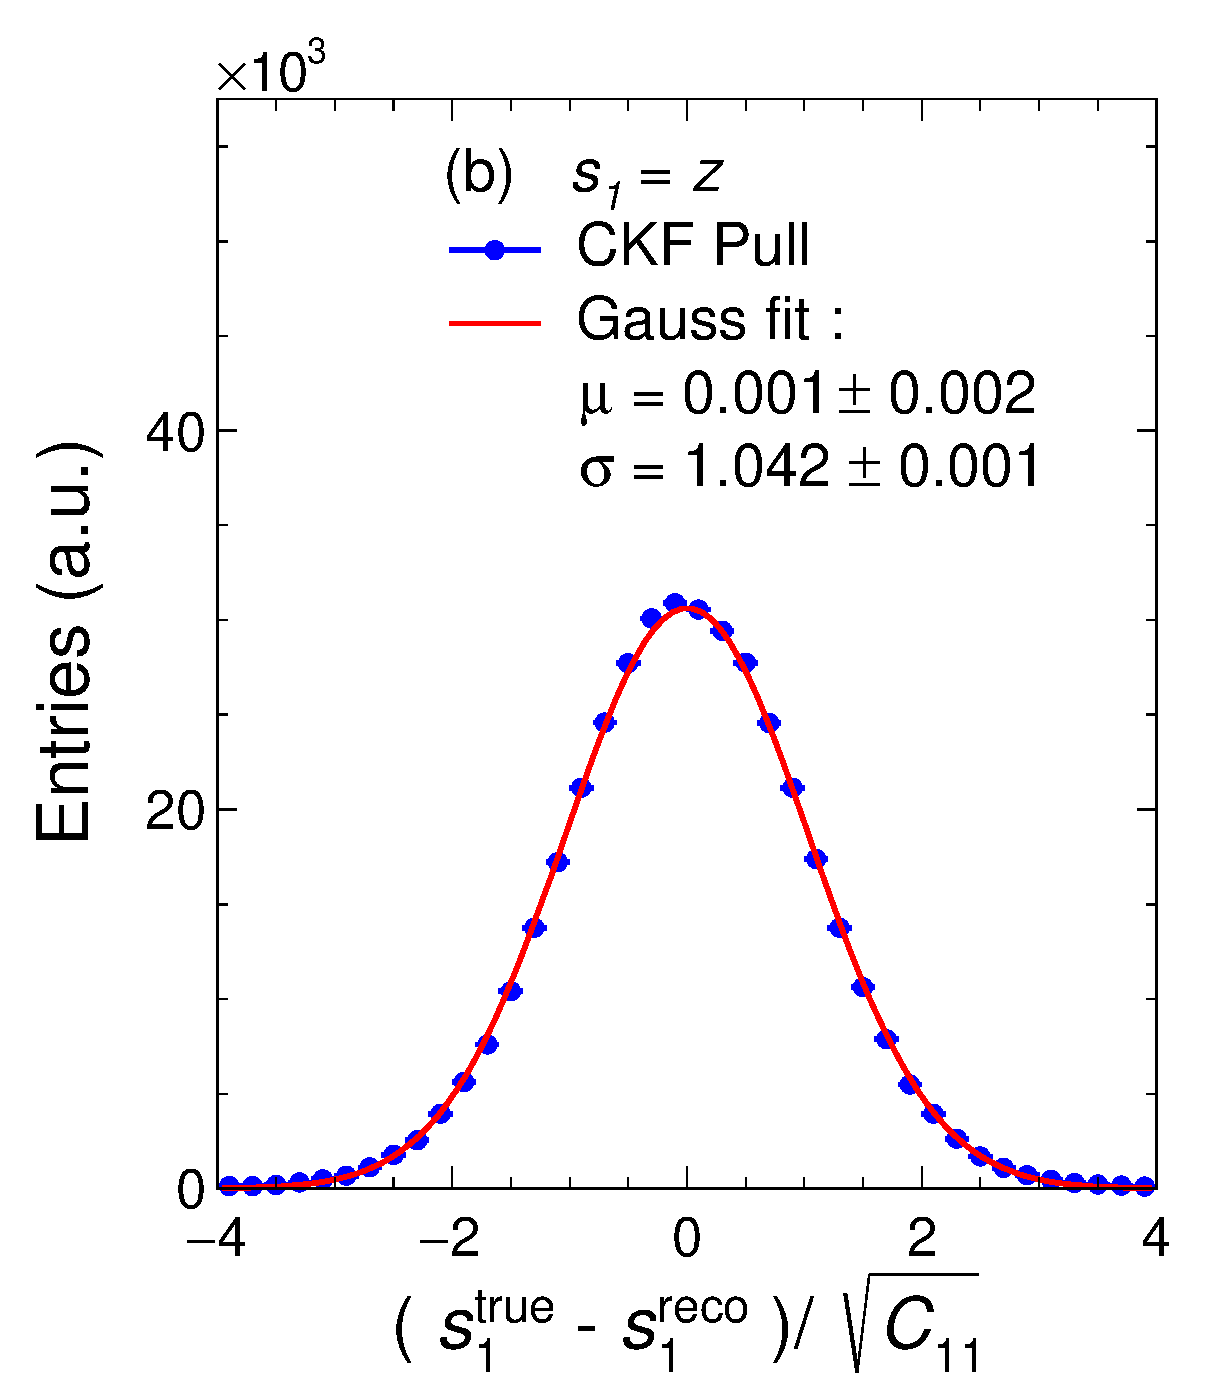
\includegraphics[width=\textwidth]{figures/ch5-KF_NDGAr/ToySample/ParScan/UnitK_p1.eps}
         \caption{}
         \label{fig:resp1KFGAr}
     \end{subfigure}
    \begin{subfigure}{0.32\textwidth}
         \centering
         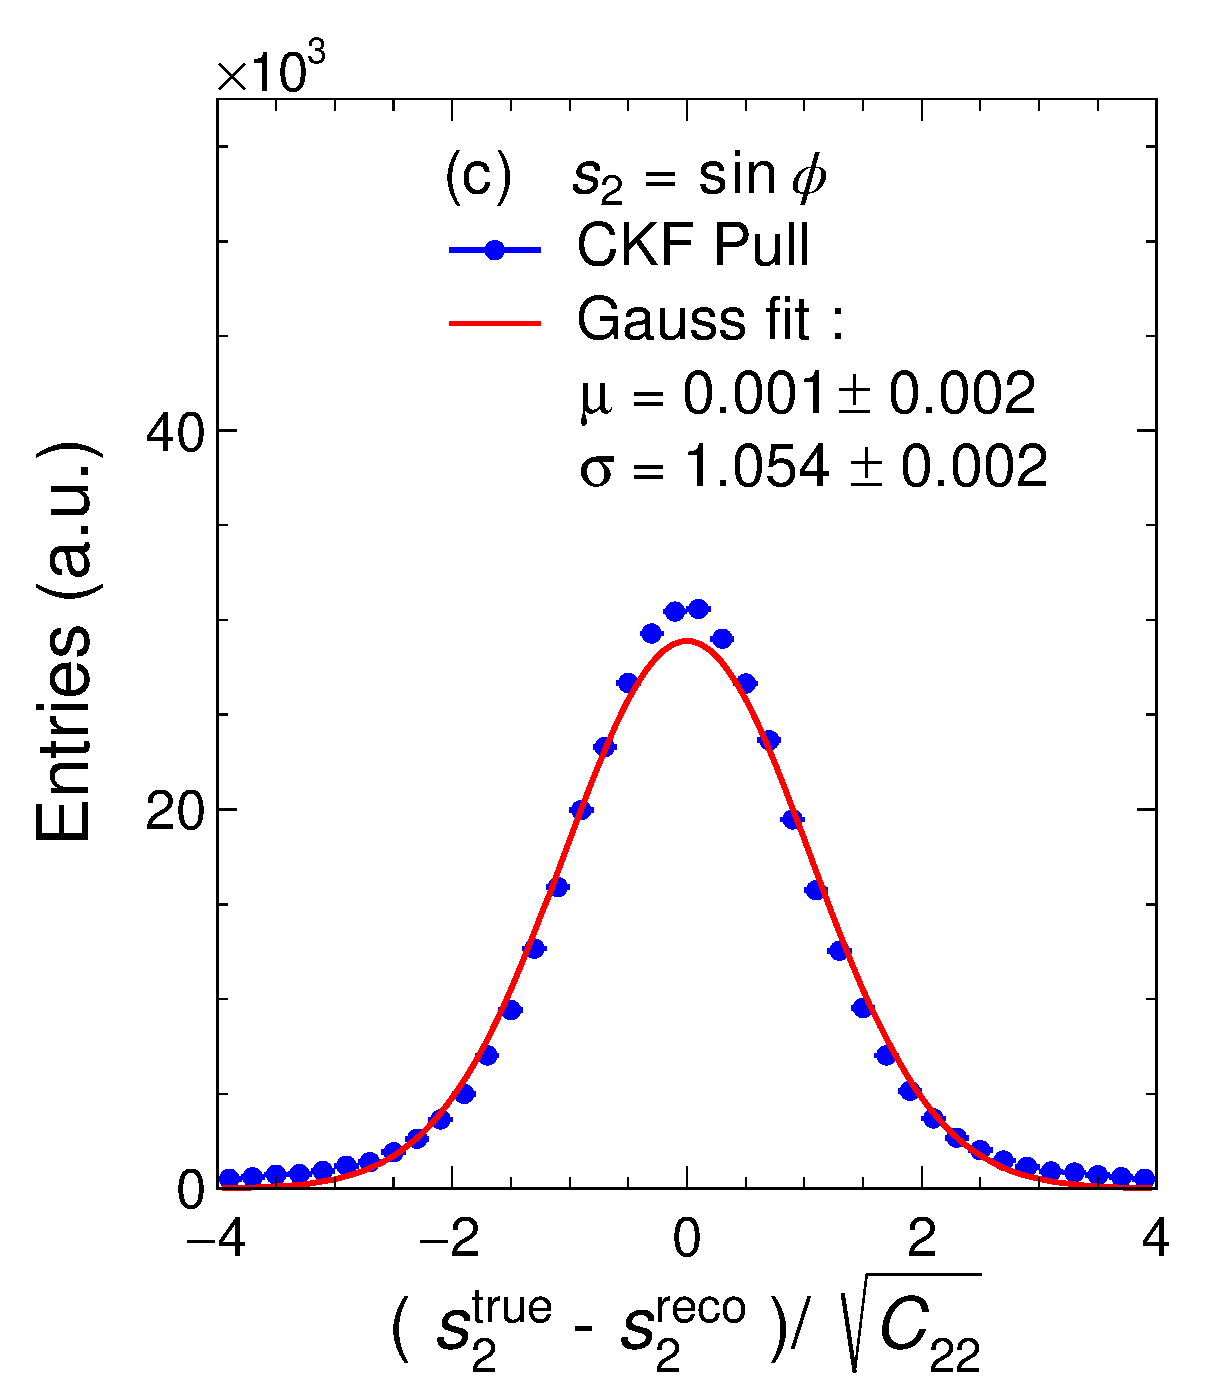
\includegraphics[width=\textwidth]{figures/ch5-KF_NDGAr/ToySample/ParScan/UnitK_p2.eps}
         \caption{}
         \label{fig:resp2KFGAr}
     \end{subfigure}
          \begin{subfigure}{0.32\textwidth}
         \centering
         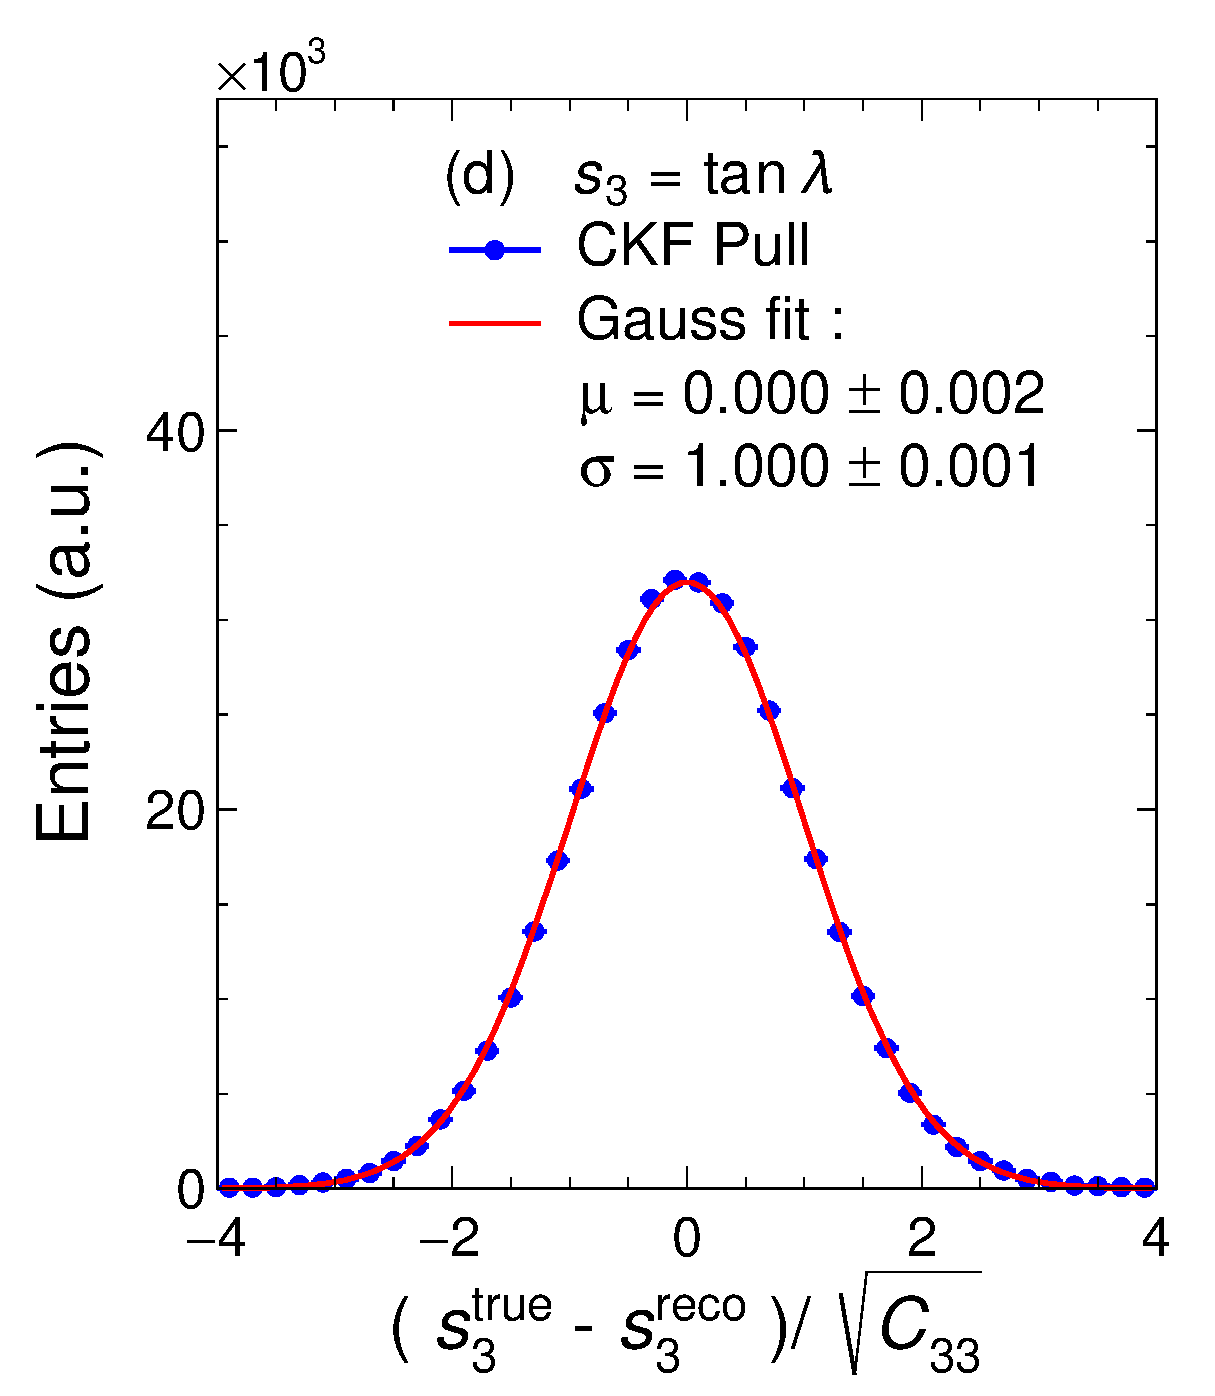
\includegraphics[width=\textwidth]{figures/ch5-KF_NDGAr/ToySample/ParScan/UnitK_p3.eps}
         \caption{}
         \label{fig:resp3KFGAr}
     \end{subfigure}
     \begin{subfigure}{0.32\textwidth}
         \centering
         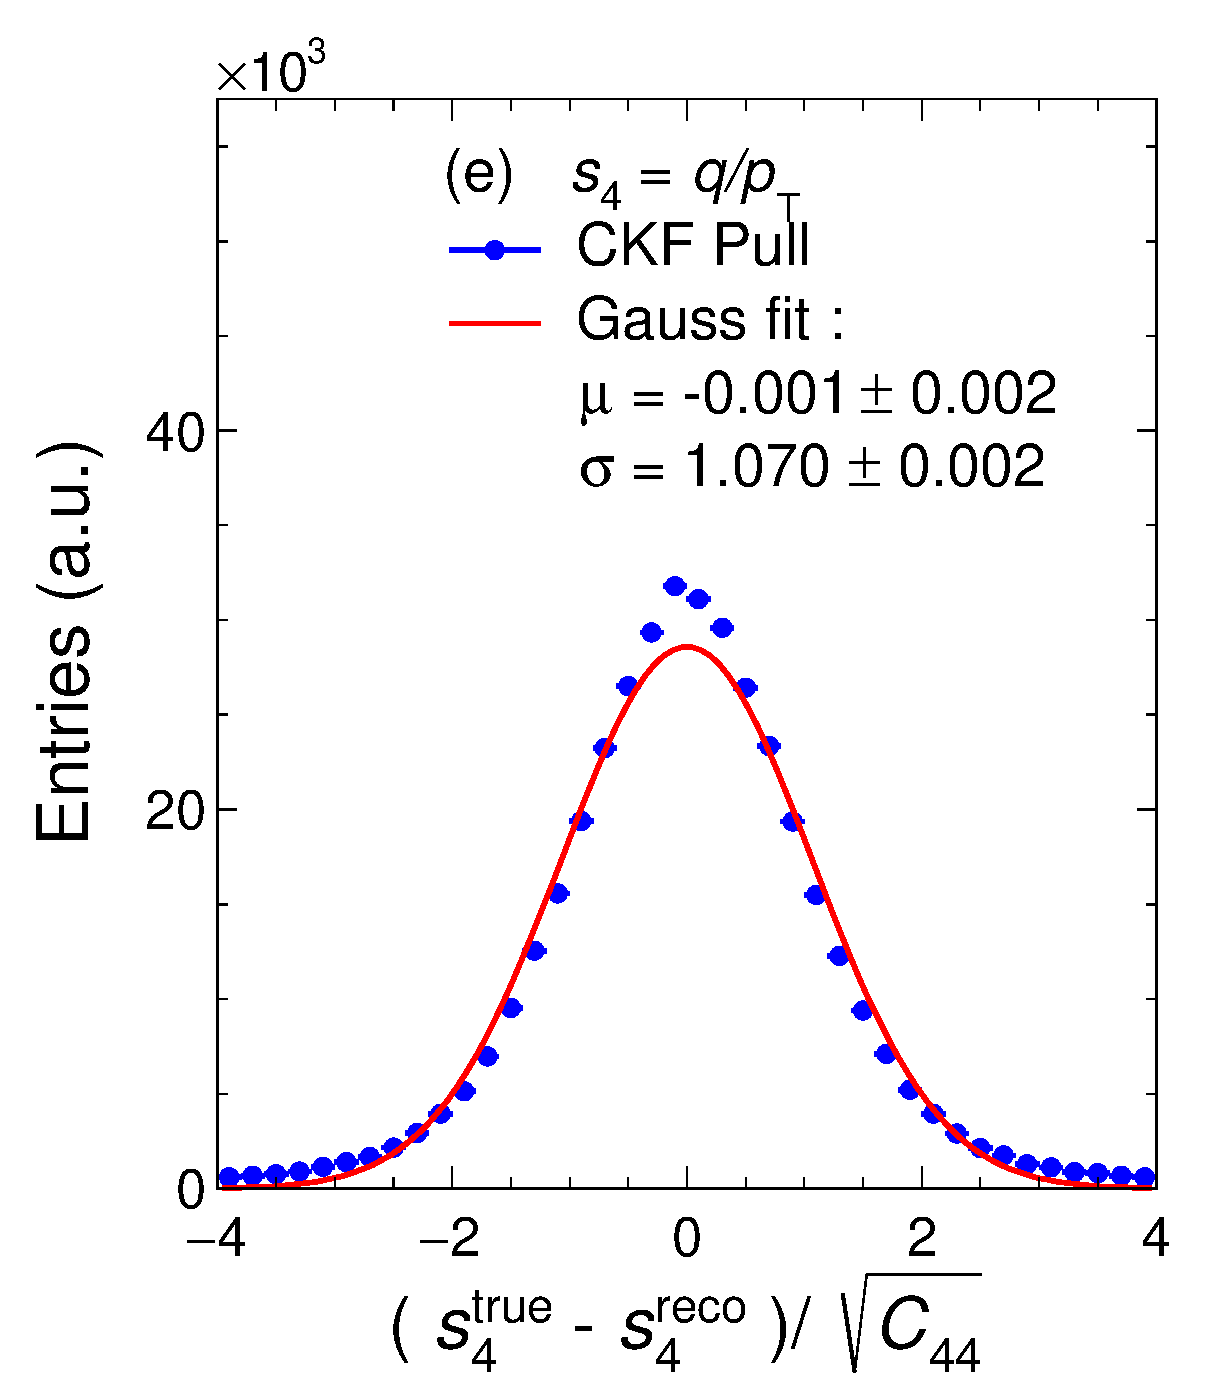
\includegraphics[width=\textwidth]{figures/ch5-KF_NDGAr/ToySample/ParScan/UnitK_p4.eps}
         \caption{}
         \label{fig:resp4KFGAr}
     \end{subfigure}
        \caption[Pull distributions obtained after the full propagation of the \texttt{CKF} algorithm over the whole PS sample.]{Pull distributions obtained after the full propagation of the \texttt{CKF} algorithm over the whole PS sample. See Fig.~\ref{fig:UnitGAr} for comparison.}
        \label{fig:UnitGArKF}
\end{figure}

The standard pull distributions, while being effective at testing the uncertainties associated with the individual parameters, do not provide any information regarding the off-diagonal correlation terms. In order to test the quality of the estimates for the full covariance matrix, the Mahalanobis distance was used~\cite{M-distance}. Given a probability distribution, $D$, on $\mathbb{R}^n$ with mean $\mu$ and positive-definite covariance matrix, $C$, the Mahalanobis distance, $M$, of a point $s$ from $D$, is defined as:
\begin{equation}
    M = \sqrt{(s-\mu)^TC^{-1}(s-\mu)},
\end{equation}
where in our case, $\mu$ corresponds to the true value of state vector, $s^{\text{true}}$, $s$ and $C$ are the estimates obtained from the reconstruction and $n=5$. The Mahalanobis distance, $M$, of a set of points belonging to the distribution $D$, follows a $\chi^2$ distribution with $n$ degrees of freedom. One can check if $C$ is well defined, by verifying that the corresponding $M$ follow a $\chi^2$ distribution with the correct number of degrees of freedom. In Fig.~\ref{fig:chi2}, we show the results of a $\chi^2$ fit over the $M$ distribution for the whole sample. The plot on the left shows the results obtained from the \texttt{Seed} algorithm, while the one on the right shows the results after the full \texttt{CKF} propagation. In both cases the n.d.f. obtained with the $\chi^2$ fit are very close to $n=5$: both \texttt{Seed} and \texttt{CKF} estimates accurately the covariances of the reconstructed track parameters in the state vector. 


\begin{figure}[!ht]
     \centering
     \begin{subfigure}[b]{0.48\textwidth}
         \centering
         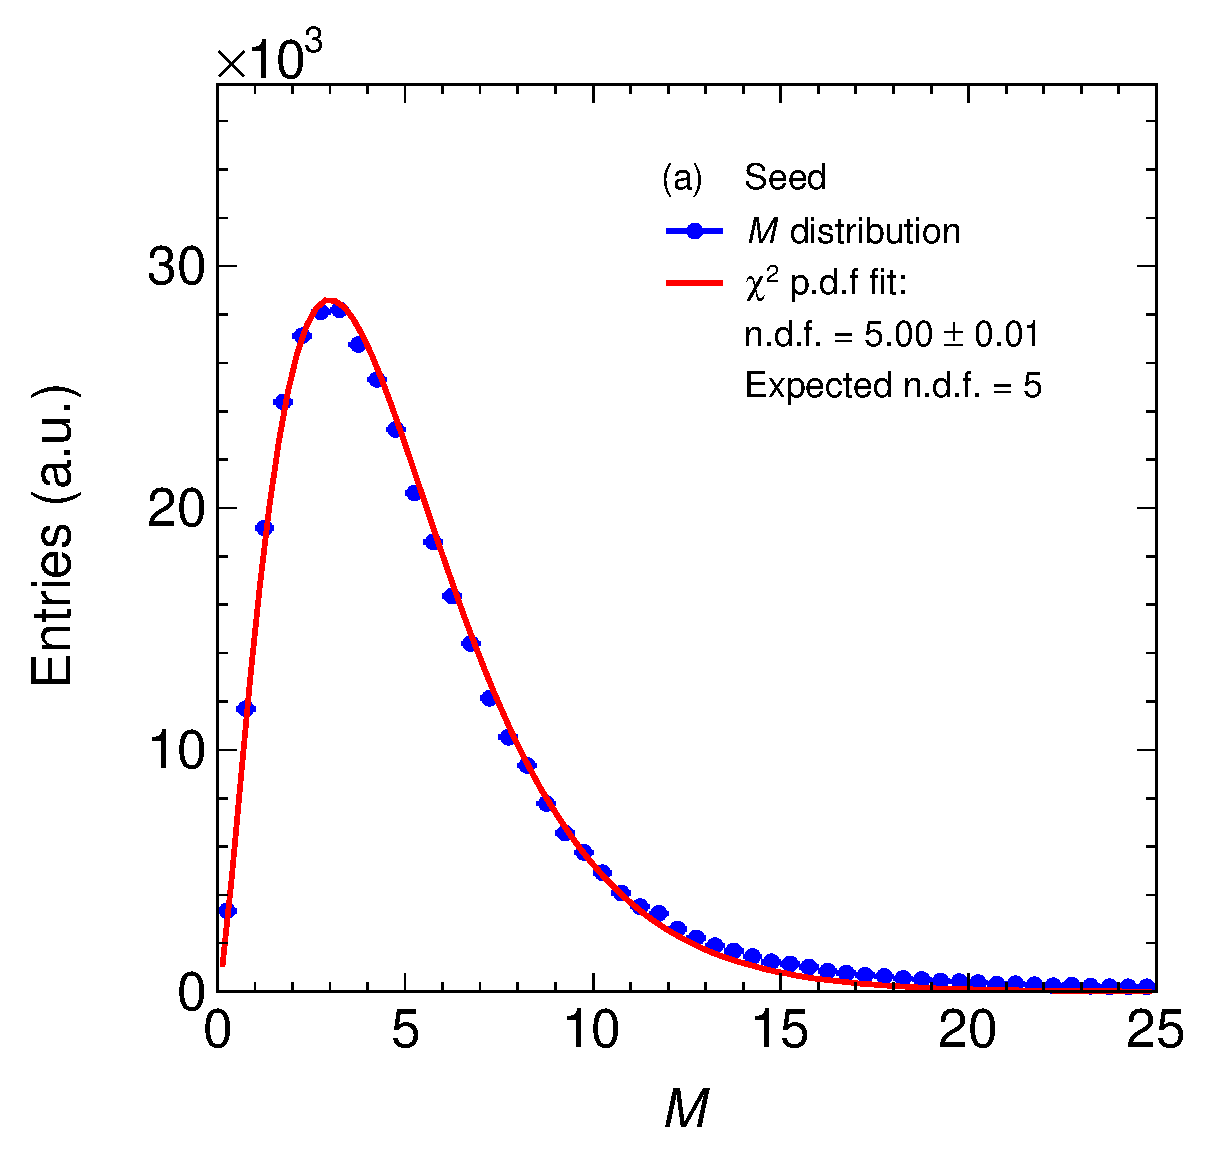
\includegraphics[width=\textwidth]{figures/ch5-KF_NDGAr/ToySample/ParScan/MDistanceSeed.eps}
         \caption{}
         \label{fig:chi2Seed}
     \end{subfigure}
     \begin{subfigure}[b]{0.48\textwidth}
         \centering
         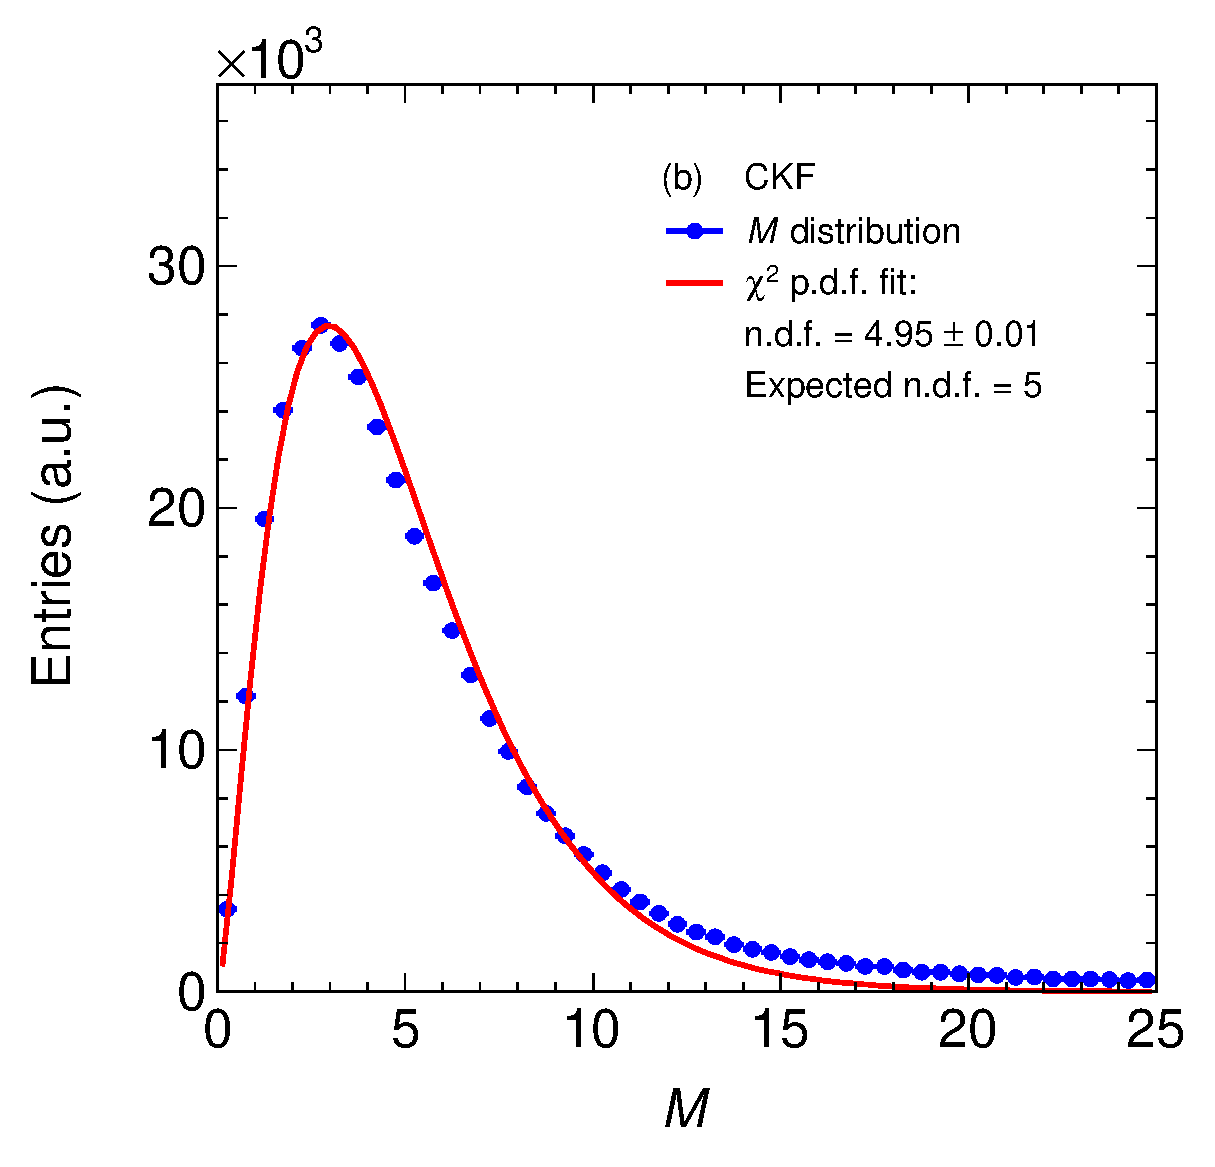
\includegraphics[width=\textwidth]{figures/ch5-KF_NDGAr/ToySample/ParScan/MDistanceKalman.eps}
         \caption{}
         \label{fig:chi2Kalman}
     \end{subfigure}
        \caption[Mahalanobis distance $M$ distribution for the PS Sample.]{Mahalanobis distance $M$ distribution for the PS Sample fitted by a standard $\chi^2$ p.d.f. showing the results for the $n.d.f.$ parameter. The expected result for a 5-dimensional matrix is $n.d.f. = 5$. The results for the \texttt{Seed} and for the fully propagated \texttt{CKF} are shown in plots (a) and (b) respectively. } \label{fig:chi2}
\end{figure}


The PS sample was also used to test whether the \texttt{CKF} algorithm produced results that are consistent with the theoretical expectations. The analytical formula for the ideal $q/p_{\text{T}}$ resolution, $\sigma_{\text{theo}}(q/p_{\text{T}})=\sqrt{C_{44}^{\textrm{theo}}}$, obtainable using a curvature measurement in a TPC, can be written analogously to what was shown for the total momentum in Eqs. \ref{eq:sigmaNptot} and \ref{eq:sigmaMSptot} as~\cite{PDG:34,Gluckstern:1963}:
\begin{equation}
   \sigma_{\text{theo}}(1/p_{\text{T}}) = \sqrt{C_{44}^{\textrm{theo}}} = \sqrt{\sigma_{\text{H}}^2+\sigma_{\text{MS}}^2}.
\end{equation}
The $\sigma_{\text{H}}$ component is determined by the point resolution and can be written as:
\begin{equation}\label{eq:sigmaN}
    \sigma_{\text{H}}(1/p_{\text{T}})=\frac{\sigma_{r\phi}}{0.3BL_{\textrm{Arm}}^2}\sqrt{\frac{720}{N+4}}.
\end{equation} 
The multiple scattering component can be written as:
\begin{equation}\label{eq:sigmaMS}
    \sigma_{\text{MS}}(1/p_{\text{T}})=\bigg\langle\frac{1}{\beta p_{\text{T}}}\bigg\rangle\frac{0.016 \ (\textrm{GeV}/c)}{0.3 B l\cos\lambda}\sqrt{\frac{l}{X_0}},
\end{equation}
where $l$ is the length of the track in the $xy$-plane. 
Note that the value of $1/\left(\beta p_{\text{T}}\right)$ is averaged along the trajectory to take into account energy loss. In Figs.~\ref{fig:Check_Ana_pID},~\ref{fig:CheckAna_dens} and~\ref{fig:Check_Ana_res},  the upper plots show the \texttt{CKF} covariance estimates, $\sqrt{C_{44}^{\textrm{CKF}}}$, while the bottom plots show their ratios to the theoretical expectations, $\sqrt{C_{44}^{\textrm{theo}}}$. The points analyzed are randomly taken along the reconstructed tracks and down-sampled to $10\%$ of the total to avoid correlations.

\begin{figure}[!ht]
     \centering
     \begin{subfigure}[b]{0.99\textwidth}
         \centering
         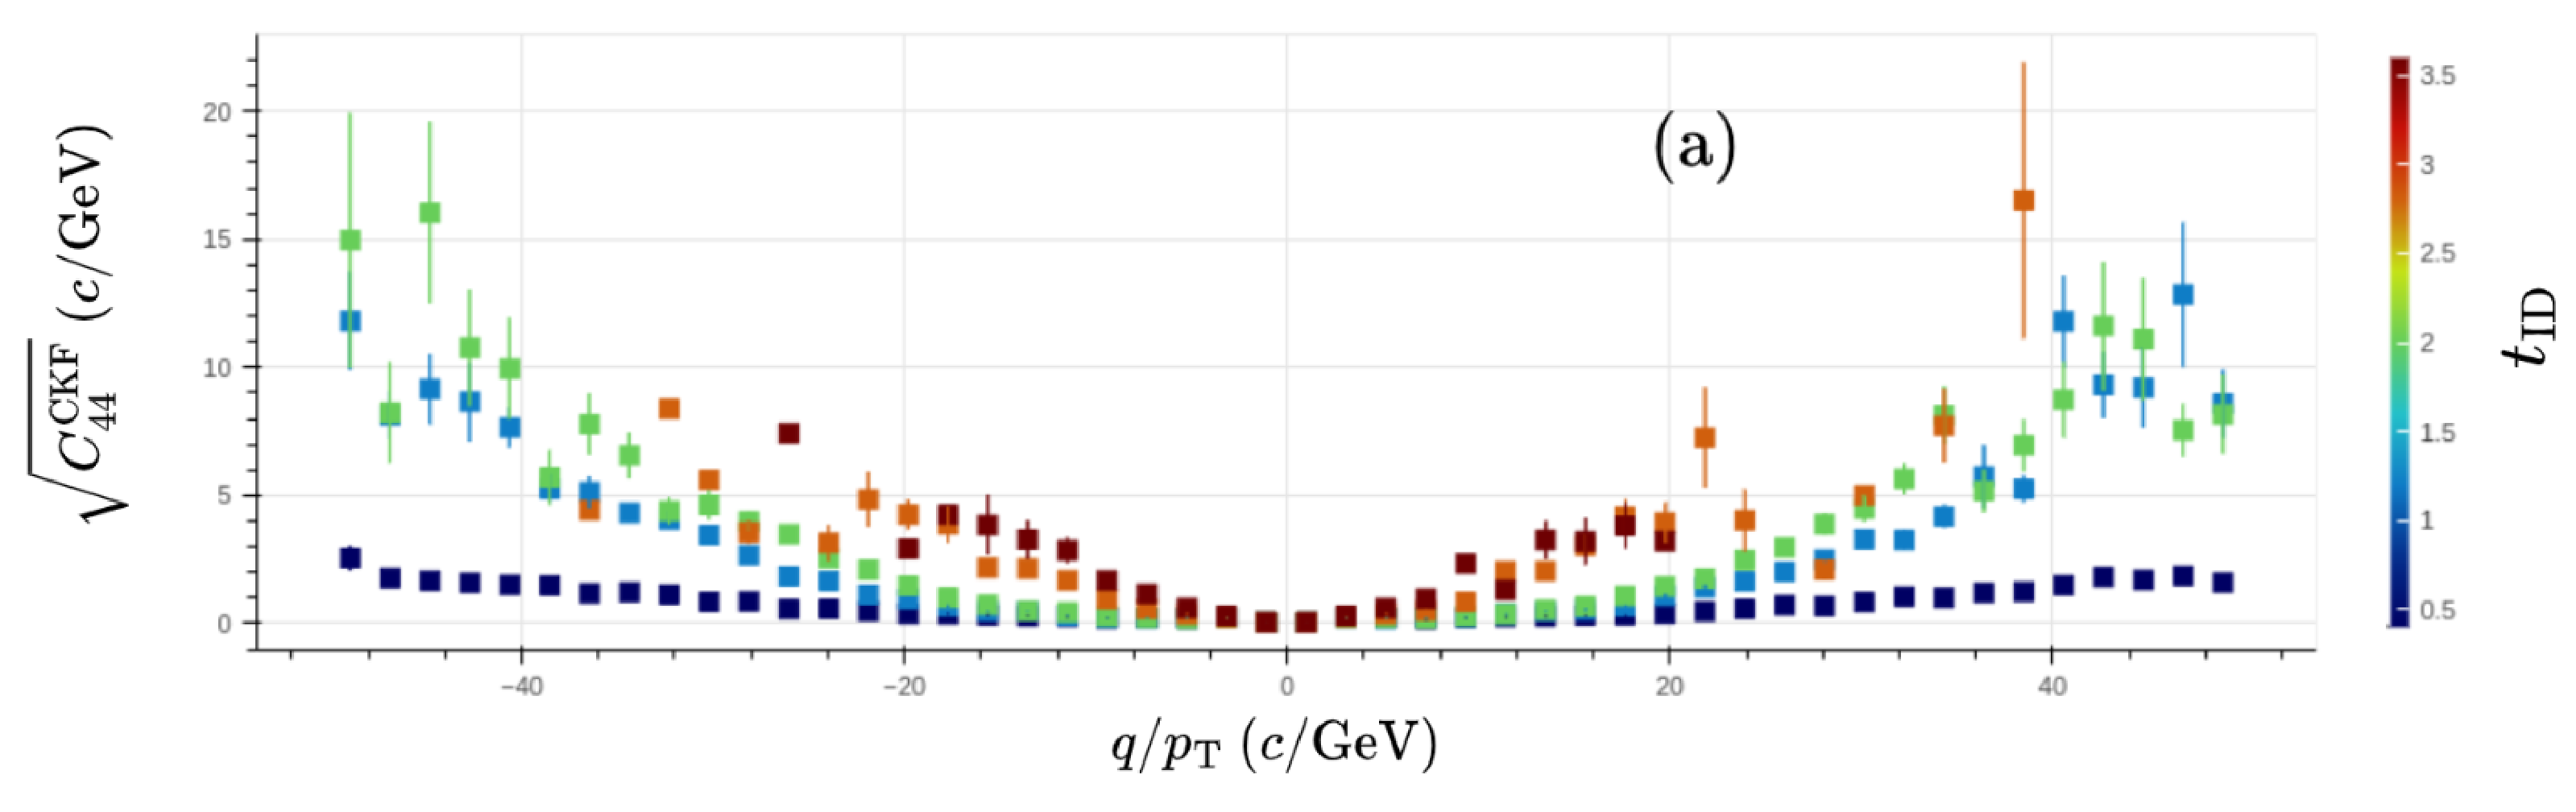
\includegraphics[width=\textwidth]{figures/ch5-KF_NDGAr/ToySample/ParScan/TotVSExpVSpID_noNorm_label.eps}
         \caption{}
         \label{fig:CheckAna_pID_noNorm}
     \end{subfigure}
     \begin{subfigure}[b]{0.99\textwidth}
         \centering
         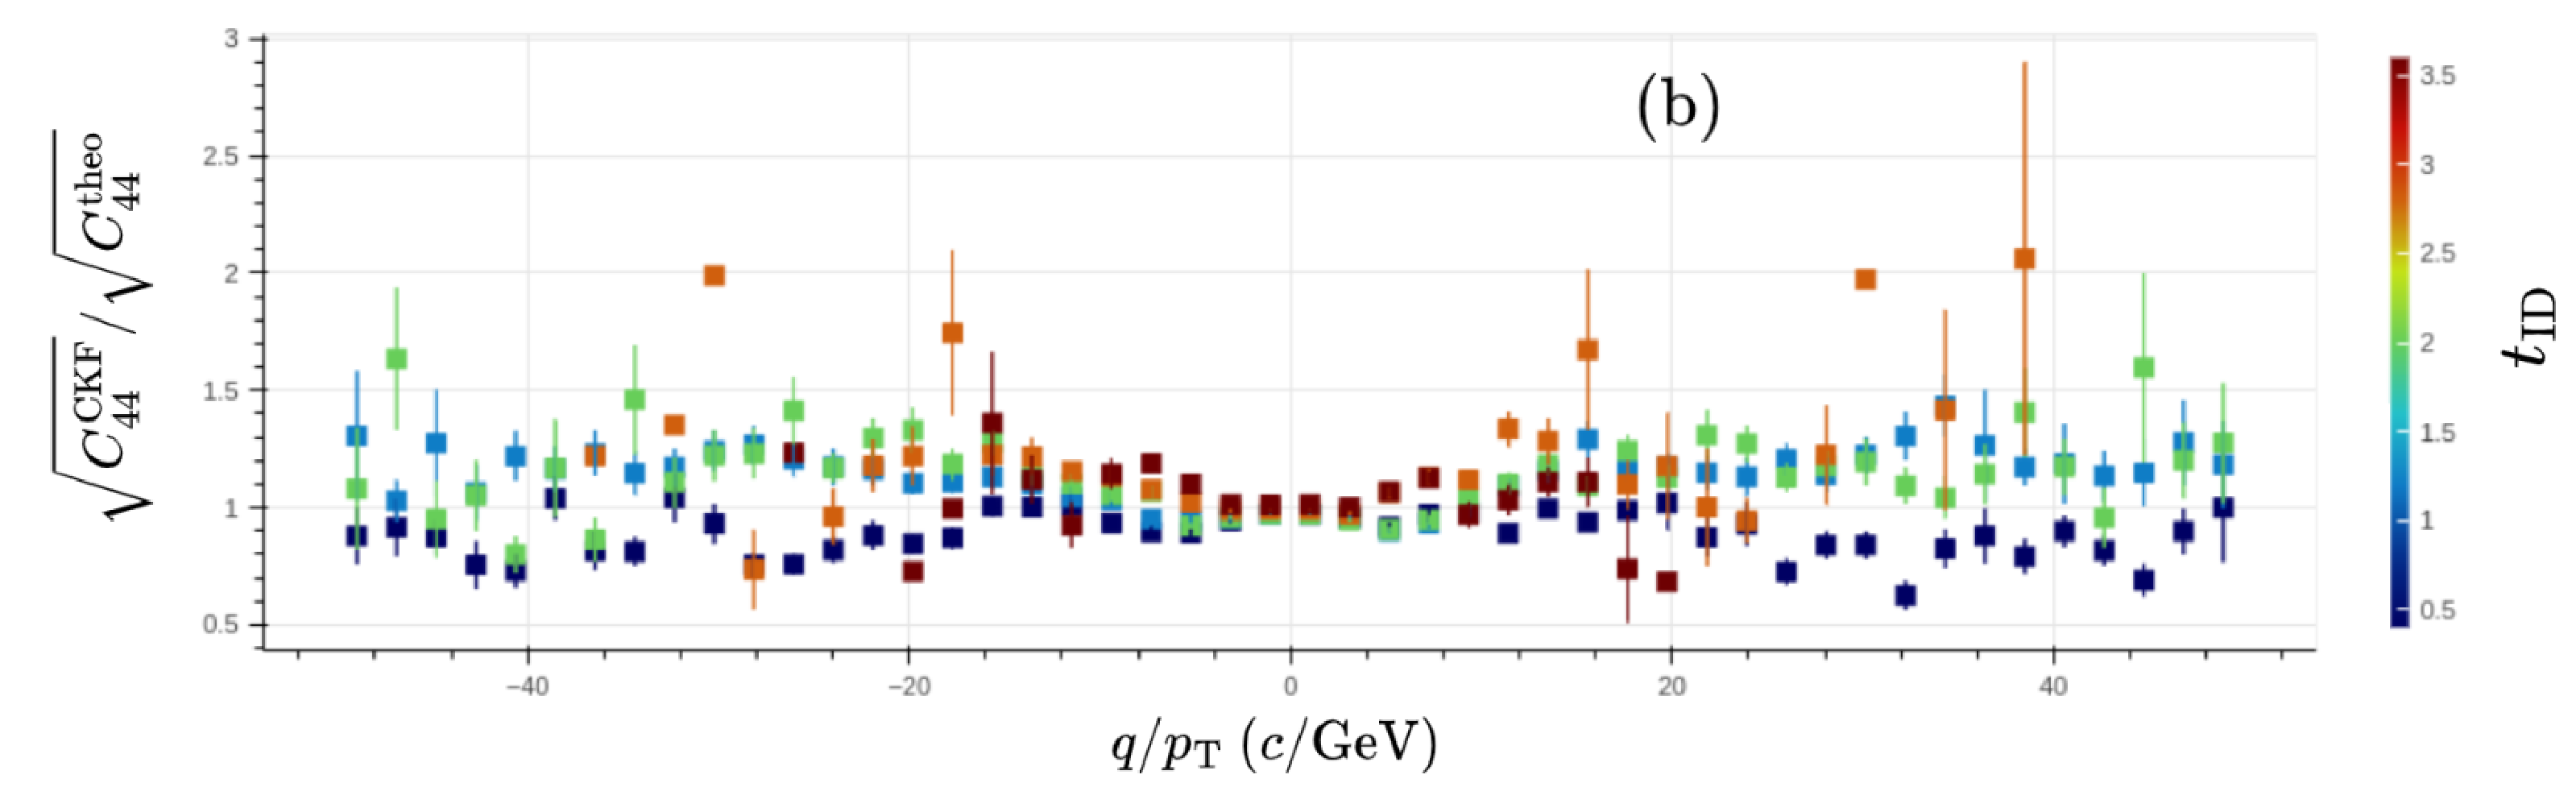
\includegraphics[width=\textwidth]{figures/ch5-KF_NDGAr/ToySample/ParScan/TotVSExpVSpID_label.eps}
         \caption{}
         \label{fig:CheckAna_pID_Norm}
     \end{subfigure}
        \caption[(a) \texttt{CKF} $q/p_{\text{T}}$ resolution $\sigma_{\text{CKF}}(q/p_{\text{T}})=\sqrt{C_{44}^{\textrm{CKF}}}$ as a function of the true $q/p_{\text{T}}$. (b) Ratio of the \texttt{CKF} $q/p_{\text{T}}$ resolution, over the theoretical expectations $\sigma_{\text{theo}}(q/p_\text{T})=\sqrt{C_{44}^{\textrm{theo}}}$, as a function of the true $q/p_\text{T}$.]{ (a) \texttt{CKF} $q/p_{\text{T}}$ resolution $\sigma_{\text{CKF}}(q/p_{\text{T}})=\sqrt{C_{44}^{\textrm{CKF}}}$ as a function of the true $q/p_{\text{T}}$. (b) Ratio of the \texttt{CKF} $q/p_{\text{T}}$ resolution, over the theoretical expectations $\sigma_{\text{theo}}(q/p_\text{T})=\sqrt{C_{44}^{\textrm{theo}}}$, as a function of the true $q/p_\text{T}$. The histograms include all particles in the PS sample and are color-coded according to the ALICE convention for particle types $t_\textrm{ID} = (0,1,2,3,4) = (\textrm{e},\mu,\pi,K,\textrm{p})$. These plots have been produced using the interactive analytical tool \texttt{ROOTInteractive}~\cite{RootInt}. The error bars are statistical.}
        \label{fig:Check_Ana_pID}
\end{figure}
\begin{figure}[!ht]
     \centering
     \begin{subfigure}[b]{0.99\textwidth}
         \centering
         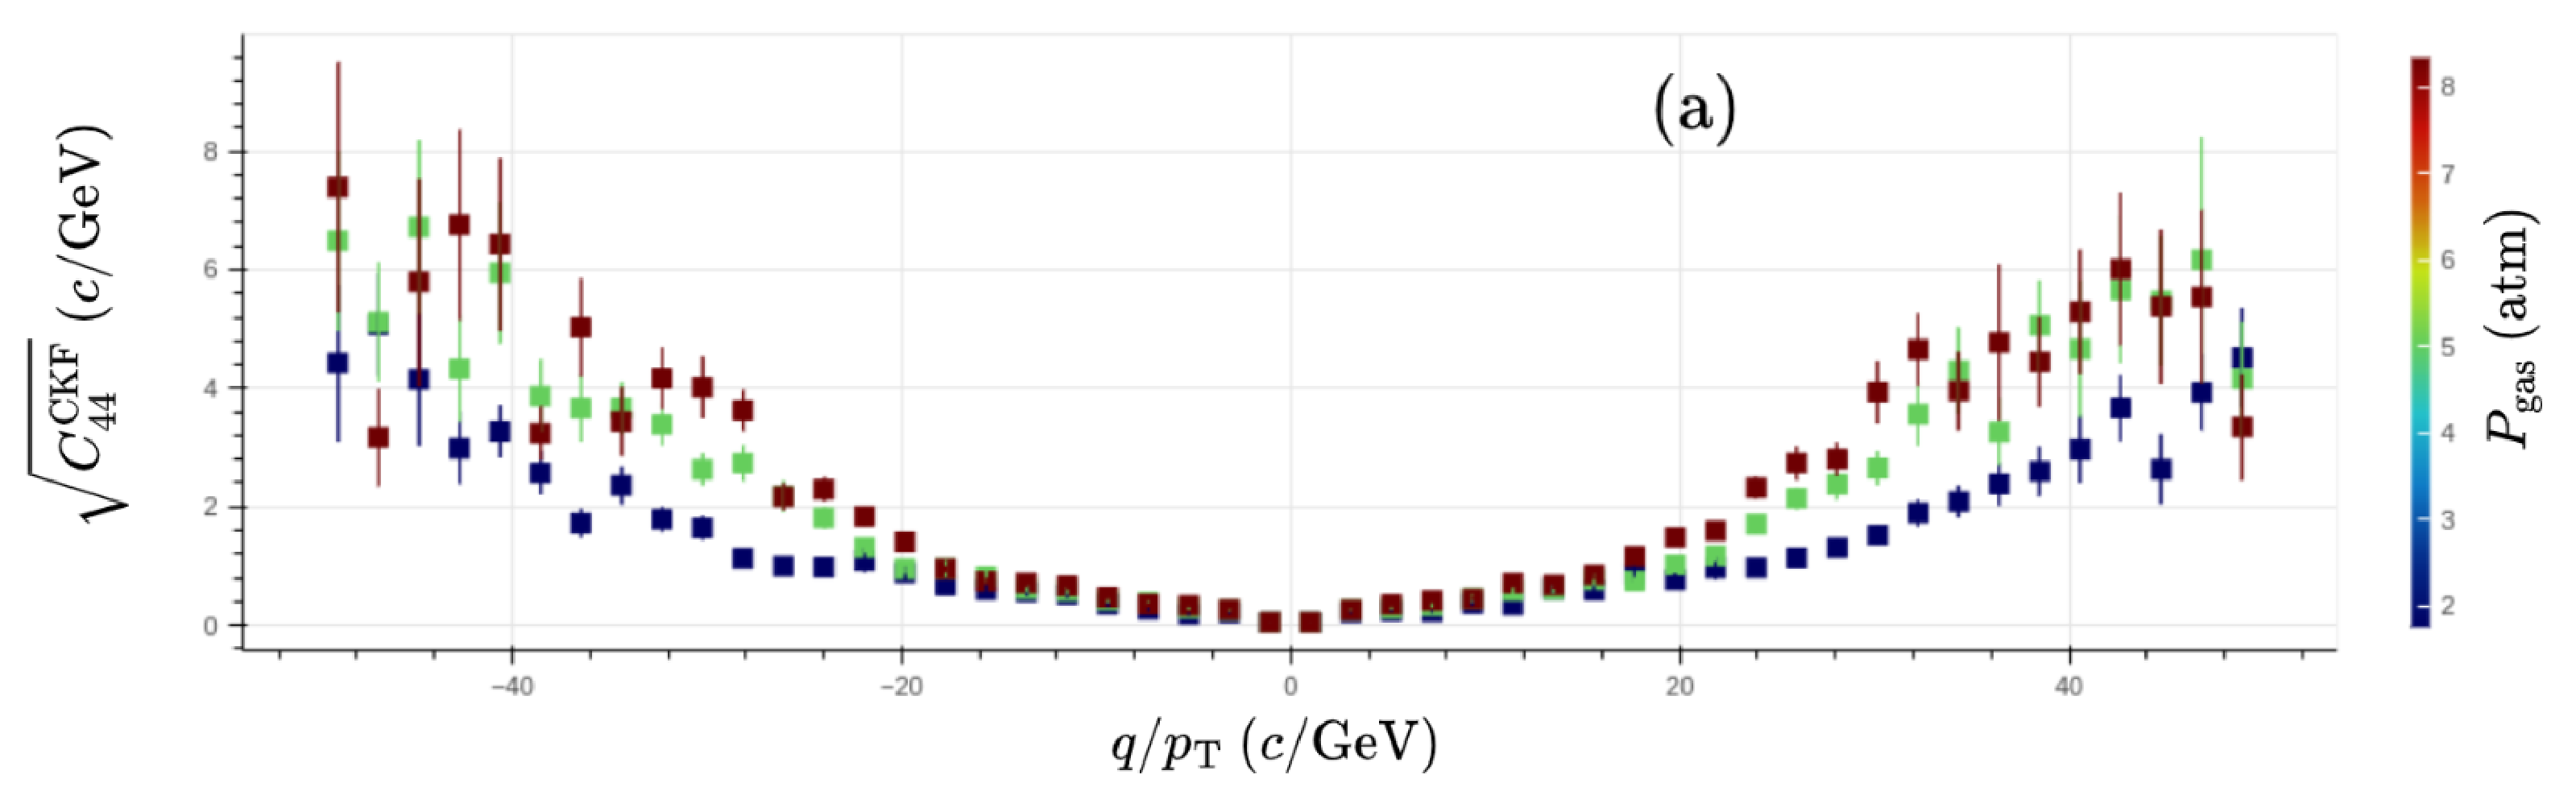
\includegraphics[width=\textwidth]{figures/ch5-KF_NDGAr/ToySample/ParScan/TotVSExpVSdens_noNorm_label.eps}
         \caption{}
         \label{fig:CheckAna_dens_noNorm}
     \end{subfigure}
     \begin{subfigure}[b]{0.99\textwidth}
         \centering
         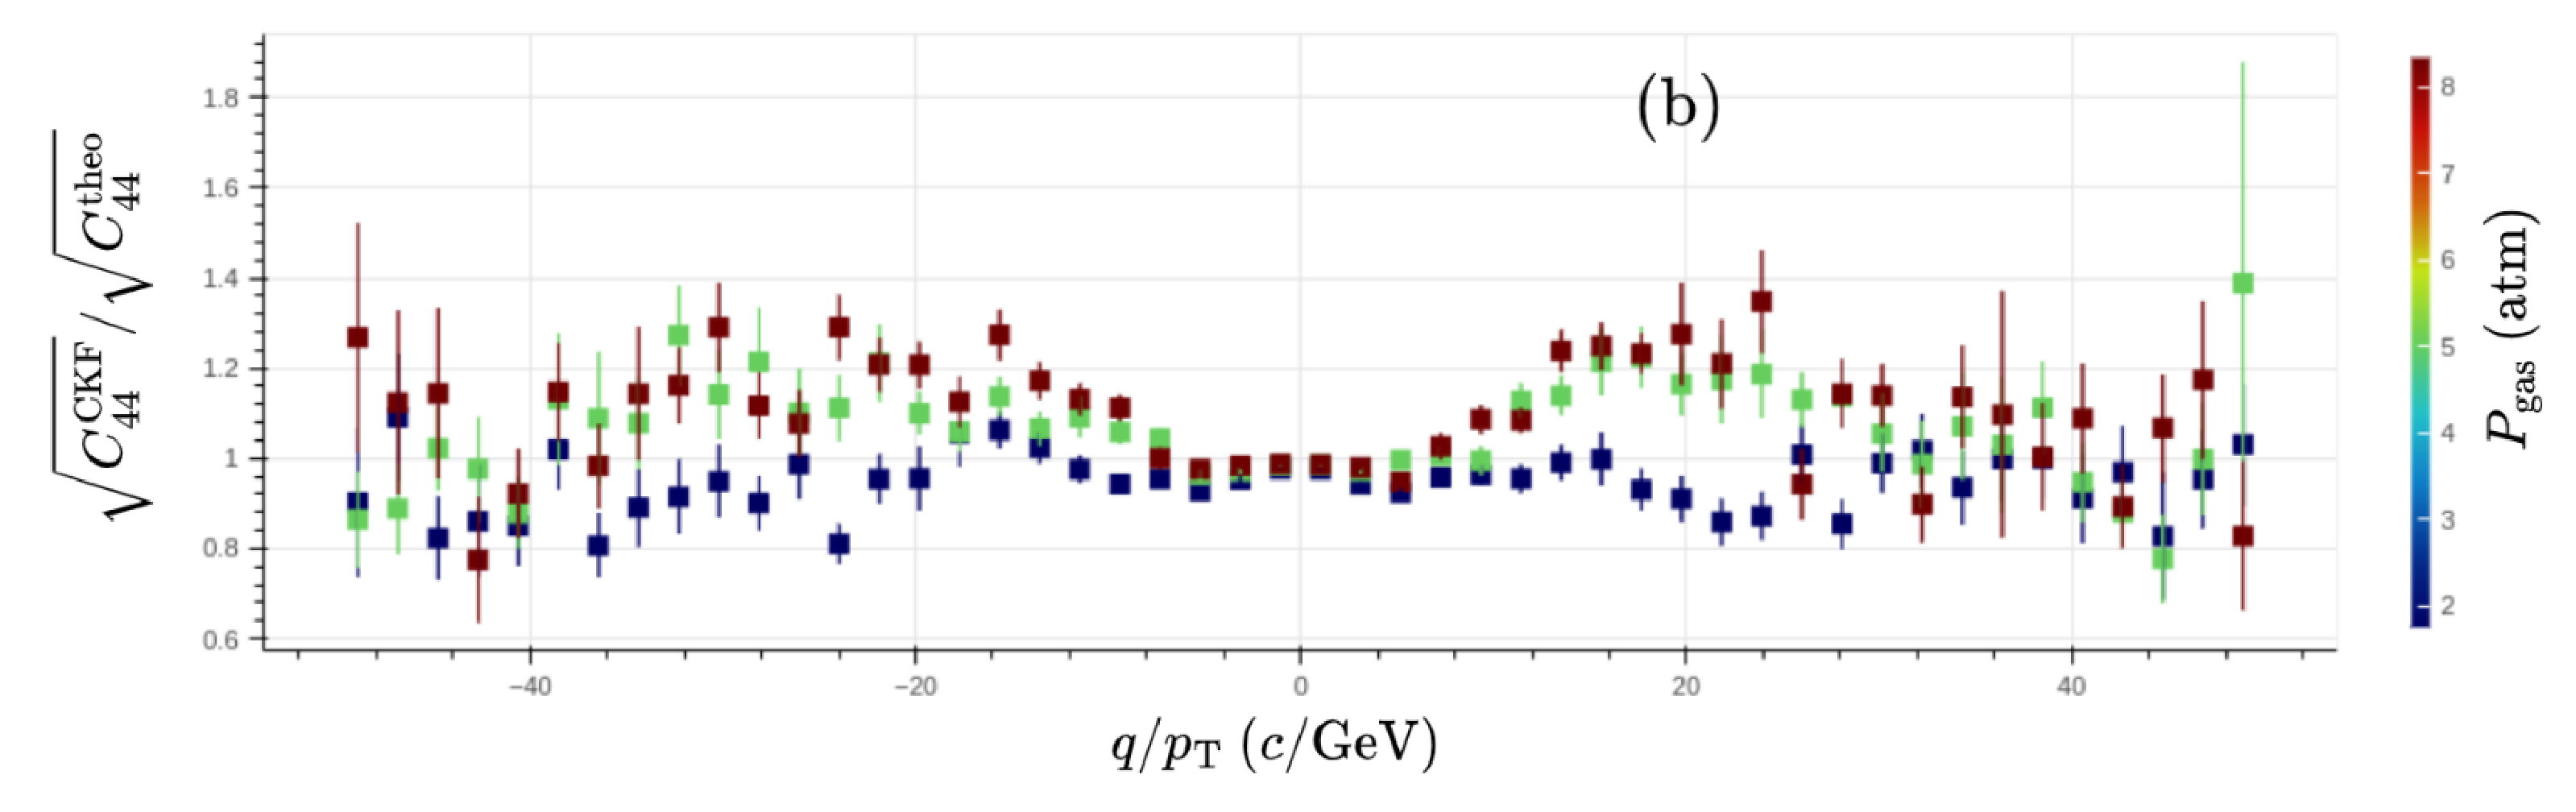
\includegraphics[width=\textwidth]{figures/ch5-KF_NDGAr/ToySample/ParScan/TotVSExpVSdens_label.eps}
         \caption{}
         \label{fig:CheckAna_dens_Norm}
     \end{subfigure}
        \caption[Similar plots to the ones presented in Fig.~\ref{fig:Check_Ana_pID}. The histograms in this case are color-coded according to the gas pressure $P_{\textrm{gas}}$.]{ Similar plots to the ones presented in Fig.~\ref{fig:Check_Ana_pID}. The histograms in this case are color-coded according to the gas pressure $P_{\textrm{gas}}$.}
        \label{fig:CheckAna_dens}
\end{figure}
\begin{figure}[!ht]
     \centering
     \begin{subfigure}[b]{0.99\textwidth}
         \centering
         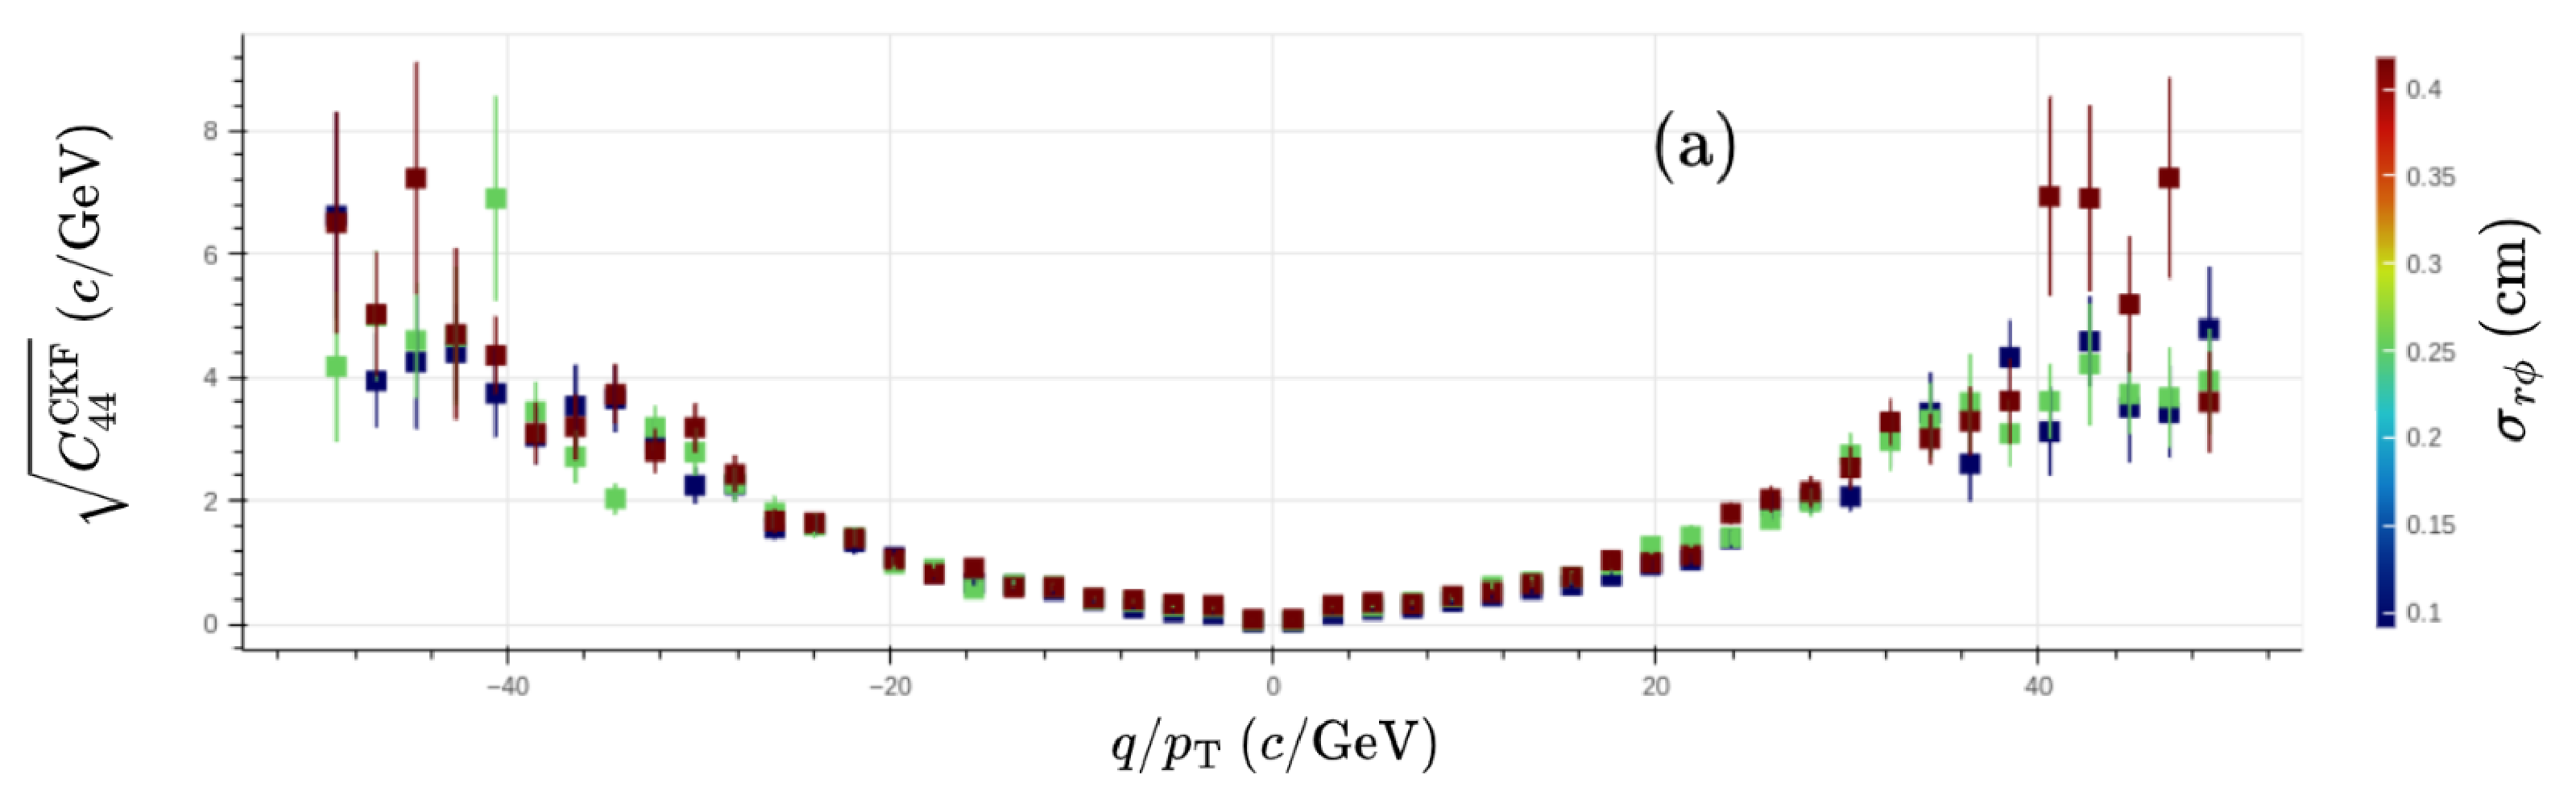
\includegraphics[width=\textwidth]{figures/ch5-KF_NDGAr/ToySample/ParScan/TotVSExpVSres_noNorm_label.eps}
         \caption{}
         \label{fig:CheckAna_res_noNorm}
     \end{subfigure}
     \begin{subfigure}[b]{0.99\textwidth}
         \centering
         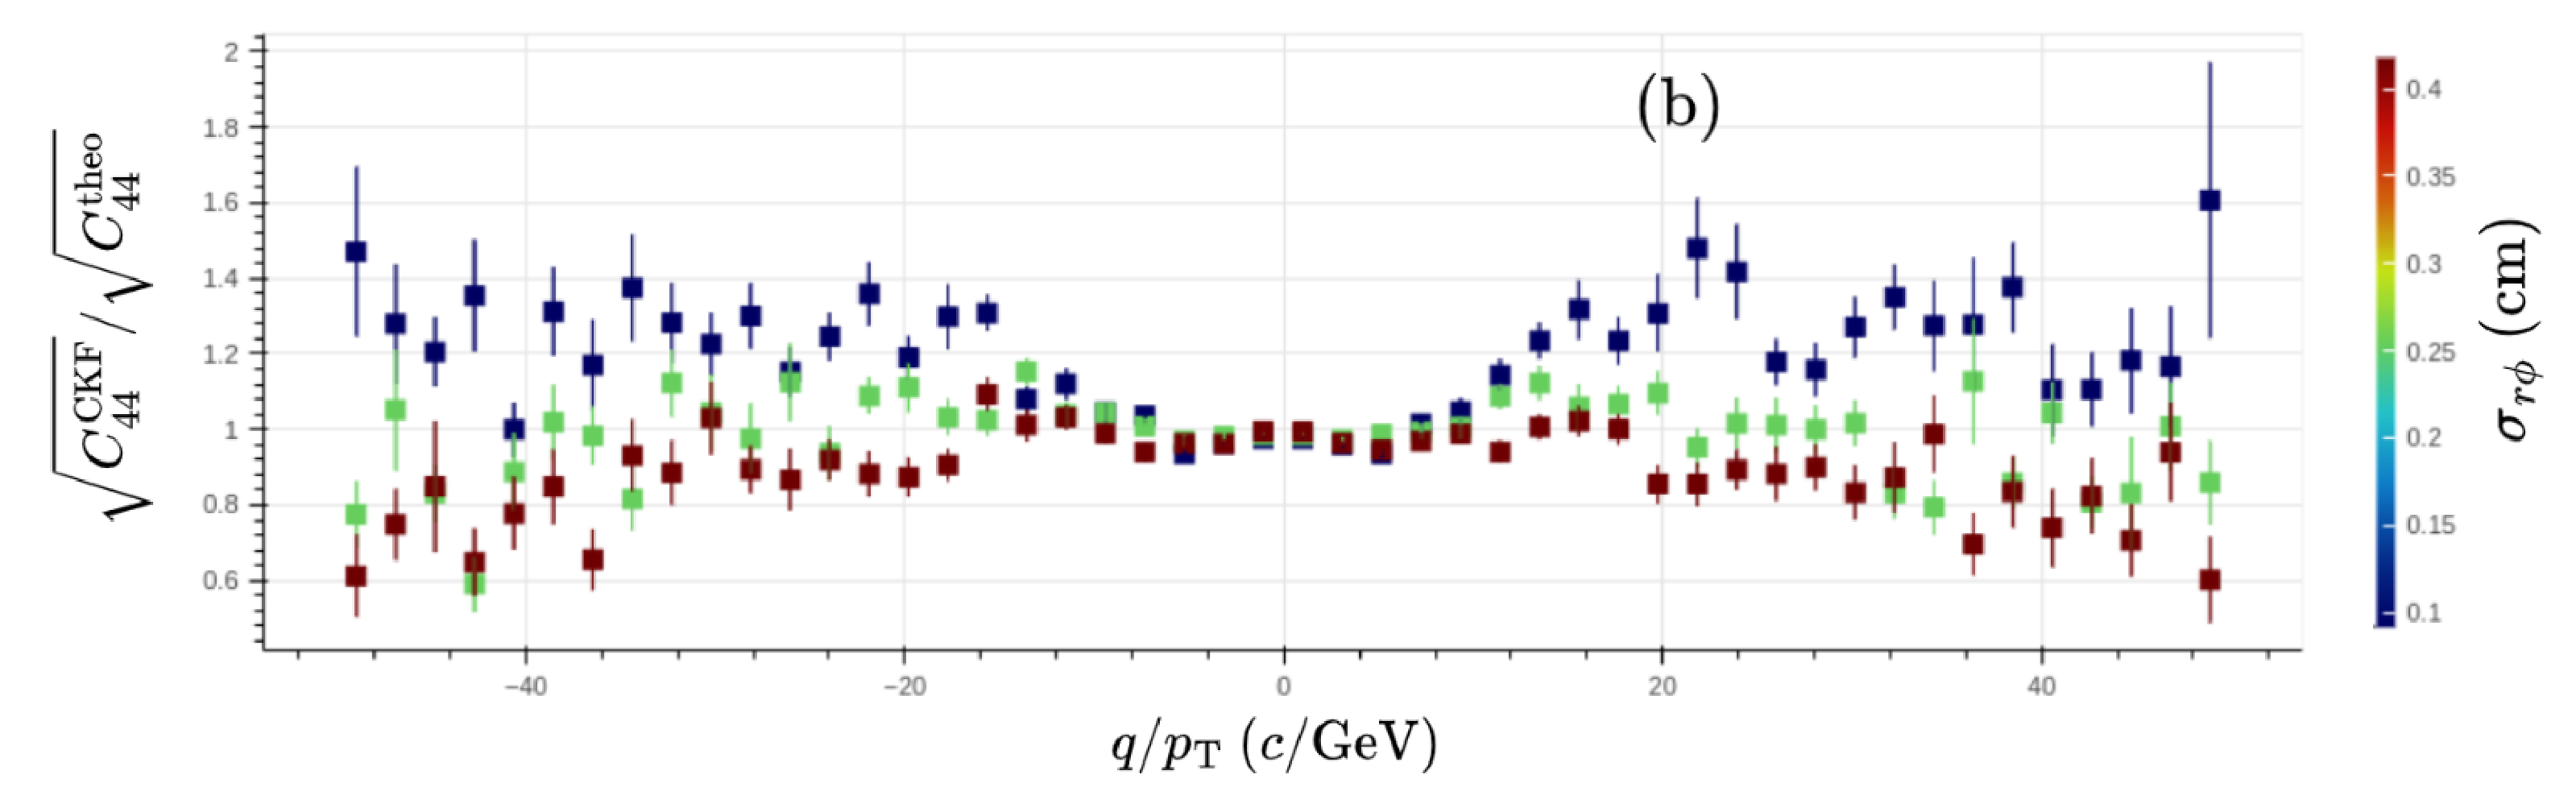
\includegraphics[width=\textwidth]{figures/ch5-KF_NDGAr/ToySample/ParScan/TotVSExpVSres_label.eps}
         \caption{}
         \label{fig:CheckAna_res_Norm}
     \end{subfigure}
        \caption[Similar plots to the ones presented in Fig.~\ref{fig:Check_Ana_pID}. The histograms in this case are color-coded according to the radial resolution $\sigma_{r\phi}$.]{Similar plots to the ones presented in Fig.~\ref{fig:Check_Ana_pID}. The histograms in this case are color-coded according to the radial resolution $\sigma_{r\phi}$.}
        \label{fig:Check_Ana_res}
\end{figure} 

In Fig.~\ref{fig:Check_Ana_pID},the histograms are color-scaled based on particle type, denoted as $t_\textrm{ID}$. Conversely, in Figs.~\ref{fig:CheckAna_dens} and ~\ref{fig:Check_Ana_res}, the color scaling corresponds to gas pressure, $P_{\textrm{gas}}$, and point resolution $\sigma_{r\phi}=\sigma_z$ respectively. The \texttt{CKF} results show overall good agreement with the theoretical expectation, with ratios $\sim 1$ for momenta down to 20 MeV/$c$ within statistical uncertainties.

The PS sample was further used to test the improvement in $q/p_{\text{T}}$ resolution brought by the introduction of the \enquote{mirror rotation} technique in the \texttt{CKF}, compared to \texttt{BKF}. The fraction of the total tracks for which the mirroring technique was used $\epsilon_\textrm{Mirror}$ is shown in Fig.~\ref{fig:MirrorRatio} as a function of initial true $p_\textrm{T}$ and $P_\textrm{gas}$. We show the fraction for the primaries in the first row and for the secondaries in the second. The particle types are divided in order of mass between electrons in Figs. \ref{fig:MirrorRatiop_Prim_e} and \ref{fig:MirrorRatiop_Sec_e}, muons and pions in Figs. \ref{fig:MirrorRatio_Prim_mu} and \ref{fig:MirrorRatio_Sec_mu}, kaons and protons in Figs. \ref{fig:MirrorRation_Prim_k} and \ref{fig:MirrorRation_Sec_k}. We can see from the upper row plots and the low $p_\textrm{T}$ component of the lower row plots that the likelihood of the particles producing looping trajectory drops significantly with mass, due to the higher $\textrm{d}E/\textrm{d}x$. At low momenta the pressure of the gas also becomes important. This is especially true for the higher mass particles such as protons and kaons, which at higher $P_\textrm{gas}$ are stopped in the detector before producing any looping trajectory (see Fig. \ref{fig:MirrorRation_Prim_k}). From Figs. \ref{fig:MirrorRatiop_Sec_e}, \ref{fig:MirrorRatio_Prim_mu} and \ref{fig:MirrorRation_Sec_k} it can also be shown that the only primary particle that necessitate the use of the mirroring operation are those that produce a looping trajectory in the detector, which is only possible at low initial transverse momenta $p_\textrm{T}<0.3 \ \textrm{GeV}/c$ (see Eq.~\ref{eq:curvatureconv}).  Secondary particle trajectories, on the other hand, can cover more than a semi-plane even if they don't belong to loopers and can thus be produced at any momenta, as shown in Figs. \ref{fig:MirrorRatiop_Sec_e}, \ref{fig:MirrorRatio_Prim_mu} and \ref{fig:MirrorRation_Sec_k}. At low transverse momenta, $\epsilon_\textrm{Mirror}$ is still significantly higher for secondaries. 

The reconstruction efficiency $\epsilon$, defined as the fraction of the correctly simulated tracks for which the algorithm is fully propagated, was tested for \texttt{CKF} and \texttt{BKF}. It is shown as a function of the initial true $p_\textrm{T}$ and the $N$ of the total track in the first and second column of Fig \ref{fig:PS_Eff} respectively. In Figs. \ref{fig:PS_Eff_CKF_Mirror} and \ref{fig:PS_Eff_BKF_Mirror} only the tracks for which the mirroring technique is used are shown, while the other tracks are shown Figs. \ref{fig:PS_Eff_CKF_NoMirror} and \ref{fig:PS_Eff_BKF_NoMirror}. For the ``non-mirrored'' tracks the efficiency is essentially identical between the \texttt{BKF} and \texttt{CKF} algorithm and it is shown to be very close to 1 except for very low $p_\textrm{T}$ and $N$, for which other approaches  than a Kalman Filter would most likely be used~\cite{RevModPhys.82.1419}. On the other hand $\epsilon$ is significantly improved by the \texttt{CKF} for low $N$ ``mirrored'' tracks, in some cases going from an efficiency of $\sim0.5$ to $\epsilon>0.9$. This is a direct consequence of the increased number of points becoming available through the use of the mirroring technique.   

\begin{figure}[!ht]
     \centering
     \begin{subfigure}[b]{0.32\textwidth}
         \centering
         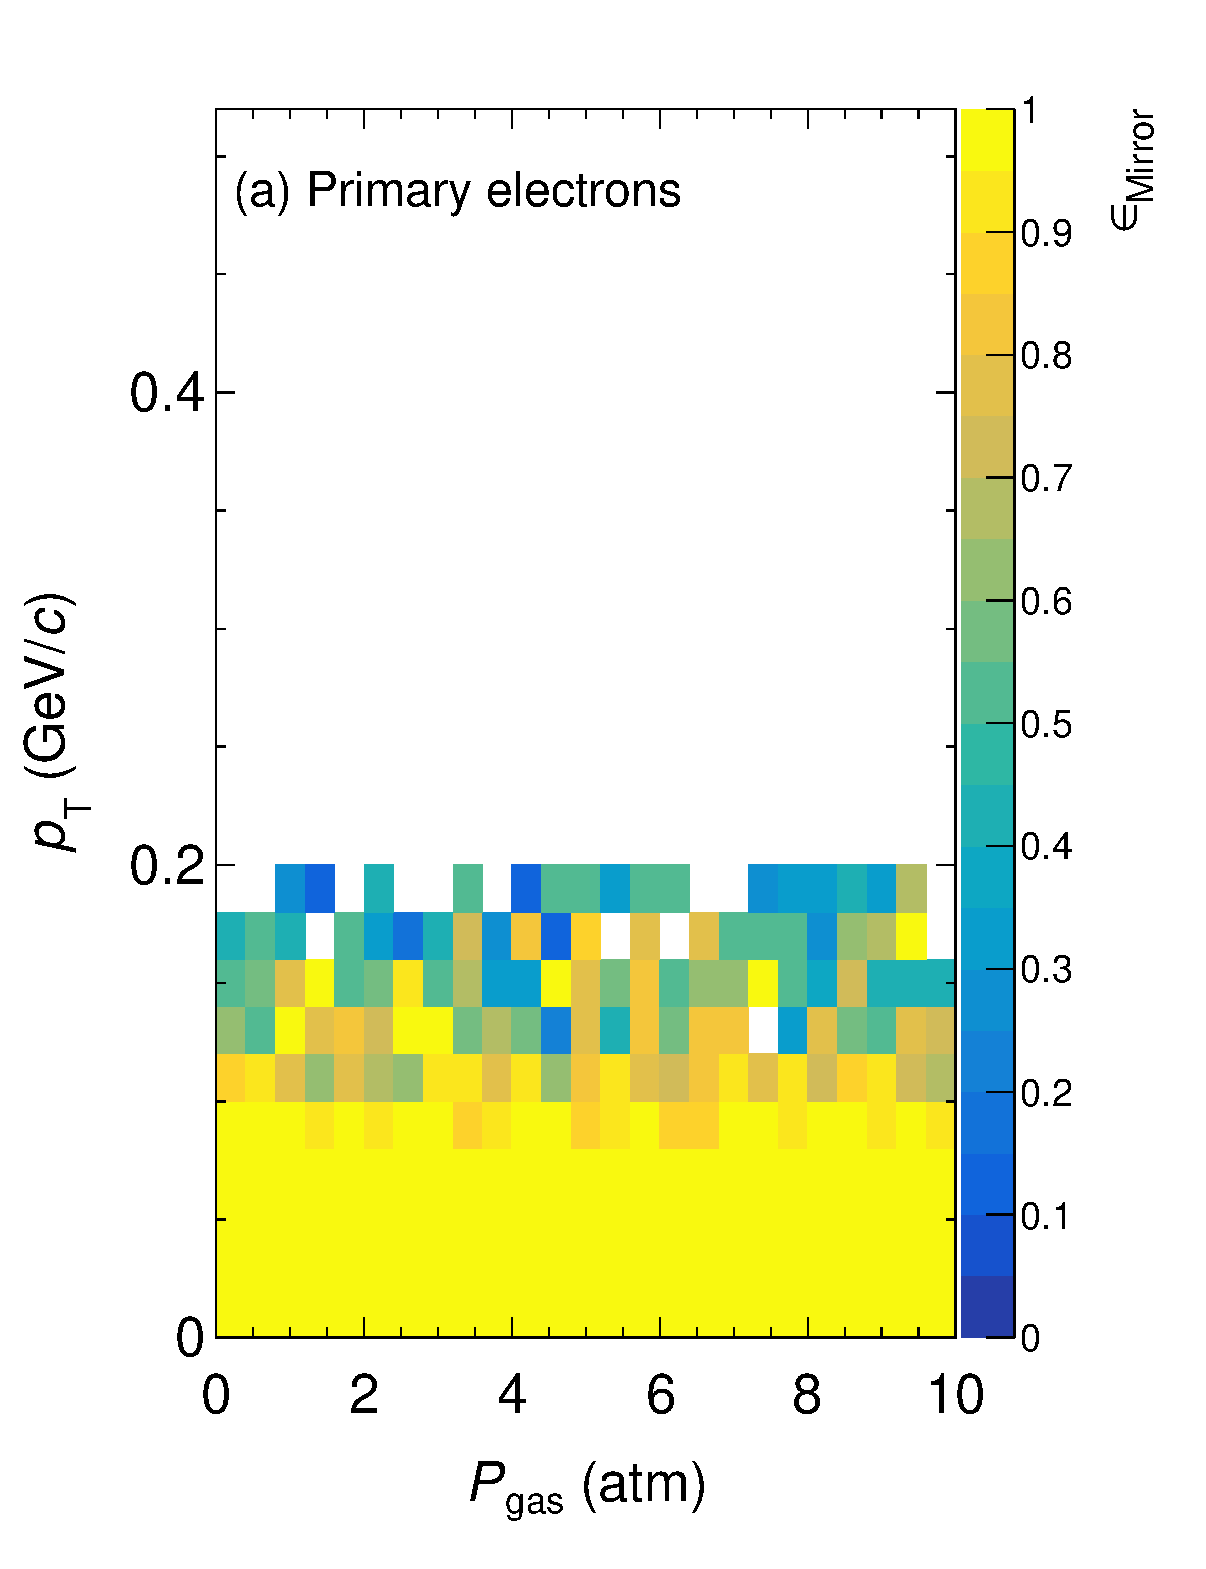
\includegraphics[width=\textwidth]{figures/ch5-KF_NDGAr/ToySample/ParScan/testTPCMirrorMirrorRatioVSpTVSdens_e.eps}
         \caption{}
         \label{fig:MirrorRatiop_Prim_e}
     \end{subfigure}
     \begin{subfigure}[b]{0.32\textwidth}
         \centering
         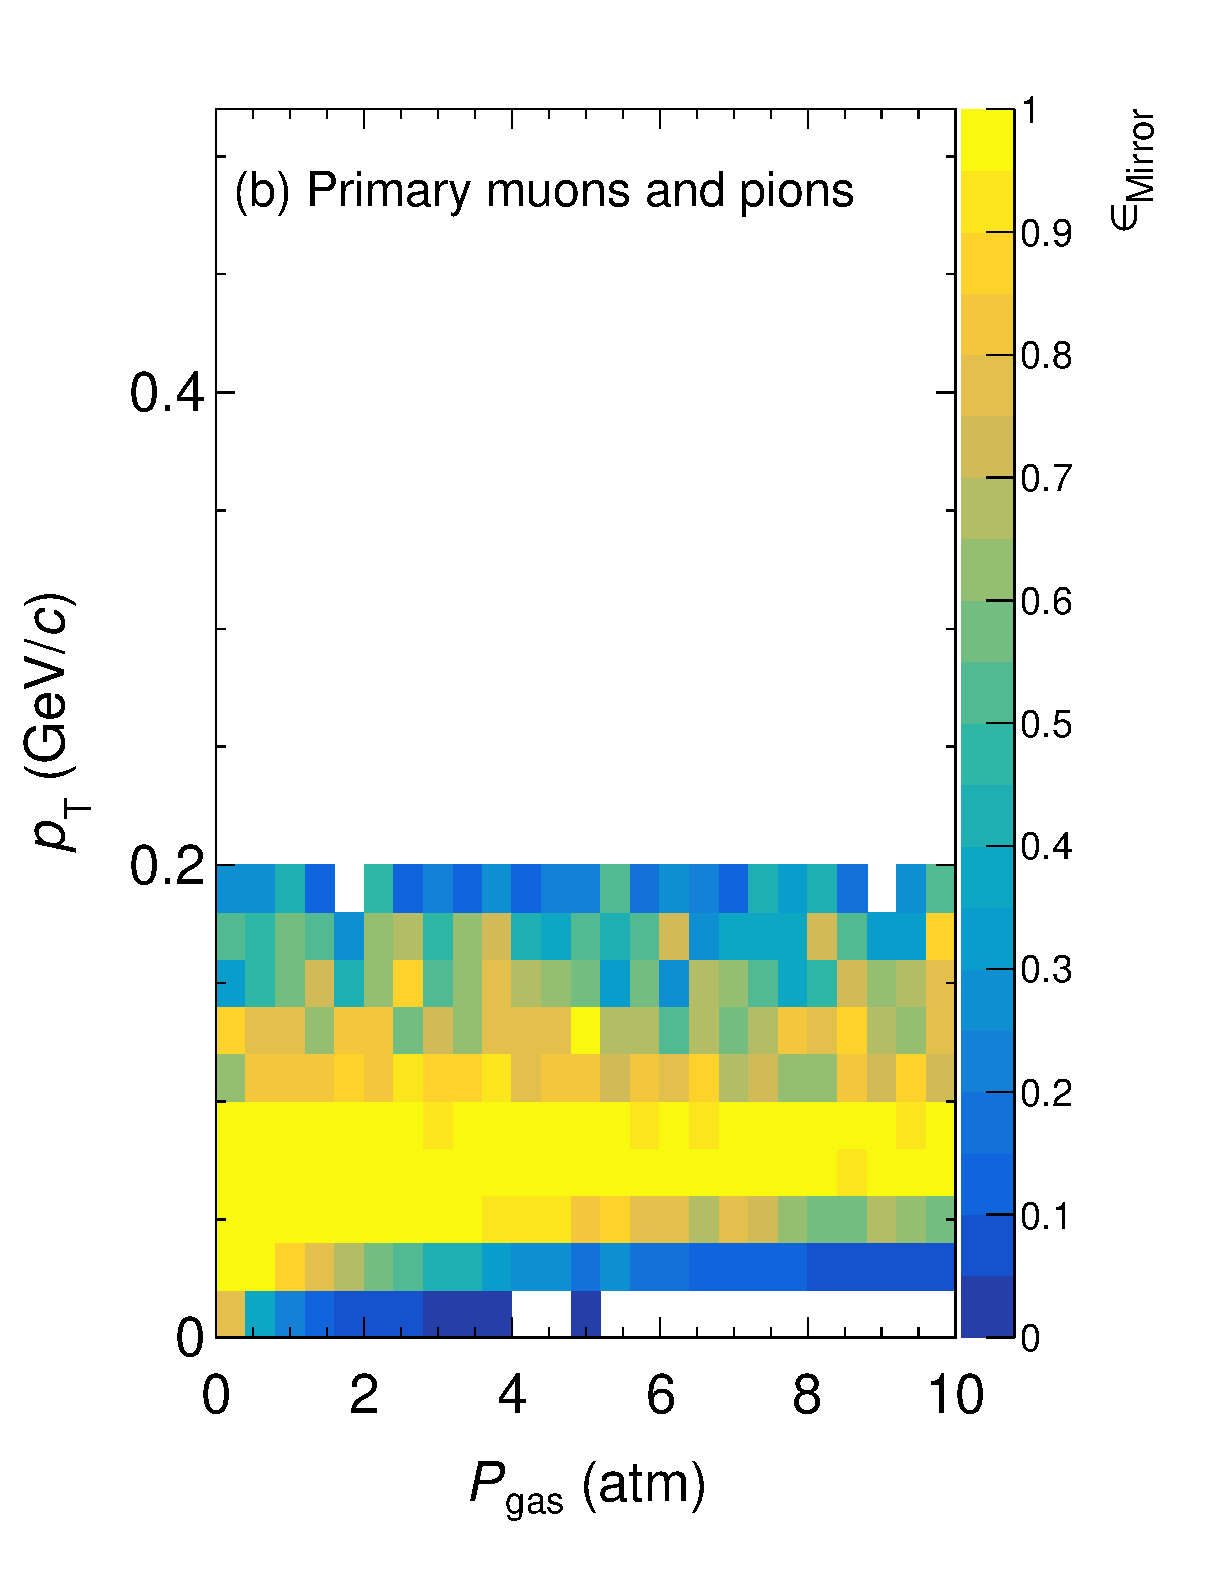
\includegraphics[width=\textwidth]{figures/ch5-KF_NDGAr/ToySample/ParScan/testTPCMirrorMirrorRatioVSpTVSdens_mupi.eps}
         \caption{}
         \label{fig:MirrorRatio_Prim_mu}
     \end{subfigure}
          \begin{subfigure}[b]{0.32\textwidth}
         \centering
         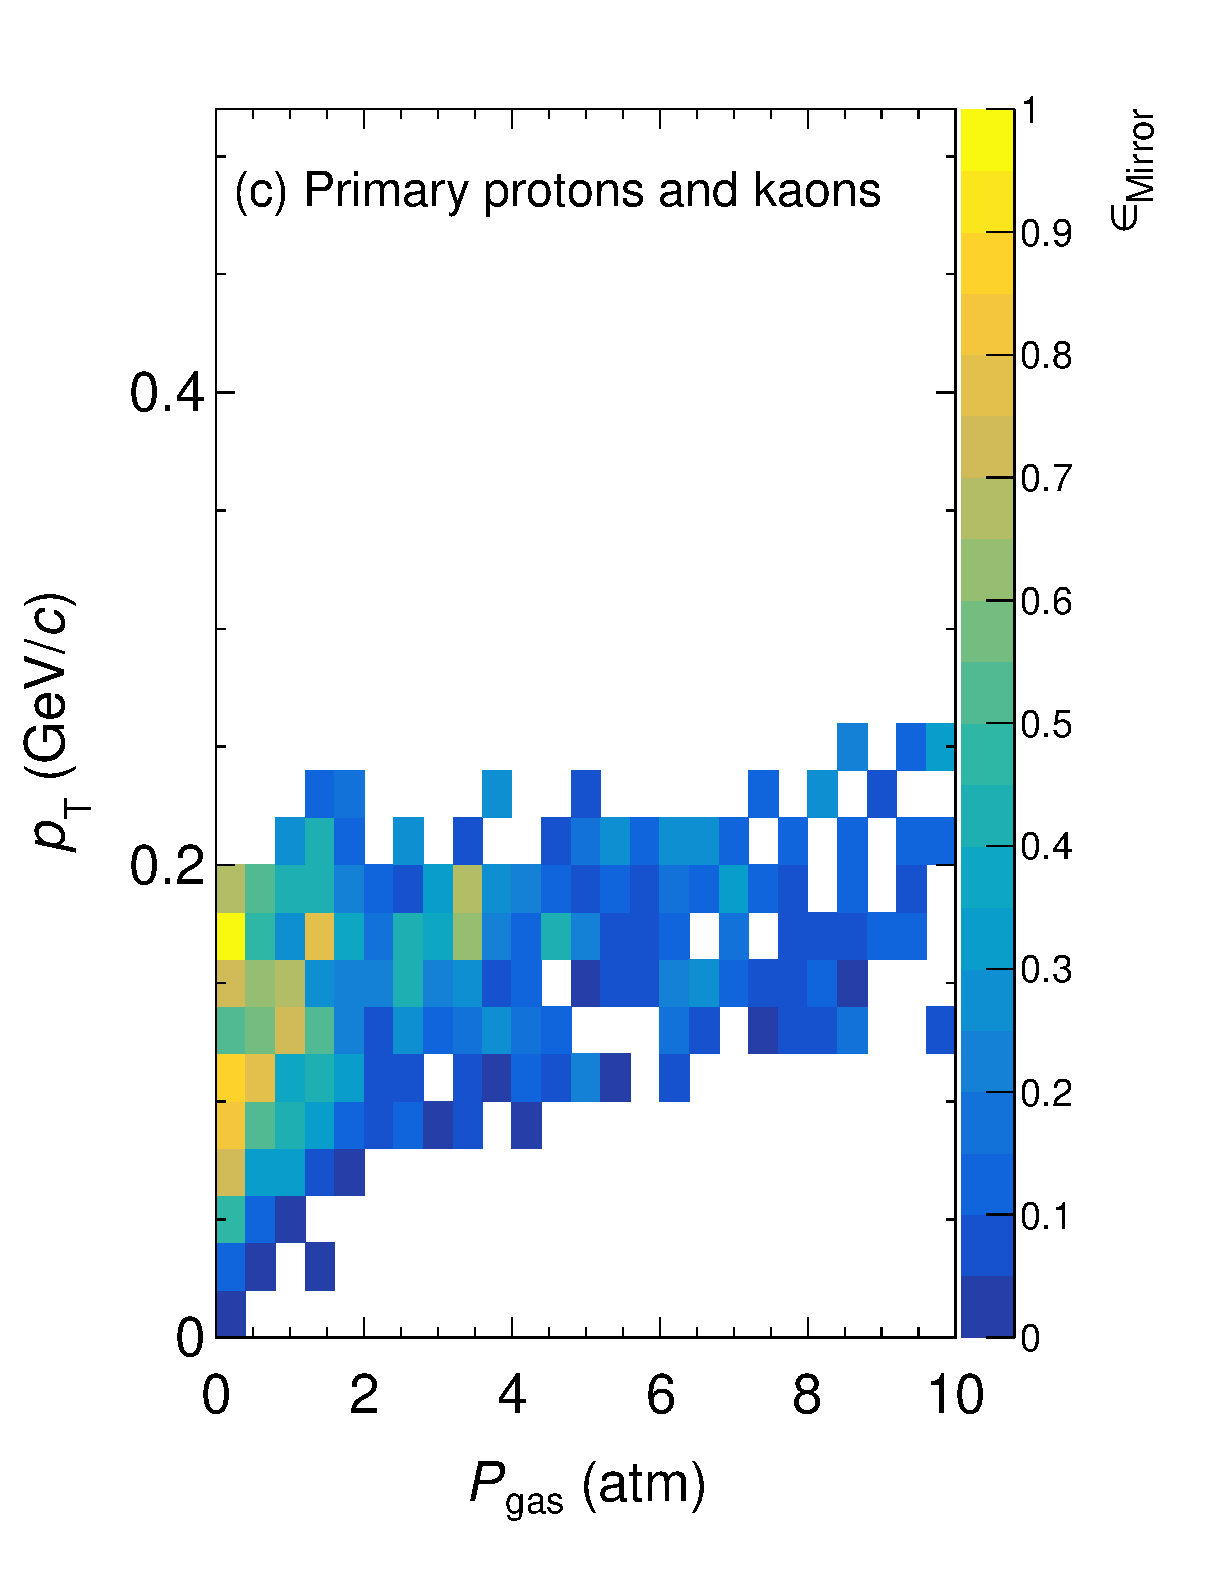
\includegraphics[width=\textwidth]{figures/ch5-KF_NDGAr/ToySample/ParScan/testTPCMirrorMirrorRatioVSpTVSdens_kp.eps}
         \caption{}
         \label{fig:MirrorRation_Prim_k}
     \end{subfigure}
     \begin{subfigure}[b]{0.32\textwidth}
         \centering
         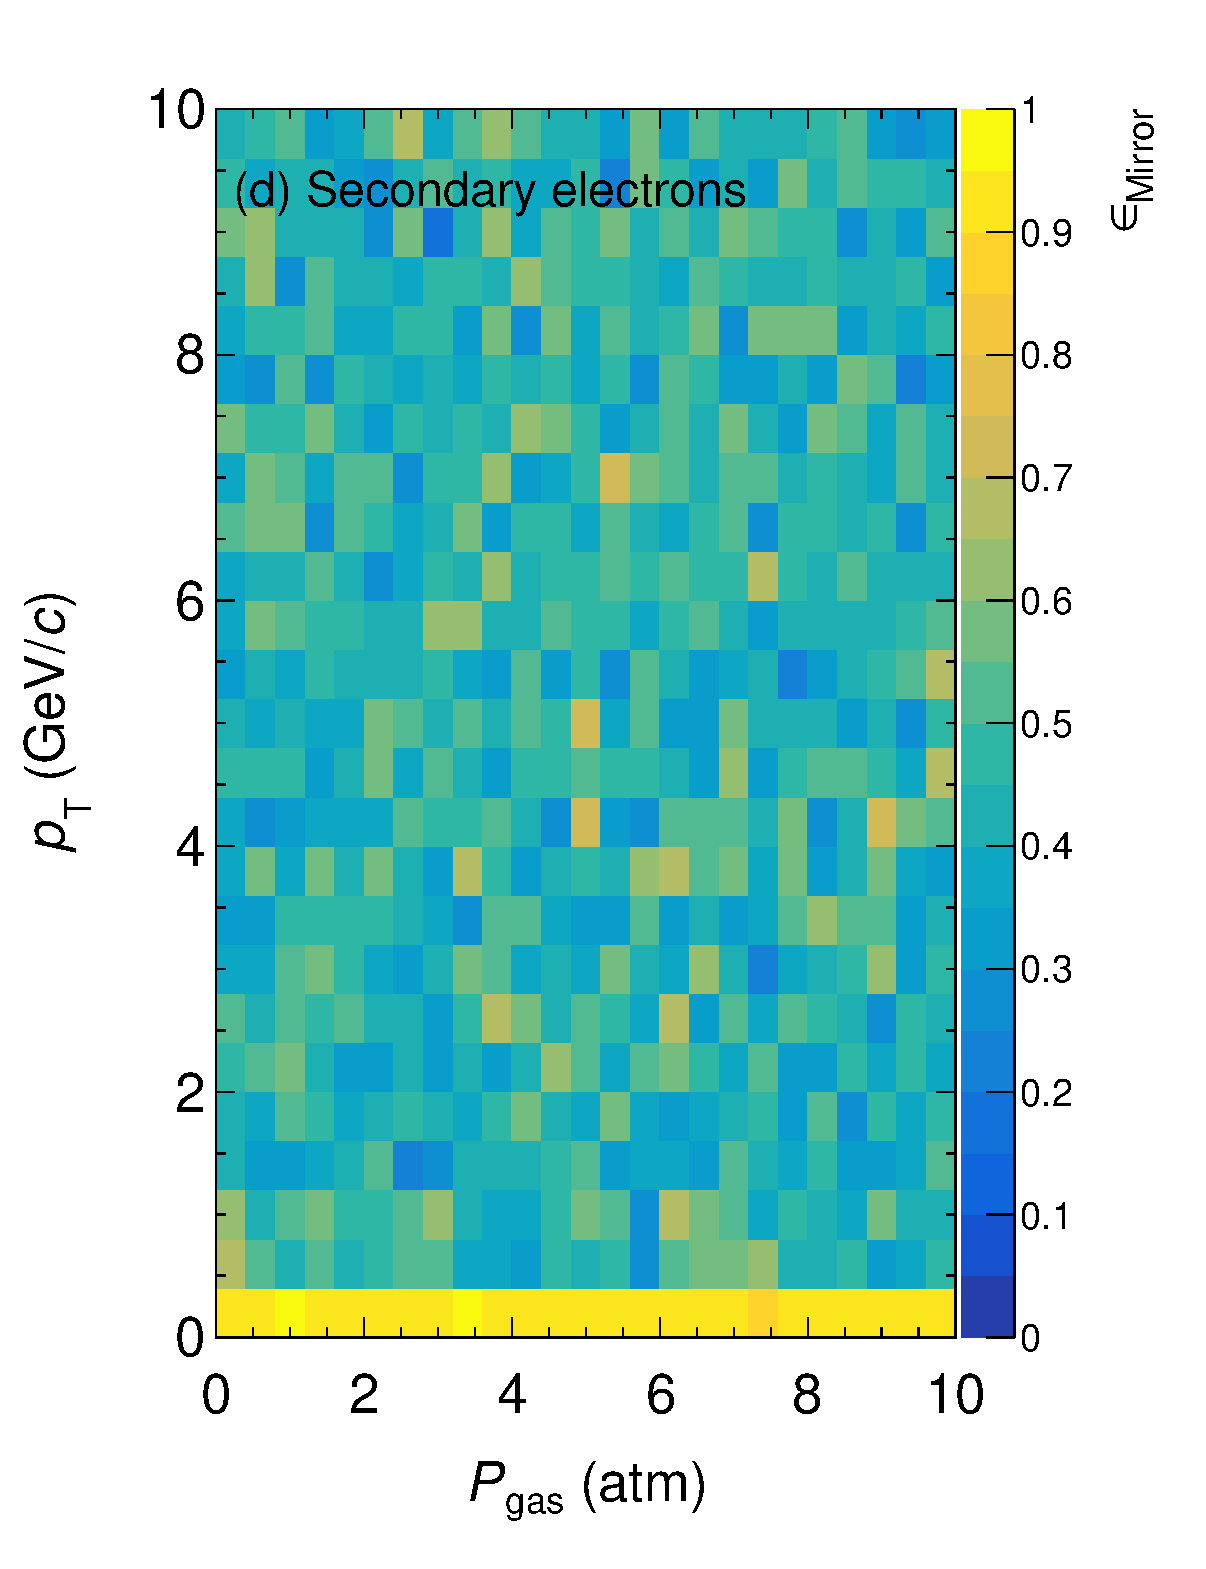
\includegraphics[width=\textwidth]{figures/ch5-KF_NDGAr/ToySample/ParScan/testTPCMirrorMirrorRatioVSpTVSdens_sec_e.eps}
         \caption{}
         \label{fig:MirrorRatiop_Sec_e}
     \end{subfigure}
     \begin{subfigure}[b]{0.32\textwidth}
         \centering
         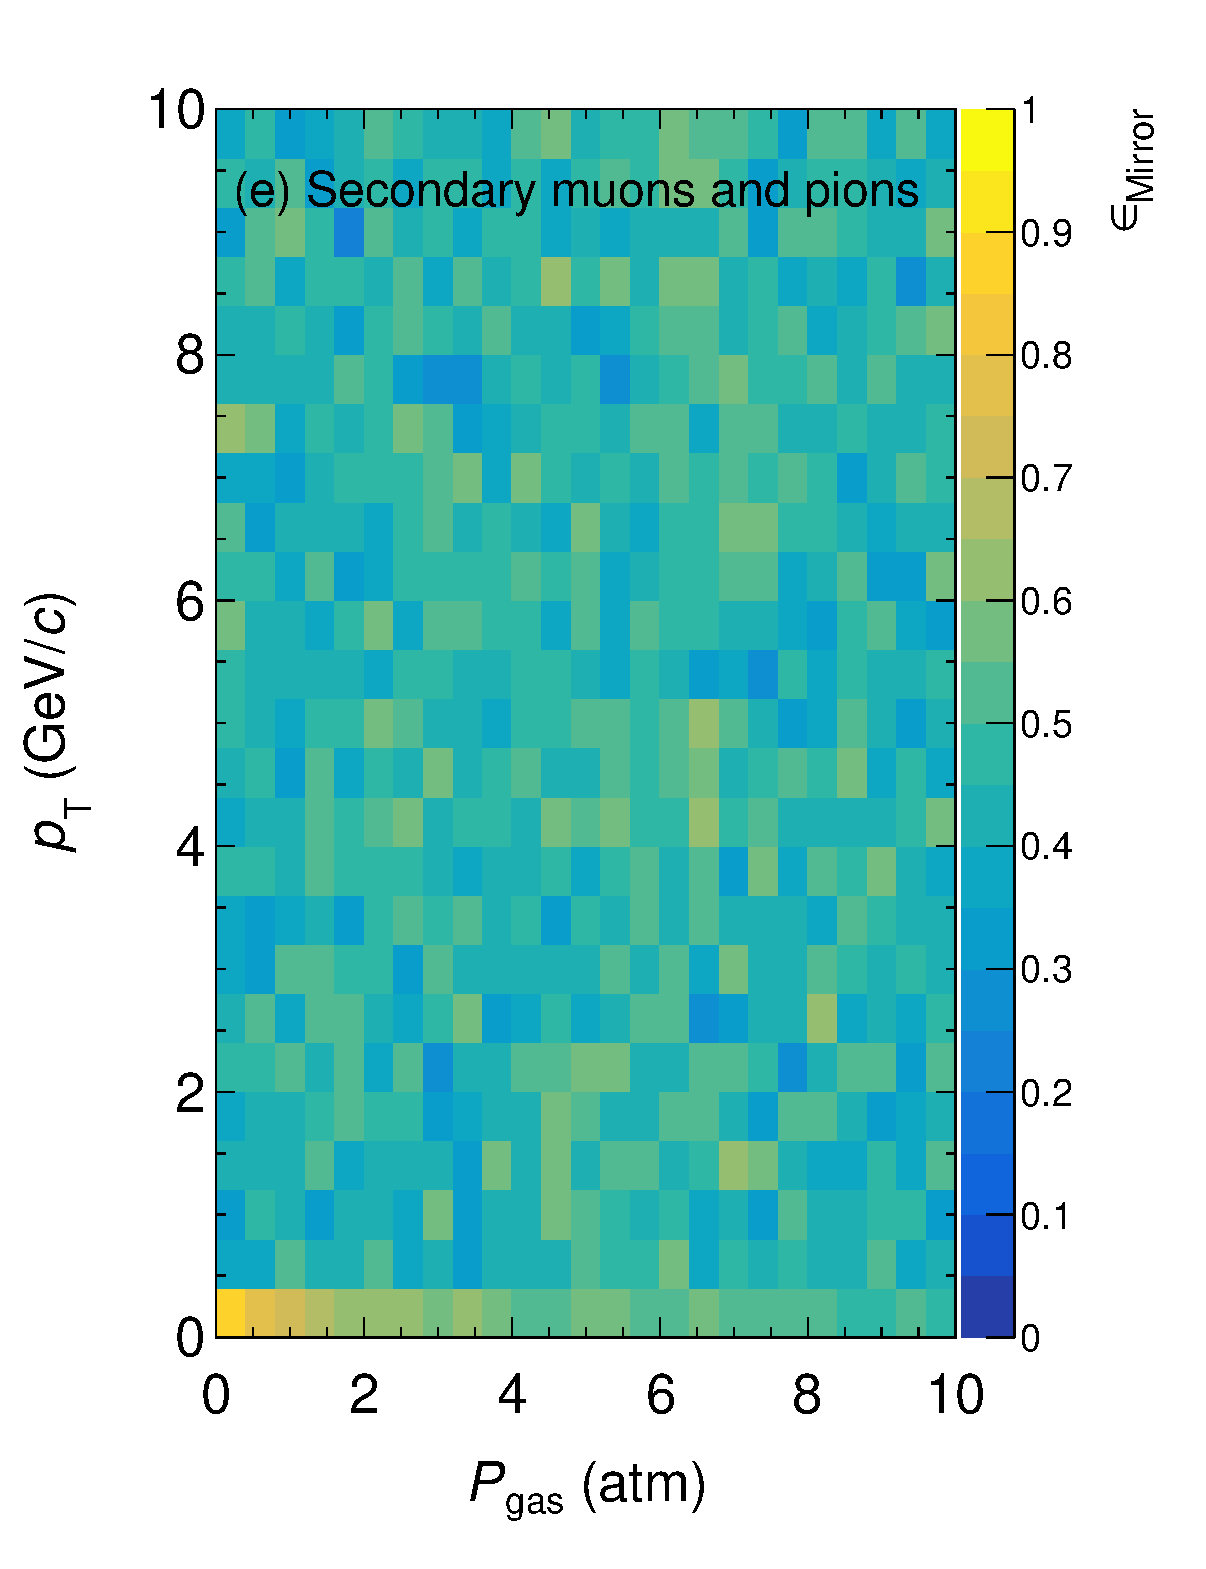
\includegraphics[width=\textwidth]{figures/ch5-KF_NDGAr/ToySample/ParScan/testTPCMirrorMirrorRatioVSpTVSdens_sec_mupi.eps}
         \caption{}
         \label{fig:MirrorRatio_Sec_mu}
     \end{subfigure}
          \begin{subfigure}[b]{0.32\textwidth}
         \centering
         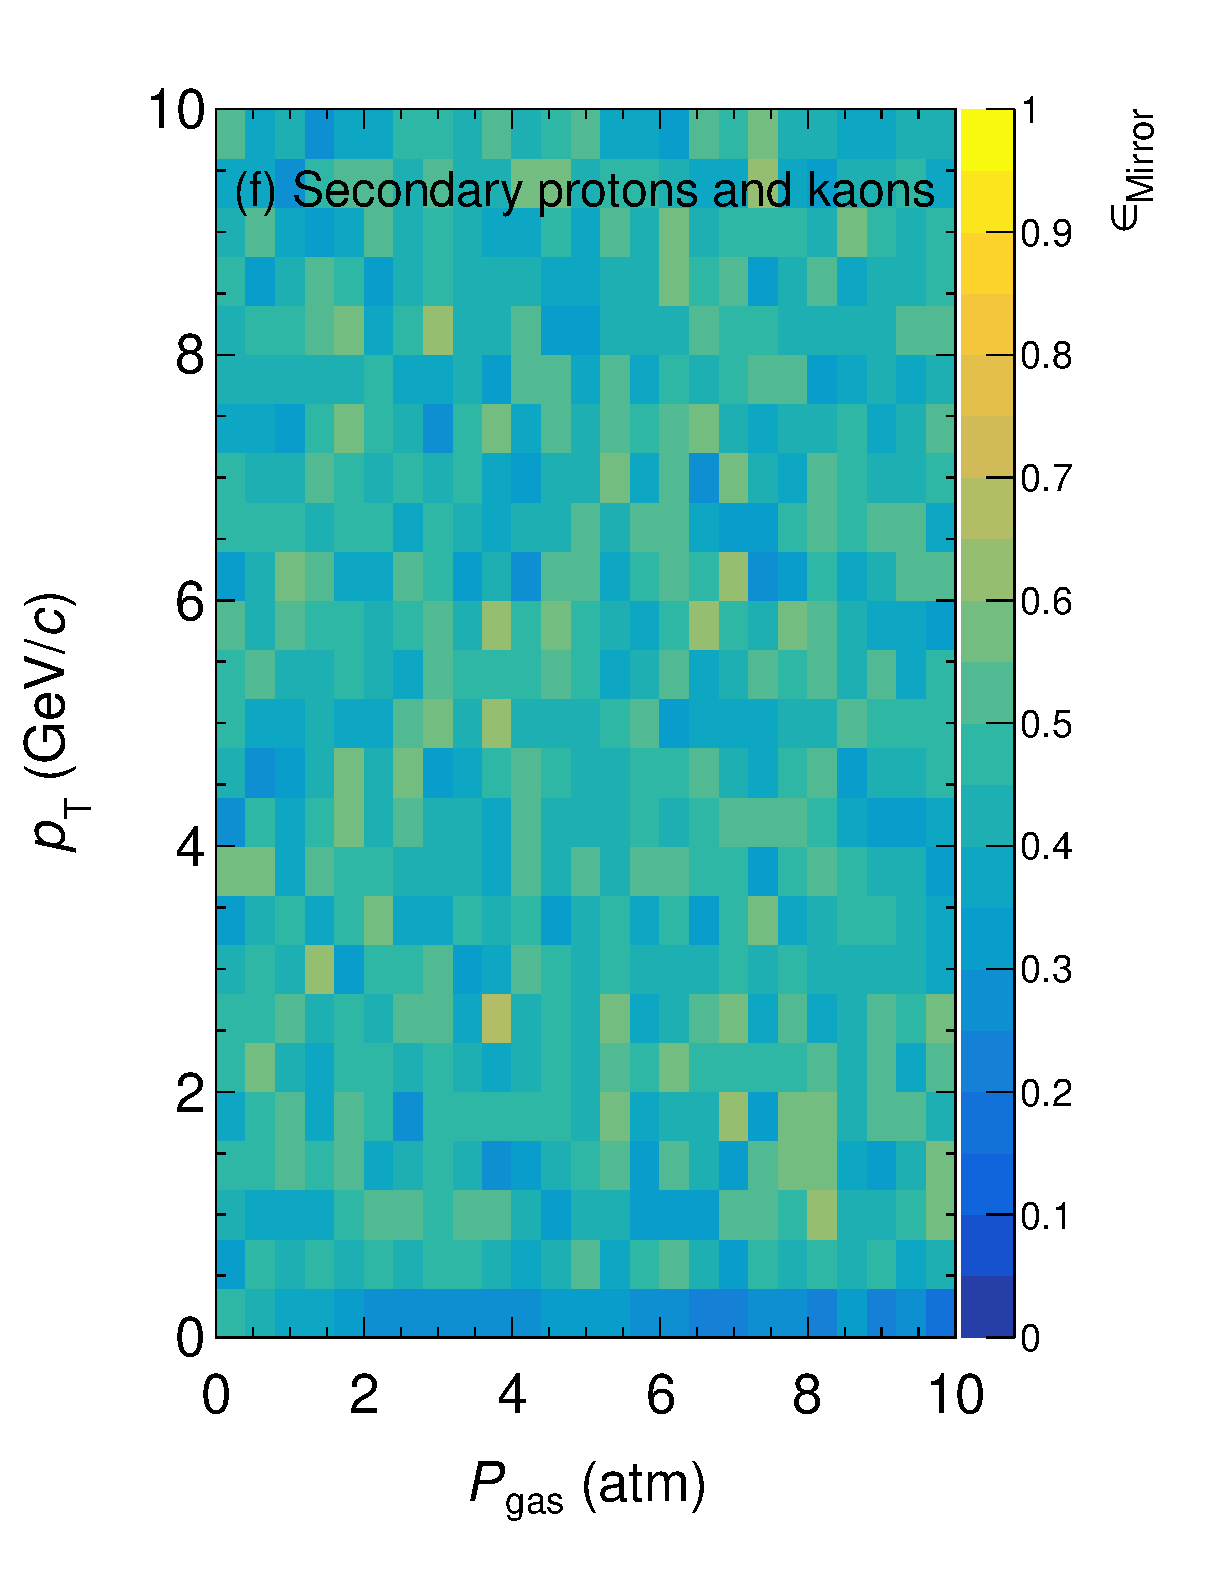
\includegraphics[width=\textwidth]{figures/ch5-KF_NDGAr/ToySample/ParScan/testTPCMirrorMirrorRatioVSpTVSdens_sec_kp.eps}
         \caption{}
         \label{fig:MirrorRation_Sec_k}
     \end{subfigure}
        \caption[Portion of tracks in the PS sample for which the mirror rotation was applied $\epsilon_\textrm{Mirror}$.]{ Portion of tracks in the PS sample for which the mirror rotation was applied, $\epsilon_\textrm{Mirror}$, as a function of the gas pressure $P_\textrm{gas}$ and the initial true transverse momentum $p_\textrm{T}$ of the particle. The primaries are shown in the upper row, while the secondaries are shown in the lower row. The particle types are separated based on their mass: (a) and (d) contain only electrons, (b) and (e) muons and pions, (c) and (f) kaons and protons.} \label{fig:MirrorRatio}
\end{figure}

\begin{figure}[!ht]
     \centering
     \begin{subfigure}[b]{0.48\textwidth}
         \centering
         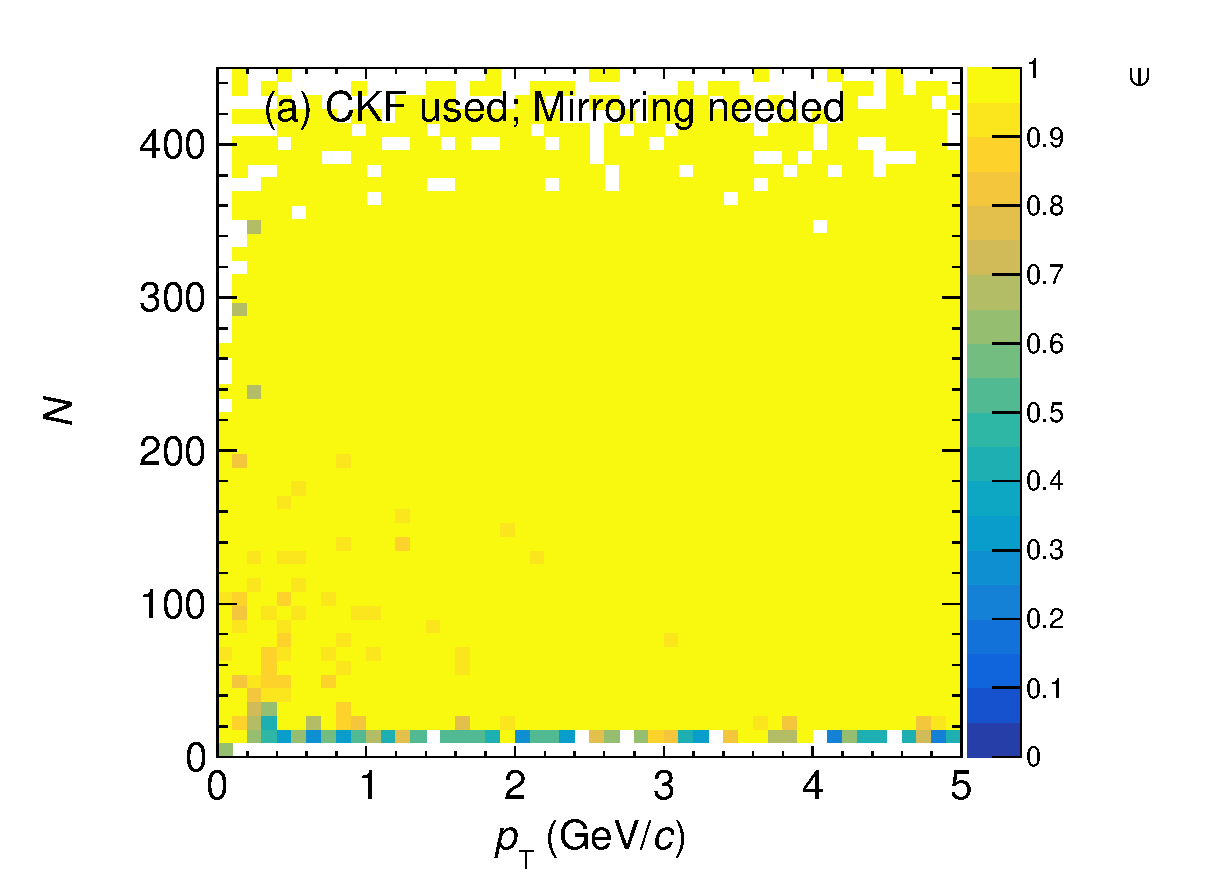
\includegraphics[width=\textwidth]{figures/ch5-KF_NDGAr/ToySample/ParScan/testNDGArMirrorEfficiencyVSNPointsVSpT_Mirror.eps}
         \caption{}
         \label{fig:PS_Eff_CKF_Mirror}
     \end{subfigure}
     \begin{subfigure}[b]{0.48\textwidth}
         \centering
         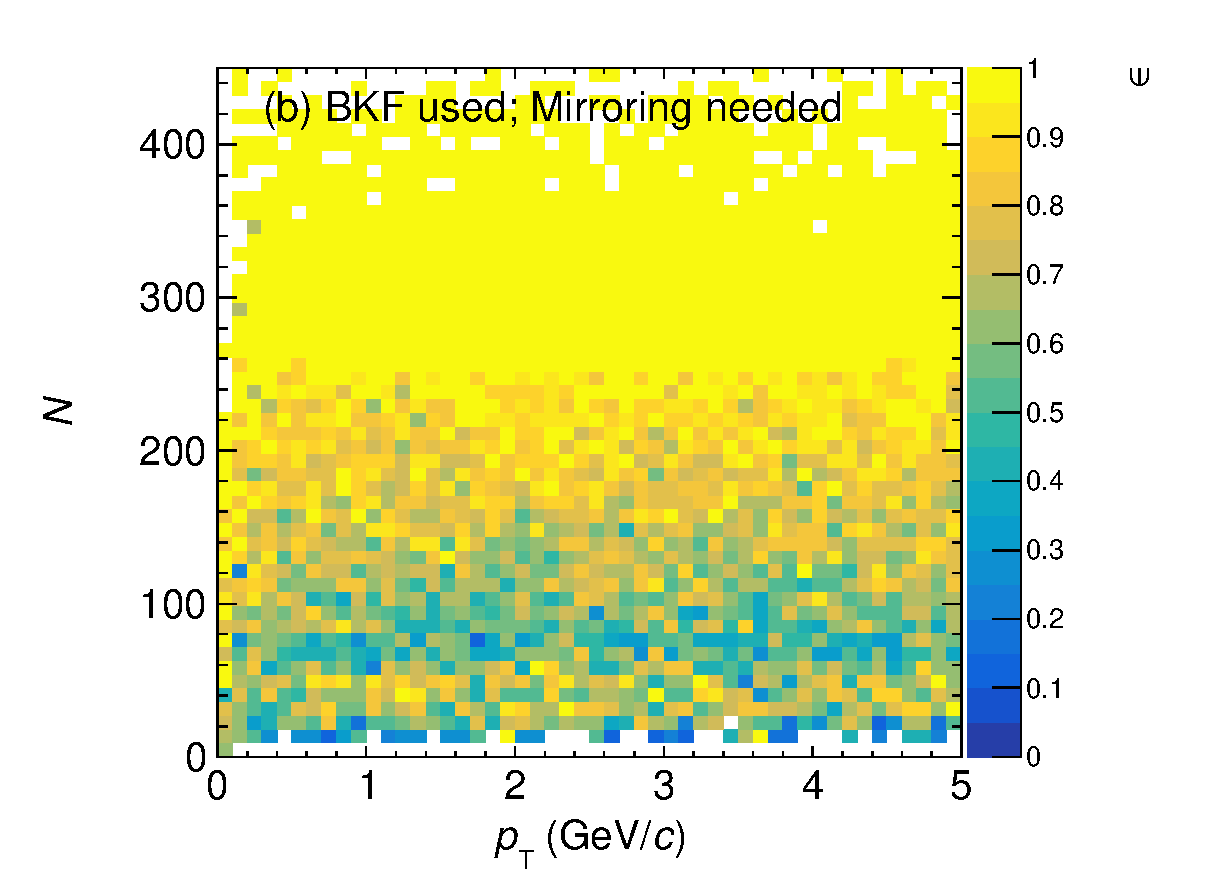
\includegraphics[width=\textwidth]{figures/ch5-KF_NDGAr/ToySample/ParScan/testNDGArMirrorEfficiencyVSNPointsVSpT_BKF_Mirror.eps}
         \caption{}
         \label{fig:PS_Eff_BKF_Mirror}
     \end{subfigure}
          \begin{subfigure}[b]{0.48\textwidth}
         \centering
         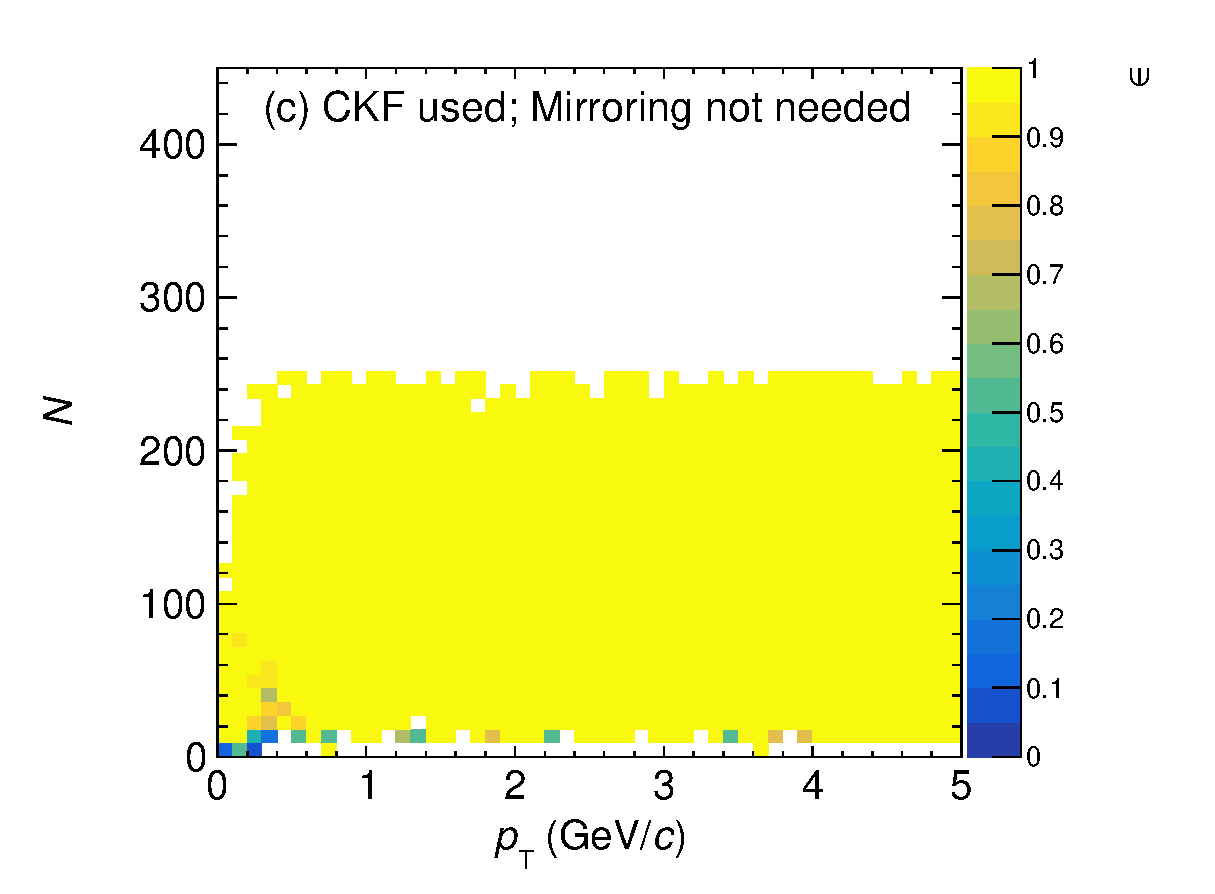
\includegraphics[width=\textwidth]{figures/ch5-KF_NDGAr/ToySample/ParScan/testNDGArMirrorEfficiencyVSNPointsVSpT_NoMirror.eps}
         \caption{}
         \label{fig:PS_Eff_CKF_NoMirror}
     \end{subfigure}
     \begin{subfigure}[b]{0.48\textwidth}
         \centering
         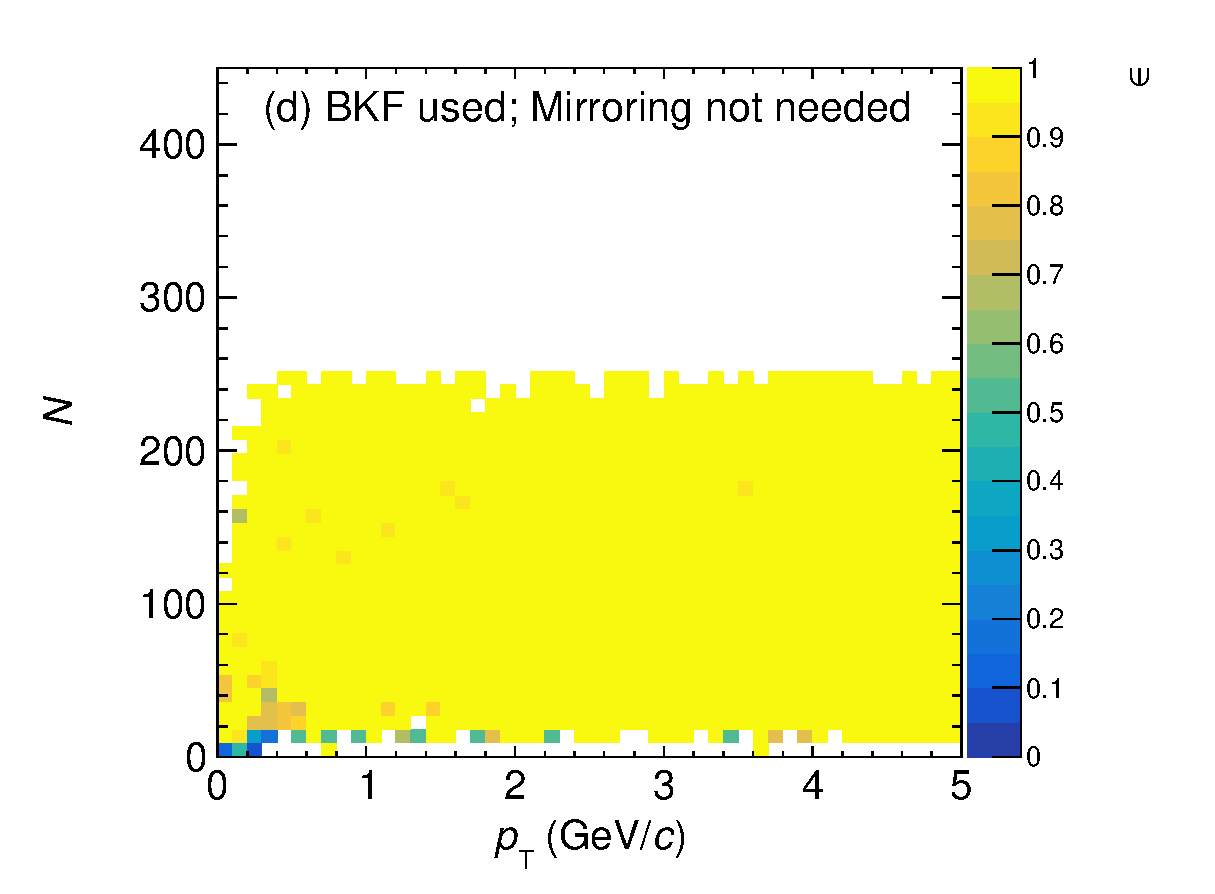
\includegraphics[width=\textwidth]{figures/ch5-KF_NDGAr/ToySample/ParScan/testNDGArMirrorEfficiencyVSNPointsVSpT_BKF_NoMirror.eps}
         \caption{}
         \label{fig:PS_Eff_BKF_NoMirror}
     \end{subfigure}
        \caption[Reconstruction efficiency $\epsilon$ for the PS sample.]{ Reconstruction efficiency $\epsilon$ for the PS sample, as a function of the total number of points in the track $N$ and the initial true transverse momentum $p_\textrm{T}$. The results for the tracks to which the mirroring technique was applied are shown in (a) and (c) for the \texttt{CKF} and \texttt{BKF} respectively. The results for the other tracks are shown in (c) for the \texttt{CKF} and (d) for the \texttt{BKF}.} \label{fig:PS_Eff}
\end{figure}


The difference in performance due to the mirror rotation can be quantified using the ratios between the full reconstruction resolution $\sqrt{C_{44}^{\textrm{CKF}}}$ and the $\sqrt{C_{44}^{\text{BKF}}}$ obtained with the basic reconstruction at a given point along the track. Figure~\ref{fig:SingleVSLeg_dens} shows the ratios $\sqrt{C_{44}^{\textrm{CKF}}}/\sqrt{C_{44}^{\text{BKF}}}$ as a function of the true $q/p_{\text{T}}$, color-coded according to the gas pressure $P_{\textrm{gas}}$. Figure~\ref{fig:SingleVSLeg_e} shows the results for a sample of only electrons, while Fig.~\ref{fig:SingleVSLeg_mu_pi} shows the results for a sample of muons and pions and Fig.~\ref{fig:SingleVSLeg_proton_kaon} for a sample of protons and kaons. The points are again randomly taken along the reconstructed tracks and down-sampled to $10\%$ of the total. For the electron sample, an overall relative improvement of $\sim 60\%$ is shown at $p_{\text{T}}<100$ MeV/$c$, with peaks of up to $\sim 80\%$ for the lowest momentum tracks in low pressure environments. This behavior is in agreement with Eqs.~\ref{eq:sigmaN} and~\ref{eq:sigmaMS} which show a dependency of the $1/p_{\text{T}}$ resolution on $1/\sqrt{N}$ and $1/\sqrt{L_\textrm{Arm}}$ respectively: using the mirroring technique, more space points of the tracks are used, resulting in larger $N$ and $L_\textrm{Arm}$. The dependence on the number of points is shown more clearly in Fig.~\ref{fig:SingleVSLeg_NPointsAll}, where the histograms are color coded for total number of points in the track, including those only accessible through the mirroring technique. Tracks containing more that 800 points are excluded for easier legibility of the results. It is shown that for the longest tracks, relative improvements of up to 80\% can be achieved. 


\begin{figure}[!ht]
     \centering
     \begin{subfigure}[h!]{0.9\textwidth}
         \centering
         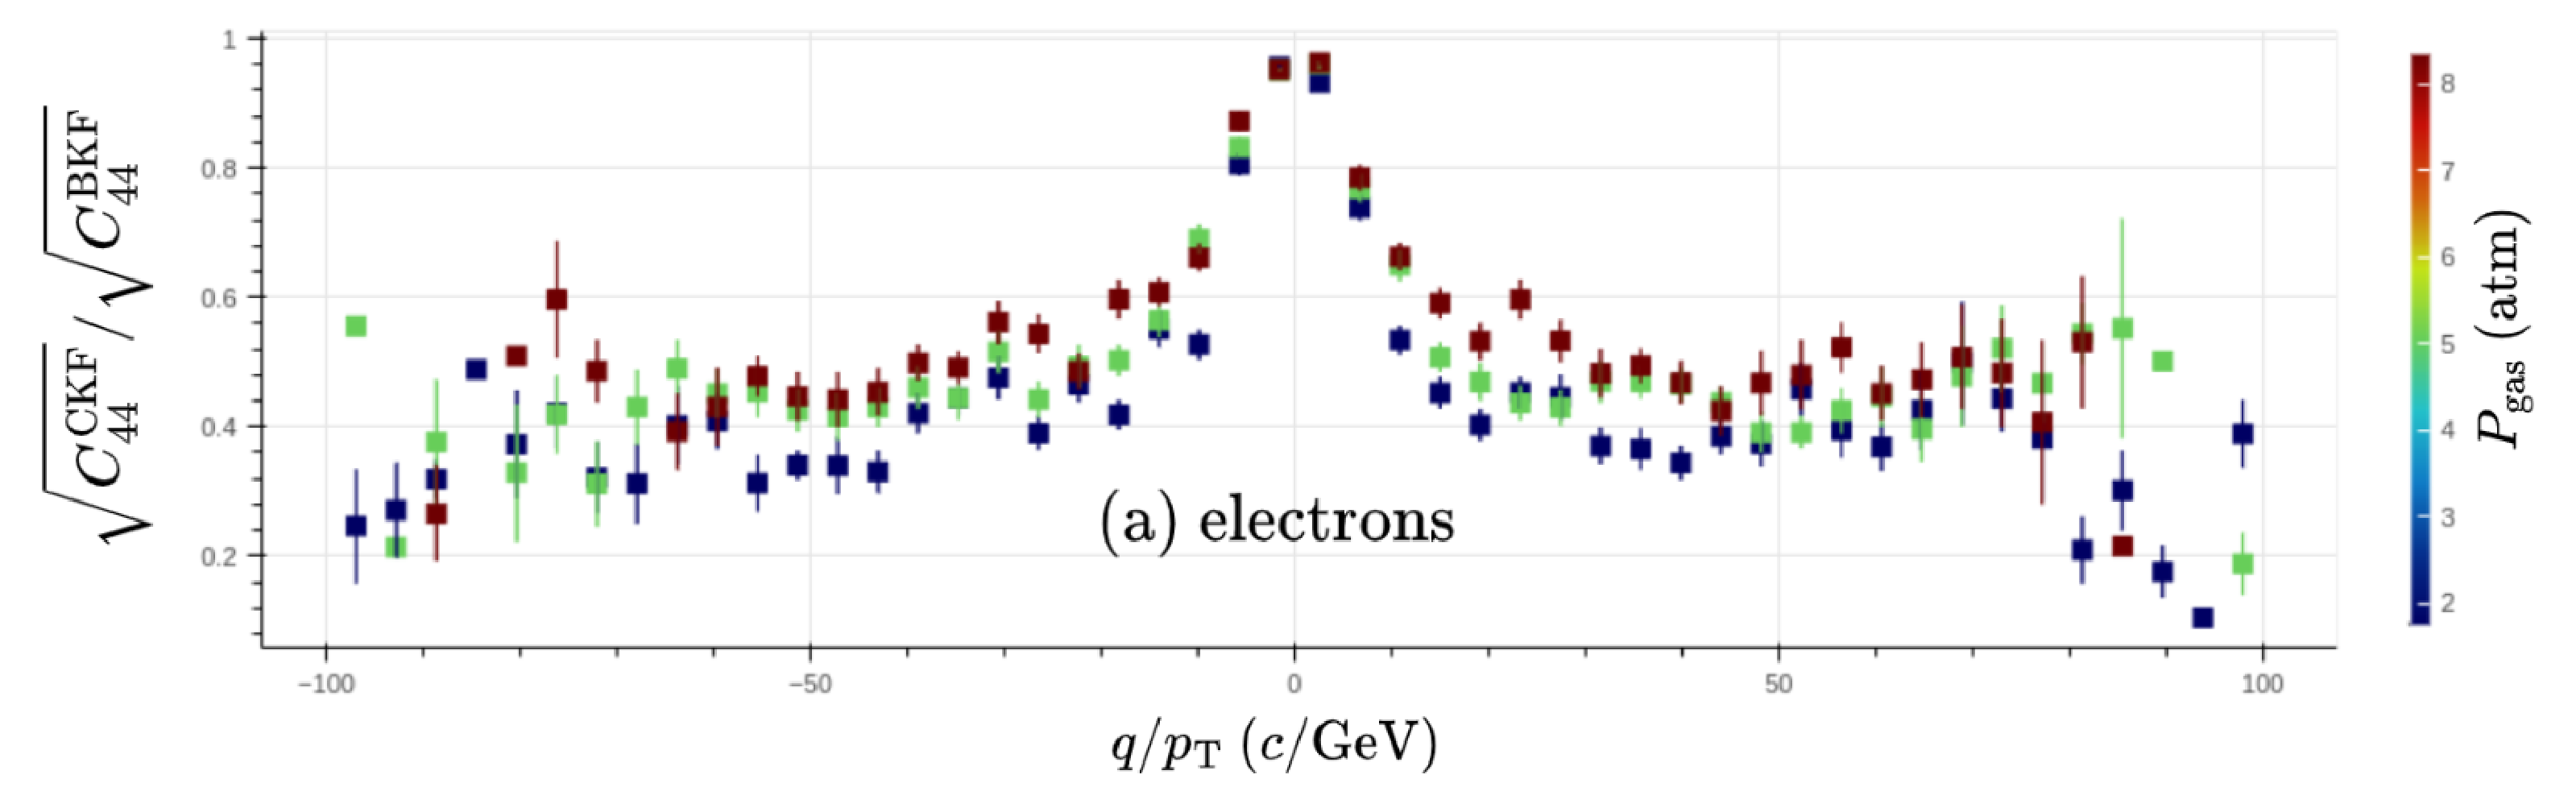
\includegraphics[width=\textwidth]{figures/ch5-KF_NDGAr/ToySample/ParScan/TotVSLegVSdens_11_label.eps}
         \caption{}
         \label{fig:SingleVSLeg_e}
     \end{subfigure}
     \begin{subfigure}[b]{0.9\textwidth}
         \centering
         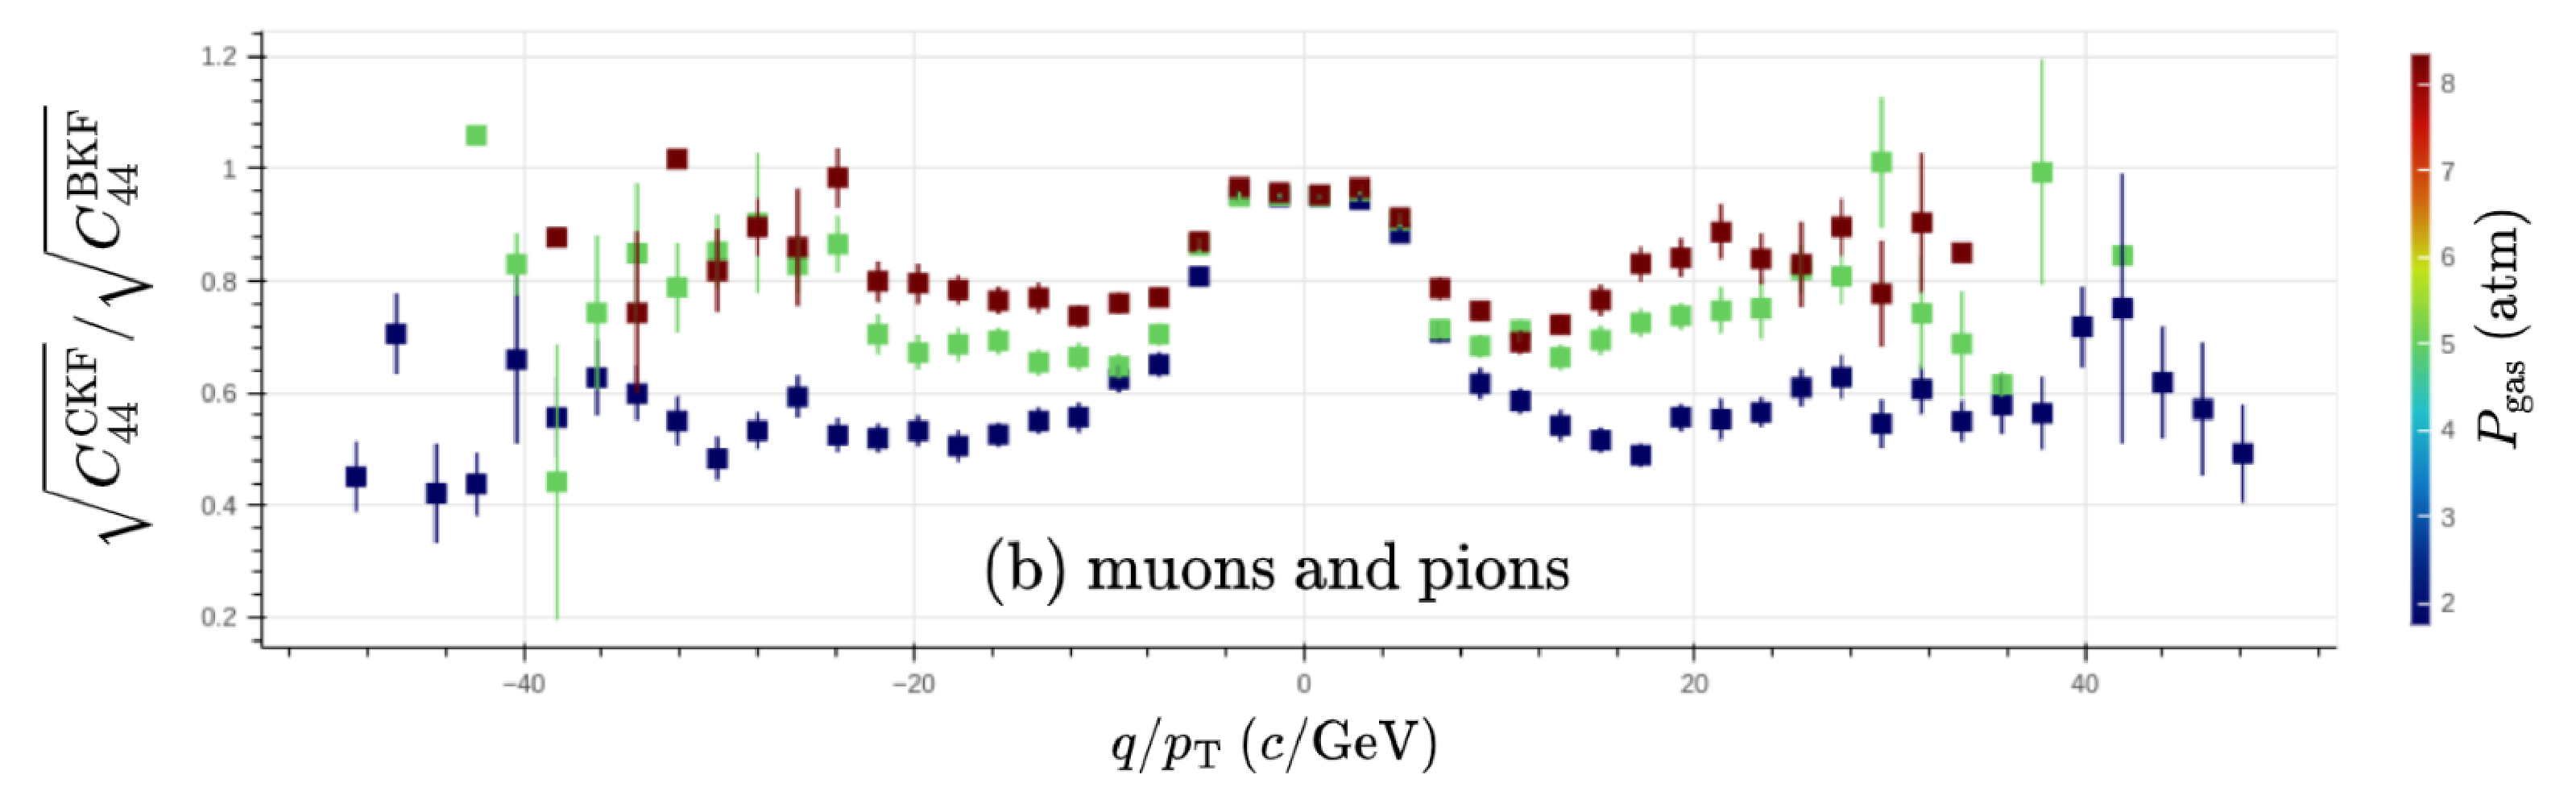
\includegraphics[width=\textwidth]{figures/ch5-KF_NDGAr/ToySample/ParScan/TotVSLegVSdens_13_211_label.eps}
         \caption{}
         \label{fig:SingleVSLeg_mu_pi}
     \end{subfigure}
          \begin{subfigure}[b]{0.9\textwidth}
         \centering
         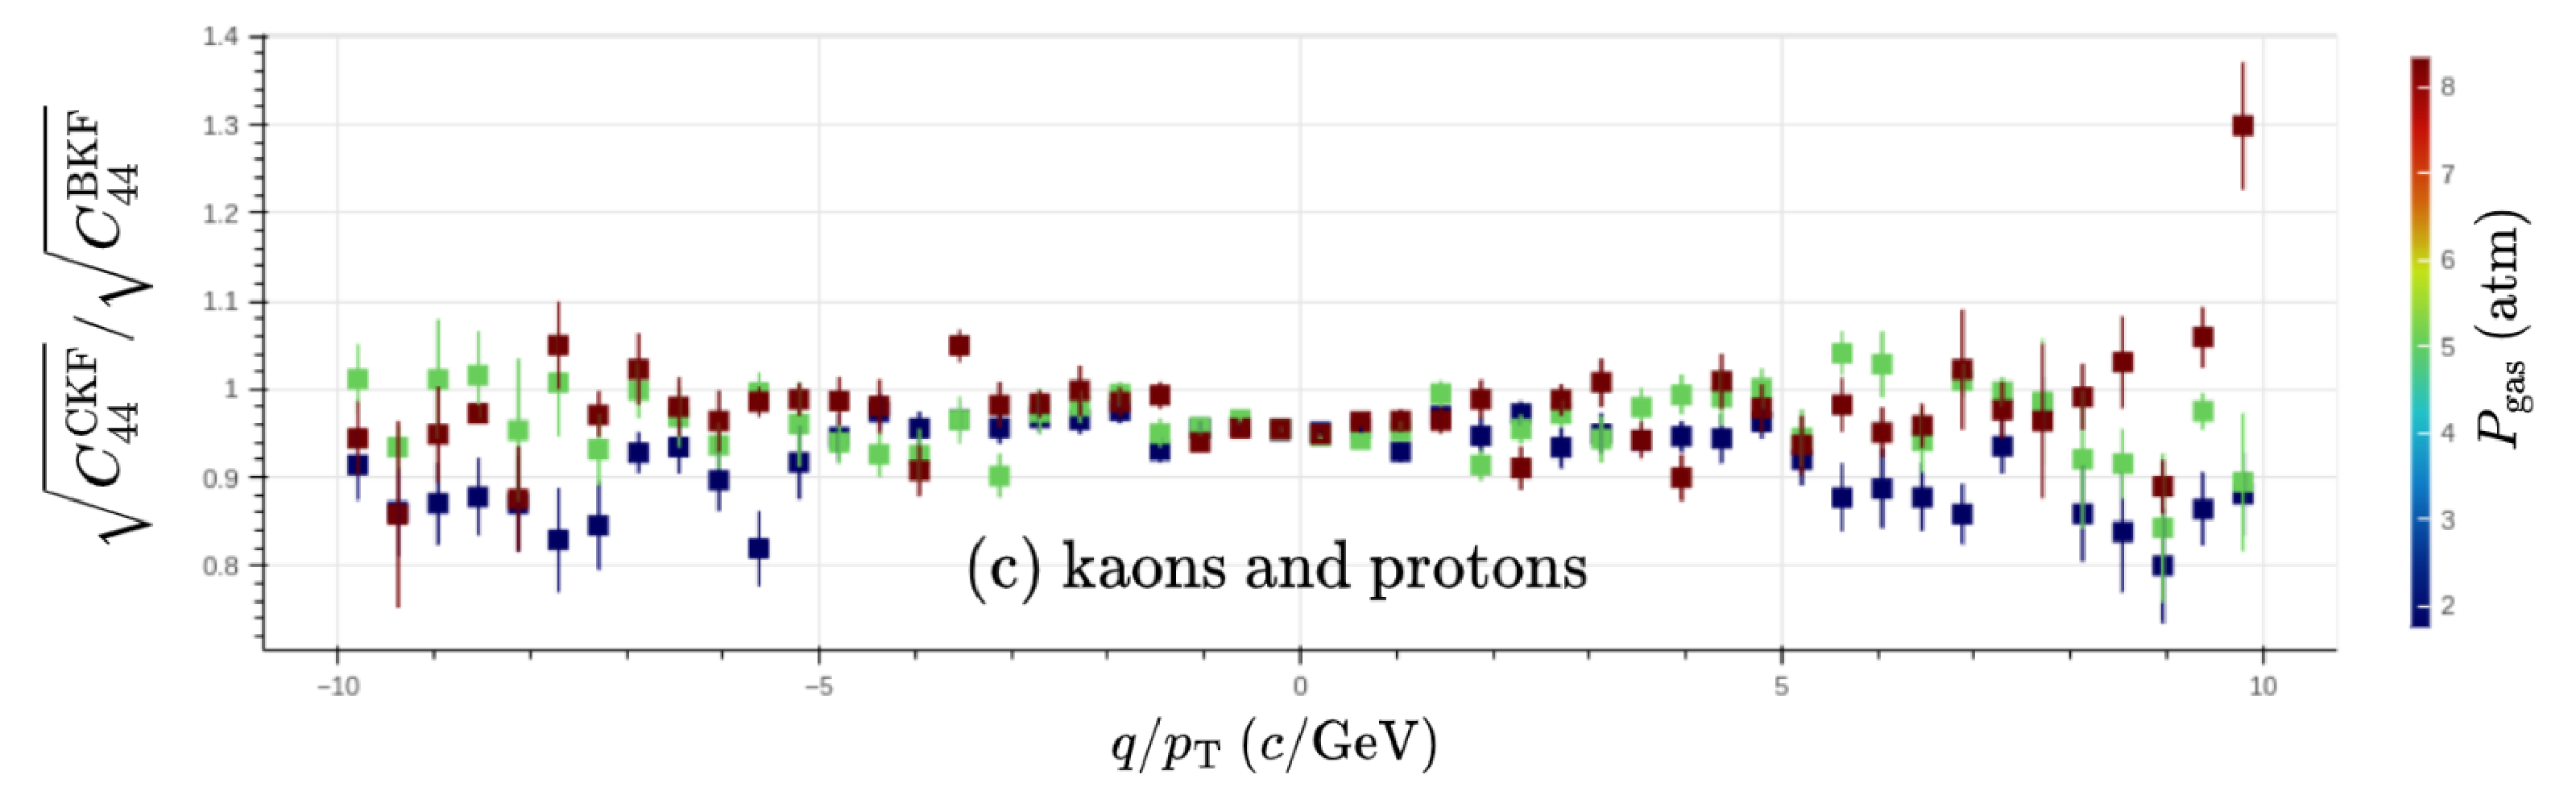
\includegraphics[width=\textwidth]{figures/ch5-KF_NDGAr/ToySample/ParScan/TotVSLegVSdens_2212_321_label.eps}
         \caption{}
         \label{fig:SingleVSLeg_proton_kaon}
     \end{subfigure}
        \caption[Ratios of the $q/p_\text{T}$ resolutions obtained using the full \texttt{CKF} algorithm including the mirror rotation method $\sqrt{C_{44}^{\textrm{CKF}}}$, over the reconstruction without mirror rotation $\sqrt{C_{44}^{\text{BKF}}}$.]{Ratios of the $q/p_\text{T}$ resolutions obtained using the full \texttt{CKF} algorithm including the mirror rotation method $\sqrt{C_{44}^{\textrm{CKF}}}$, over the reconstruction without mirror rotation $\sqrt{C_{44}^{\text{BKF}}}$. The plots were produced for the whole PS sample. The histograms are color coded according to the gas pressure $P_{\textrm{gas}}$. Plot (a) contains only electrons, plot (b) contains pions and muons and plot (c) contains kaons and protons. Only tracks with a minimum of 30 points are considered. These plots have been produced using the interactive analytical tool \texttt{ROOTInteractive}~\cite{RootInt}. The error bars are statistical.}
        \label{fig:SingleVSLeg_dens}
\end{figure}
\begin{figure}[!ht]
     \centering
     \begin{subfigure}[h!]{0.99\textwidth}
         \centering
         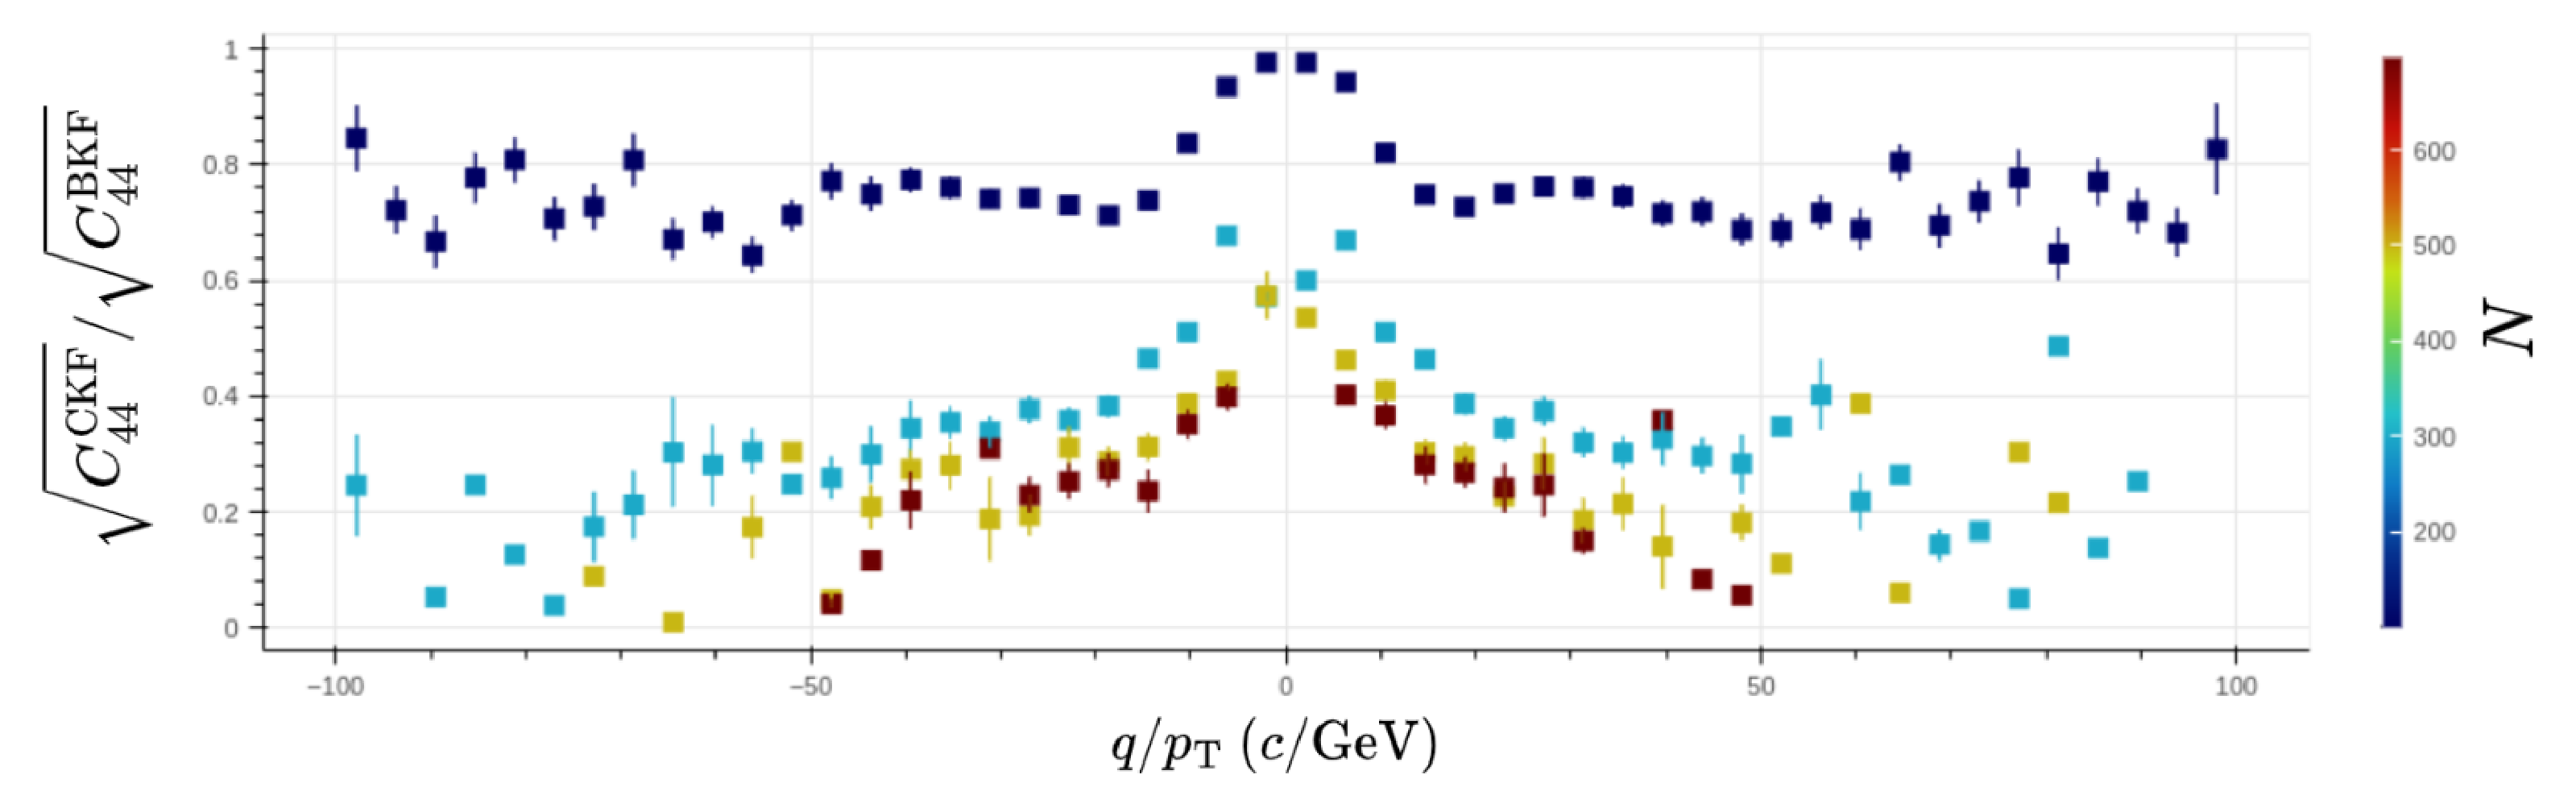
\includegraphics[width=\textwidth]{figures/ch5-KF_NDGAr/ToySample/ParScan/TotVSLegVSNPoints_label.eps}
         \caption{}
         \label{fig:SingleVSLeg_NPoints}
     \end{subfigure}
        \caption[Similar plot to Fig.~\ref{fig:SingleVSLeg_dens}. The plot contains all particle types in the PS sample. The histograms are color coded according to the number of points in the track $N$.]{Similar plot to Fig.~\ref{fig:SingleVSLeg_dens}. The plot contains all particle types in the PS sample. The histograms are color coded according to the number of points in the track $N$.}
        \label{fig:SingleVSLeg_NPointsAll}
\end{figure}

The difference between the results is shown to be less dramatic in more pressurized environments, where particles tend to be absorbed sooner and tracks are generally shorter. This trend is confirmed looking at the results obtained for the muons and pions sample in Fig.~\ref{fig:SingleVSLeg_mu_pi}, for which $\textrm{d}E/\textrm{d}x$ will on average be higher due to their higher masses: the improvement in this case is by $\sim 20\%$ for $p_{\text{T}}<150$ MeV/$c$ with peaks of up to $\sim50$\% for the lowest momentum tracks in low pressure environments. No improvements were found for the more massive particles shown in the sample, except for minor ones at lower pressures (Fig.~\ref{fig:SingleVSLeg_proton_kaon}).


\subsection{The high pressure study}
\label{Sec:HPSample}
The HP sample is used to evaluate the detector performance of a HPgTPC similar to ND-GAr. We focus on the total momentum relative resolution and bias, defined as the $\sigma$ and $\mu$ of a standard Gaussian fit applied to the momentum fractional residuals:
\begin{equation}
    R = \frac{p_{\text{reco}}}{p_{\text{true}}} - 1.
\end{equation}
The reconstruction efficiency $\epsilon$ was also tested. The results are shown in the App. \ref{App:MoreNDGAr} in Fig. \ref{fig:HP_Eff} and are similar to the PS Sample.

\begin{figure}[!ht]
     \centering
     \begin{subfigure}[b]{0.49\textwidth}
         \centering
         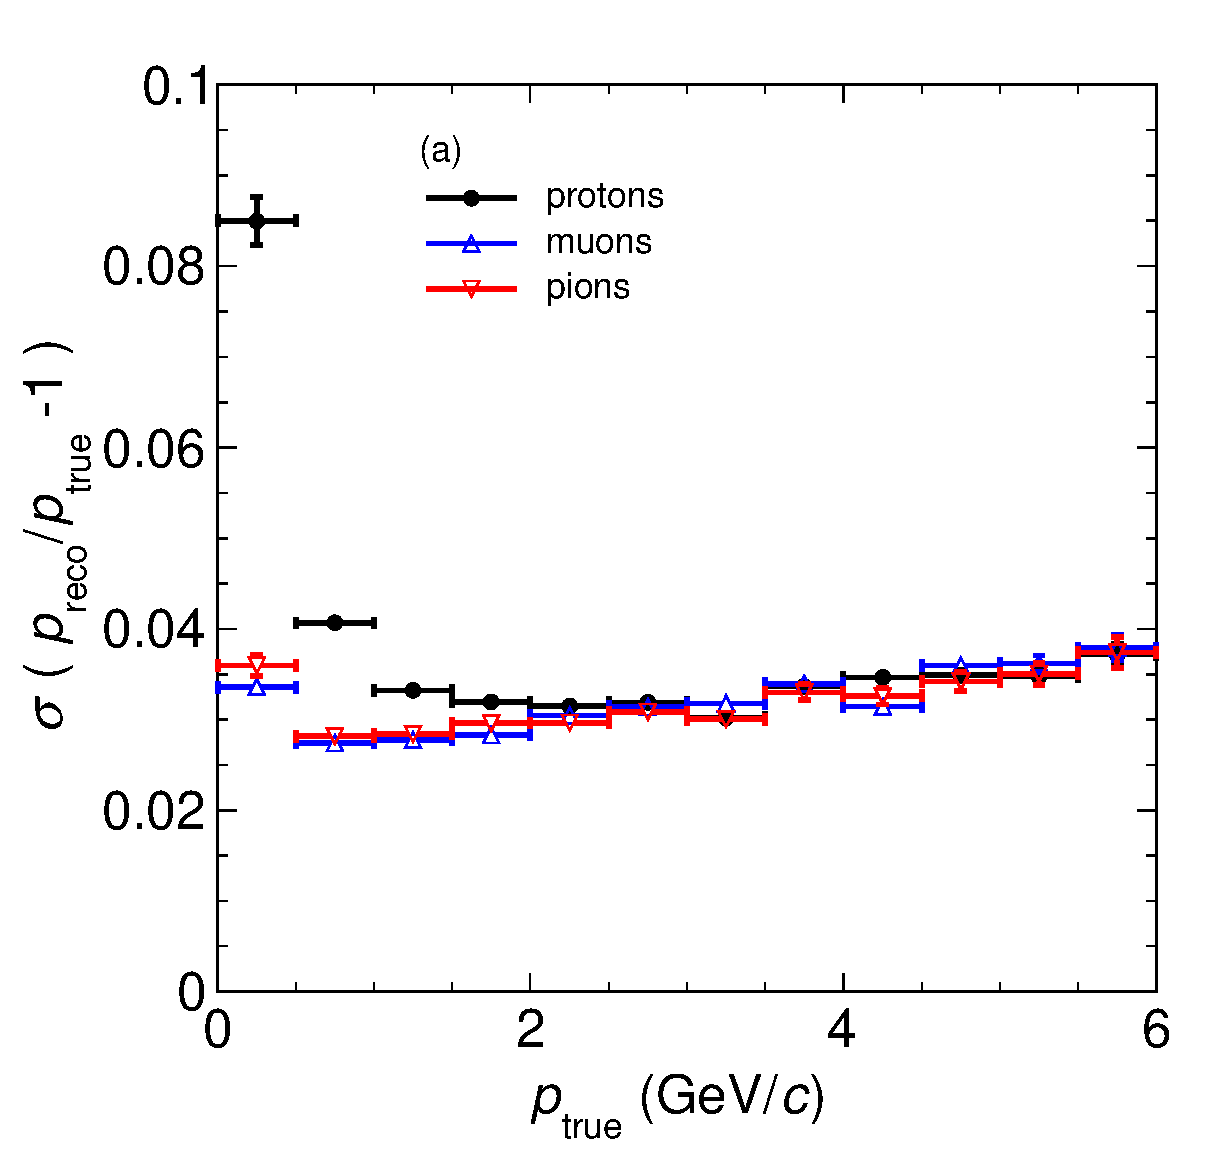
\includegraphics[width=\textwidth]{figures/ch5-KF_NDGAr/ToySample/HighPres/RespVSp_XL.eps}
         \caption{}
         \label{fig:ResND-GArVSp}
     \end{subfigure}
     \begin{subfigure}[b]{0.49\textwidth}
         \centering
         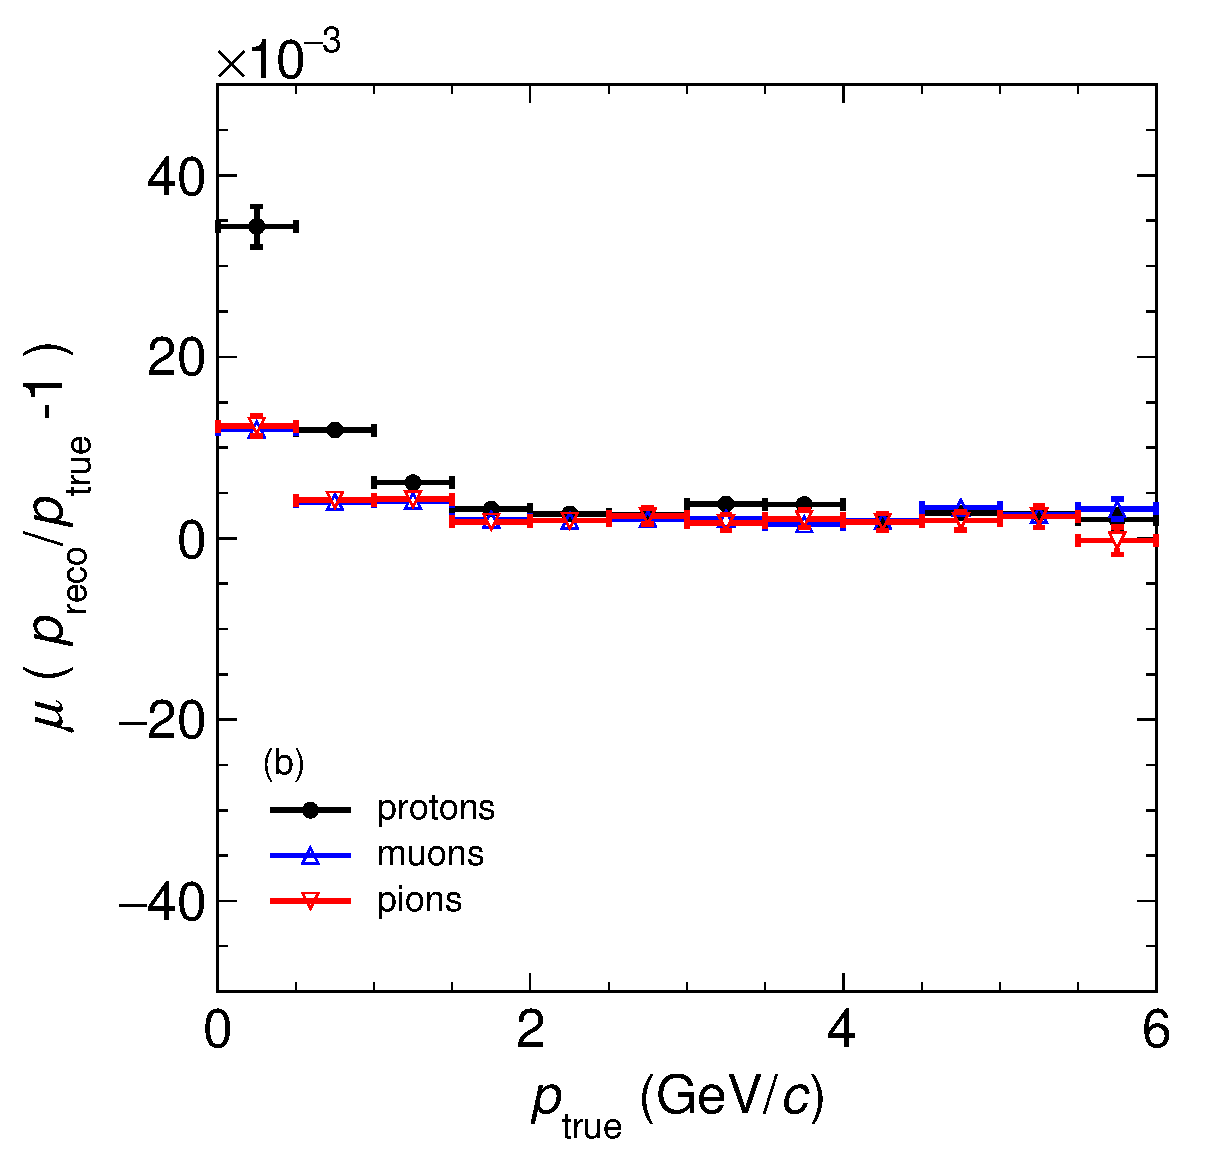
\includegraphics[width=\textwidth]{figures/ch5-KF_NDGAr/ToySample/HighPres/BiaspVSp_XL.eps}
         \caption{}
         \label{fig:BiasND-GArVSp}
     \end{subfigure}
        \caption[Relative momentum resolution (a) and bias (b) as function of the true momentum, $p_\textrm{true}$, for the HP sample.]{Relative momentum resolution (a) and bias (b) as function of the true momentum, $p_\textrm{true}$, for the HP sample. The two properties are defined as $\mu$ and $\sigma$ of Gaussian fits of the momentum fractional residuals $p_{\text{reco}}/p_{\text{true}}-1$. The three particle types (protons, muons and pions) are drawn separately.}
        \label{fig:ND-GArVSp}
\end{figure}

\begin{figure}[!ht]
     \centering
     \begin{subfigure}[b]{0.49\textwidth}
         \centering
         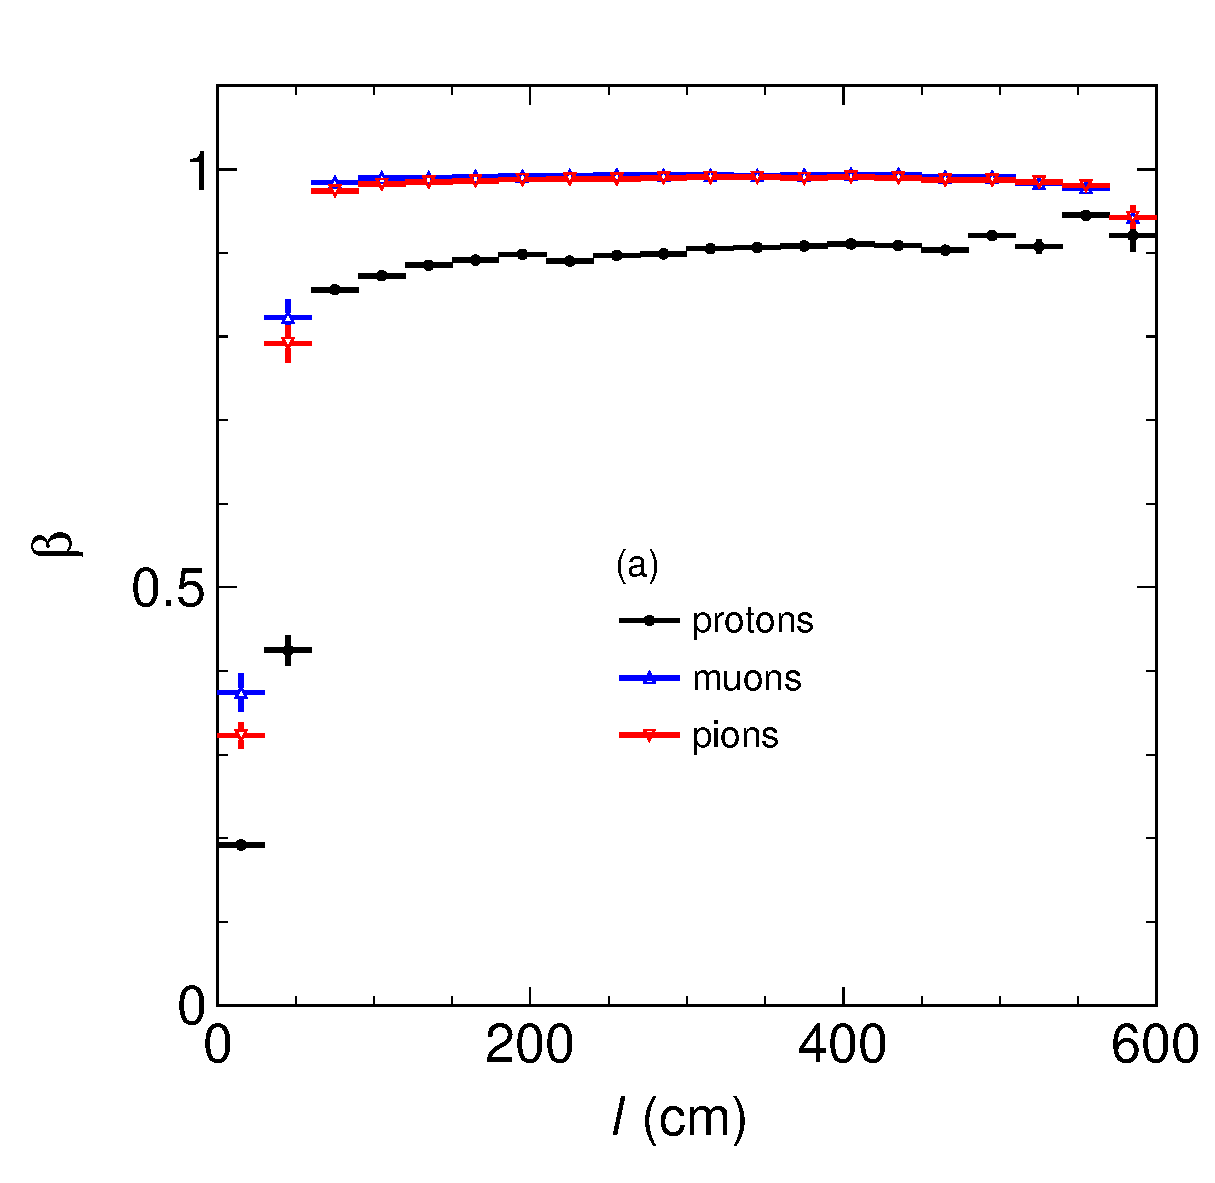
\includegraphics[width=\textwidth]{figures/ch5-KF_NDGAr/ToySample/HighPres/testNDGArMirrorbetaVSl.eps}
         \caption{}
         \label{fig:betaVSlength}
     \end{subfigure}
     \begin{subfigure}[b]{0.49\textwidth}
         \centering
         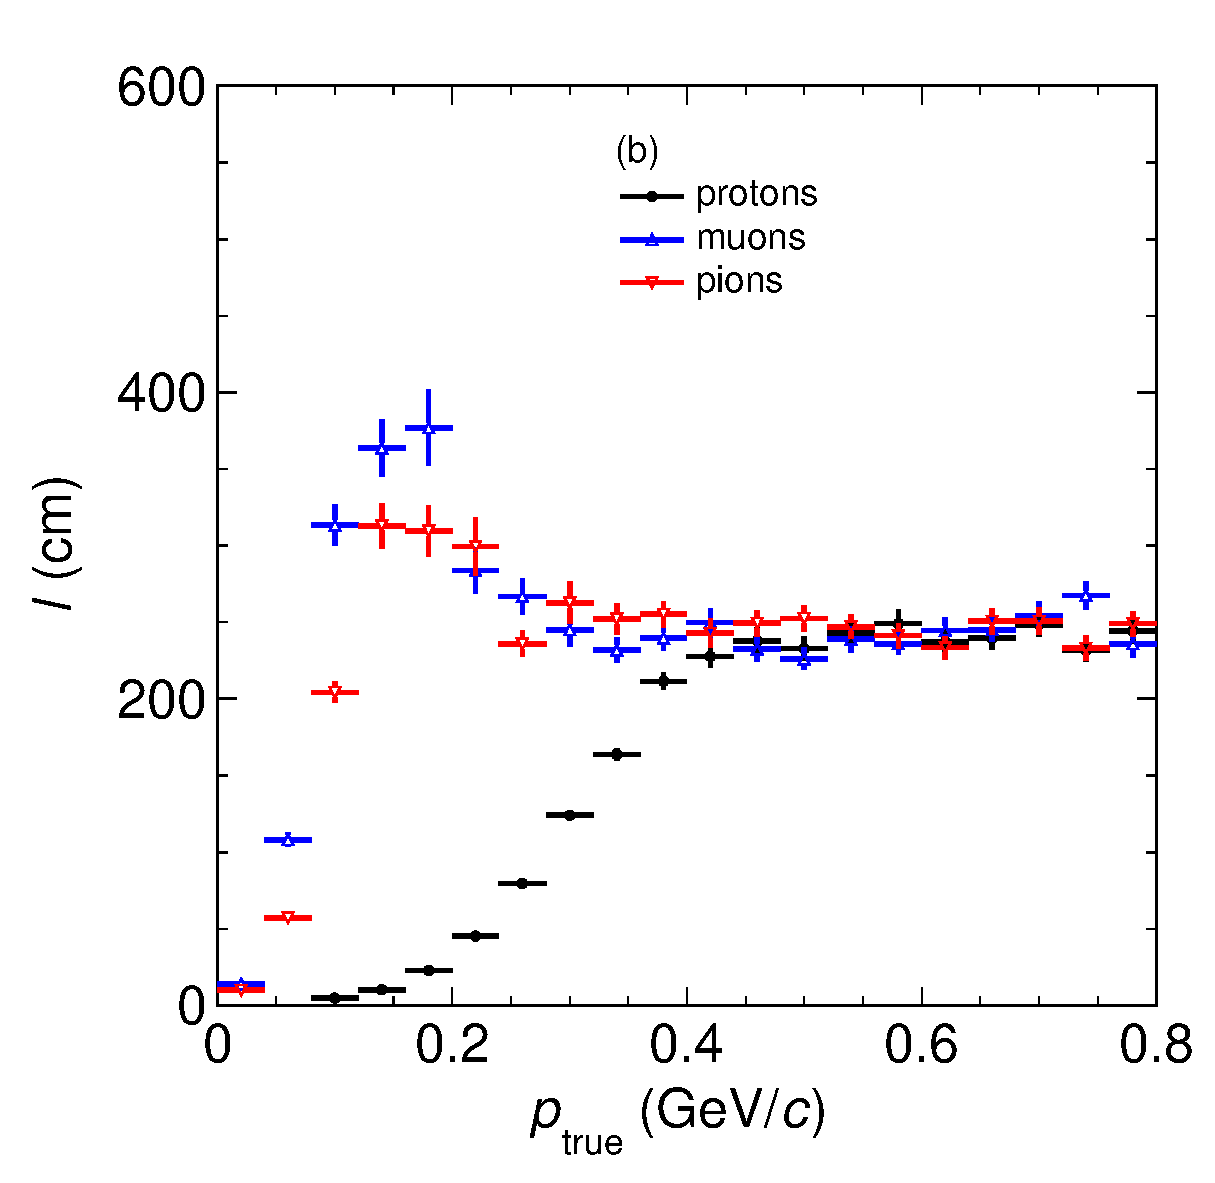
\includegraphics[width=\textwidth]{figures/ch5-KF_NDGAr/ToySample/HighPres/testNDGArMirrorLengthVSp.eps}
         \caption{}
         \label{fig:lengthVSp}
     \end{subfigure}
        \caption{(a) Average $\beta$ as a function of the track length $l $ and  (b) average track length as a function of the true momentum $p_\textrm{true}$ for the HP sample.}
        \label{fig:ND-GArextraprops}
\end{figure}

The dependencies of the total momentum resolution can be described using Eqs. \ref{eq:sigmaNptot} and \ref{eq:sigmaMSptot}. In Fig.~\ref{fig:ND-GArVSp} we show the relative momentum resolution and bias as a function of the true momentum for the three particle types present in the sample. At lower momenta ($p_{\text{true}}<1\text{GeV/}c$) the resolution is close to 2\% for pions and muons while it is closer to 8\% for the protons. In this momentum region the multiple scattering component of the resolution is dominant. This component is inversely proportional to the particles' $\beta$ factor. With a given momentum, the proton, having a higher mass, will always have a smaller $\beta$ and thus a worse expected resolution. Furthermore, while muons and protons at lower energies have the chance to produce longer and even looping tracks inside the detector, protons will tend to loose their energy more quickly, again due to their masses. This is clearly shown in Fig.~\ref{fig:lengthVSp} where the average particle lengths as a function of their true momentum is shown. Somewhat significant biases are also shown at these lower momenta, especially for protons. For momenta $p_{\text{true}}>1~\text{GeV/}c$, the resolution is comparable for the three particle types and increases slowly with the particle momentum. At higher momenta the point resolution component is dominant, so a direct proportionality on the momentum is expected, with no distinction between the particle types. An inverse dependency on the lever arm and number of points and thus indirectly on the length is also expected, but as shown in Fig.~\ref{fig:lengthVSp}, in this momentum range the average length of the track becomes roughly the same for all particle types.

\begin{figure}[!ht]
     \centering
     \begin{subfigure}[b]{0.49\textwidth}
         \centering
         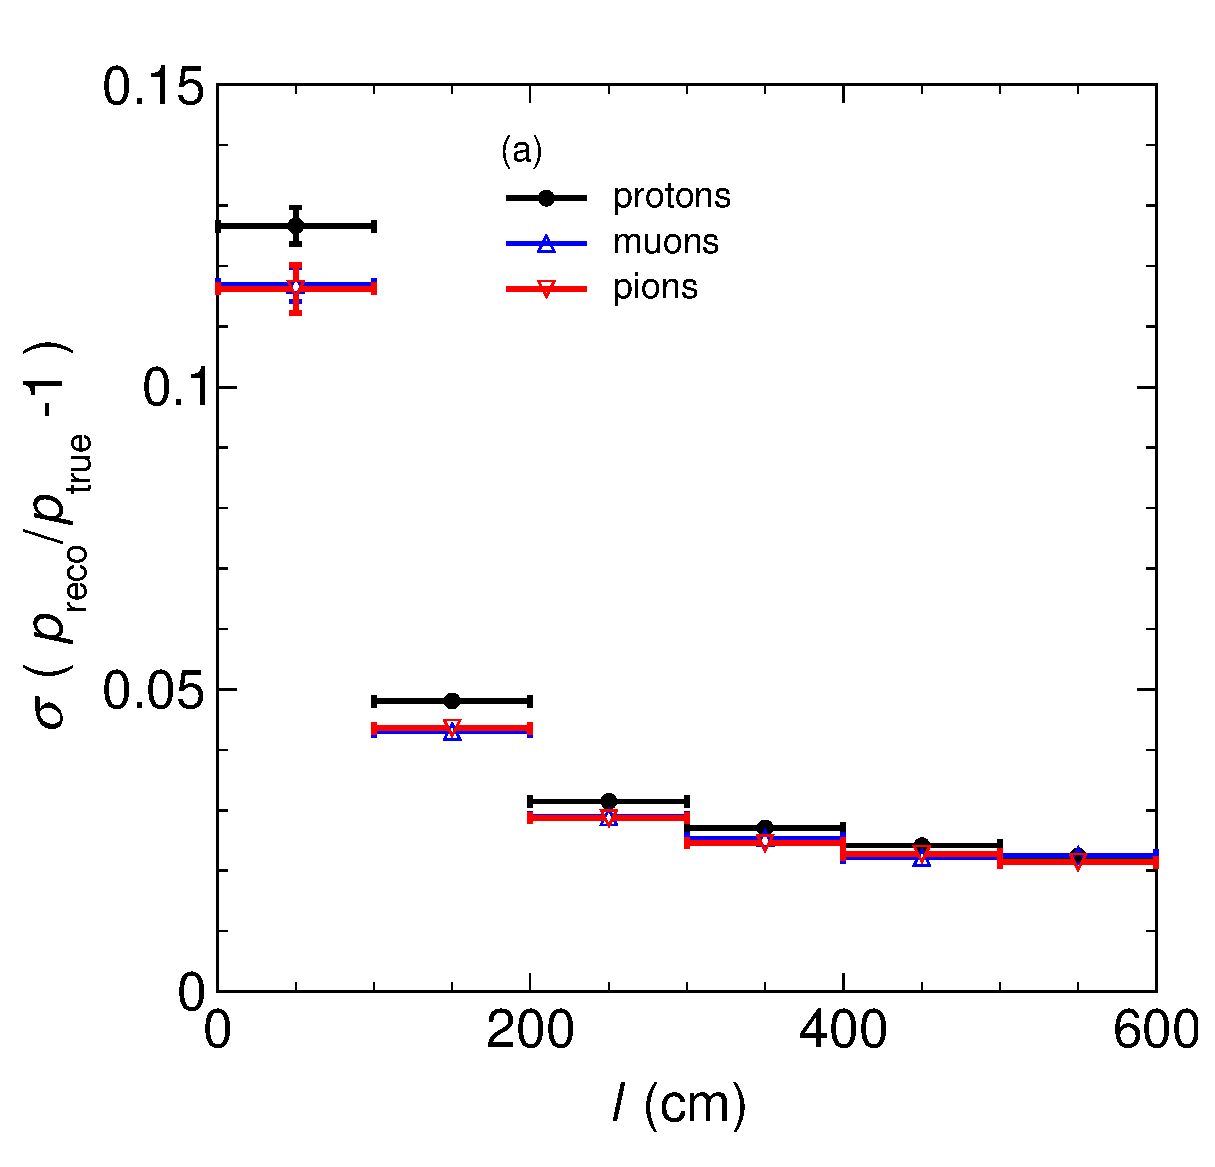
\includegraphics[width=\textwidth]{figures/ch5-KF_NDGAr/ToySample/HighPres/RespVSLength_XL.eps}
         \caption{}
         \label{fig:ResND-GArVSlength}
     \end{subfigure}
     \begin{subfigure}[b]{0.49\textwidth}
         \centering
         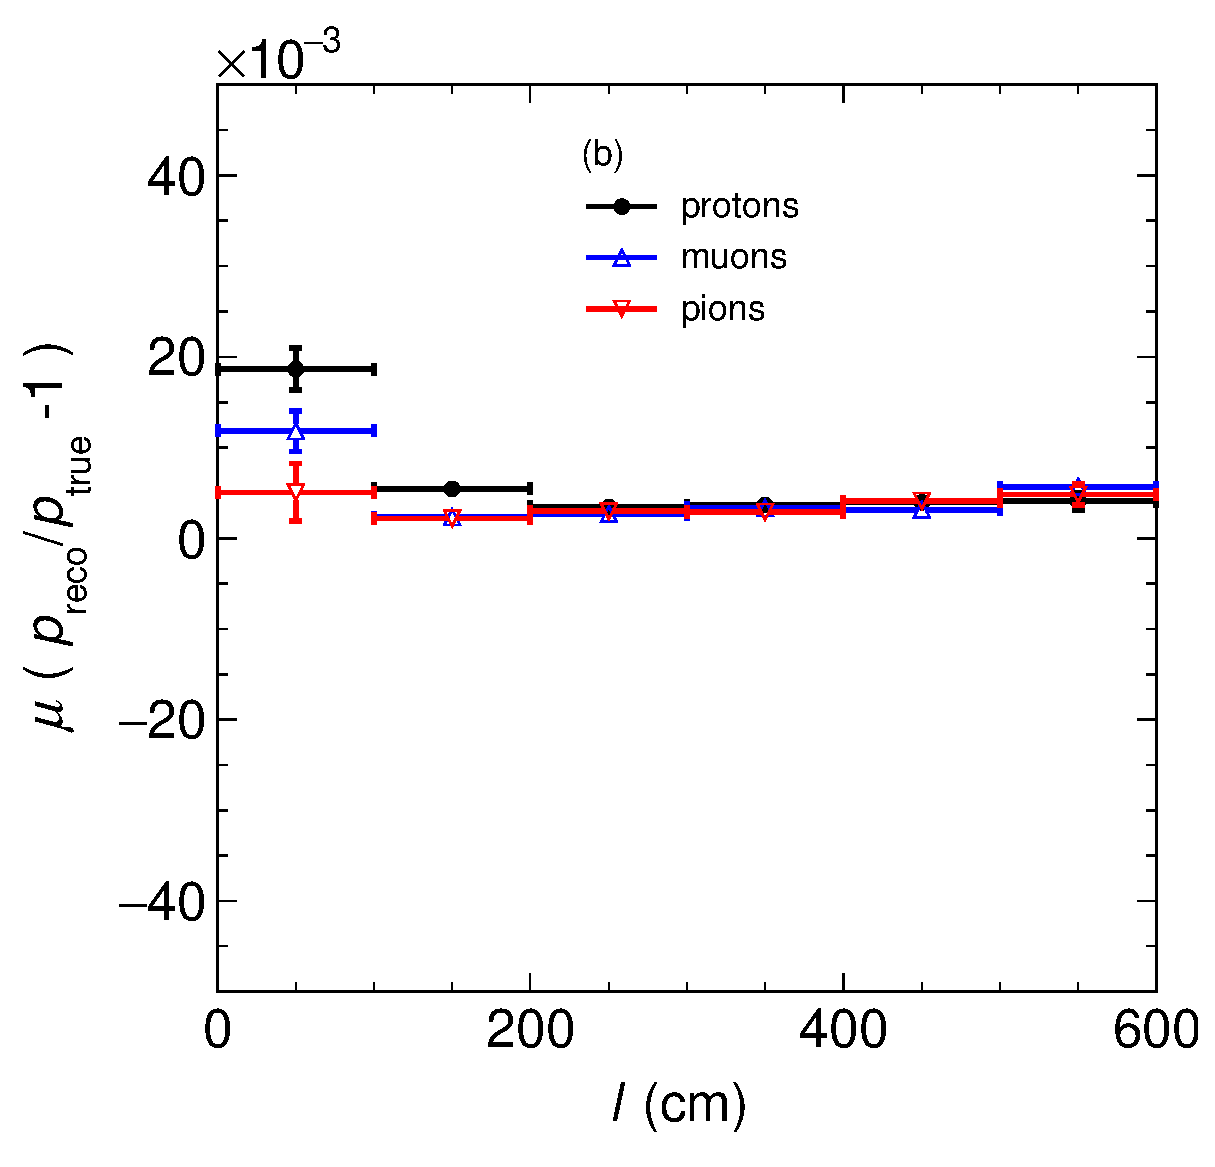
\includegraphics[width=\textwidth]{figures/ch5-KF_NDGAr/ToySample/HighPres/BiaspVSLength_XL.eps}
         \caption{}
         \label{fig:BiasND-GArVSlength}
     \end{subfigure}
        \caption{Similar plots to Fig.~\ref{fig:ND-GArVSp}. In this case the relative momentum resolution (a) and bias (b) are shown as a function of the true track length $l$ for the HP sample.}
        \label{fig:ND-GArVSlength}
\end{figure}

In Fig.~\ref{fig:ND-GArVSlength} we show the momentum resolution and bias as a function of the true track lengths $l$ for the three particle types. As could be predicted from Eq.~\ref{eq:sigmaMSptot}, an inverse proportionality of the relative resolution on $l$ can be observed for all particle types. The worse performance observed for the protons can be explained by the average $\beta$ shown in Fig.~\ref{fig:betaVSlength}, which is always smaller for more massive particles regardless of the length of the tracks. For longer tracks the hit component of the resolution is dominant and the difference in $\beta$ is not as impactful. A somewhat significant bias can be seen at lower lengths. Similar dependencies on lever arm $L_{\textrm{Arm}}$ and number of points in the track $N$, which can be treated as a proxy for $l$ in most cases, are shown in Figs.~\ref{fig:ND-GArVSLArm} and~\ref{fig:ND-GArVSNPoints} in the App. \ref{App:MoreNDGAr}.



\section{Implementation in \texttt{GArSoft}}
\label{Sec:Garsoft_Implementation}
The \texttt{GArSoft} software suite was used to produce samples of $\nu_\mu$ CC interactions inside the the ND-GAr TPC via the GENIE Monte Carlo generator. A second sample of forward going muons was produced using the GEANT4 based particle gun feature of \texttt{GArSoft}.

The first sample was used to extrapolate particle tracks produced by primary protons, muons and pions. The \texttt{CKF} algorithm was applied to the track candidates produced by \texttt{GArSoft} and its performance was compared to that of the \texttt{GKF} in terms of total momentum and angle resolution. The sample was also used to confirm the internal consistency of the algorithm already demonstrated using \texttt{fastMCKalman}. We will refer to this as the interaction sample. The particle gun sample was used to estimate the performance of the new algorithm with particle tracks reproducing the conditions of muons coming from the ND-LAr detector, which is one of the key samples of study in ND-GAr.

The \texttt{CKF} algorithm which was tested on these \texttt{GArSoft} produced samples is identical to the one discussed in Sec. \ref{Sec:KalGAr} and tested using \texttt{fastMCKalman} in Sec. \ref{Sec:ToyMCStudy_GAr} expect for the choice of the rotation center. While for the algorithm tested so far the rotation center was chosen to be fixed at the center of the TPC chamber, in this new application it is placed in front of the particle track. Specifically a simple linear fit is applied to the first 10 points of the track, and the rotation center is chosen to be 30 cm away from the first point along the fitted line. This choice was made to avoid the unnecessary use of the mirroring technique, especially in the case of forward going tracks. In these scenarios the particle trajectories are often parallel to track pad layers for large portions of their trajectories and the application of the mirroring technique would produce large jumps, inducing the loss of hit clusters and a worse performance overall. This feature couldn't be seen when using the \texttt{fastMCKalman} Toy MC generator, because in that case the mirroring technique was used in the simulation as well as in the reconstruction, producing gaps in the tracks themselves. Imposing that the rotation center is put in front of the start of the track, we reduce the application of the mirroring technique to very \enquote{bendy} and often looping tracks, for which the method is always beneficial, adding hit clusters that wouldn't have been available otherwise. 

Another less significant difference exists in the application of the \texttt{Seed} algorithm. While for the tests performed using the \texttt{fastMCKamlman} algorithm, a limit of 60 points was imposed on the length of the track segment used for the seeding, in this case the entire track is always used. This choice was made in order to obtain the highest precision possible in the estimation of the state vector parameters, but it has the side effect of making the estimation of the covariance matrix less reliable, especially when it comes to the energy loss and multiple scattering effects. However the additional precision in the state vector estimates yielded better results during the testing stage. Similarly to what was done for the HP sample in Sec. \ref{Sec:HPSample} the Energy Loss and Multiple Scattering corrections were evaluated by considering the characteristics of a 90-10 Ar-CH$_4$ gas mixture and then scaling them by a 10 atm pressure factor.

Once the \texttt{CKF} algorithm was fully mature and proven to outperform the \texttt{GKF}, it was implemented into \texttt{GArSoft} and set as the standard fitter. Additional tests were performed using two $\nu_\mu$ CC interaction samples, produced entirely in \texttt{GArSoft}, using the same simulation up to the signal formation and digitization step but then using the two different fitters for the reconstruction. These samples were used to test that the integrated \texttt{CKF} fitter would behave identically to original independent code. Furthermore, they were utilized to compare aspects of the performance of the two fitters that would have been difficult to test prior to the full integration, such as reconstruction efficiency and vertexing resolution. 

\subsection{The interaction sample}
\label{sec:interactionGAr}

\begin{figure}[t]
     \centering
     \begin{subfigure}[b]{0.48\textwidth}
         \centering
         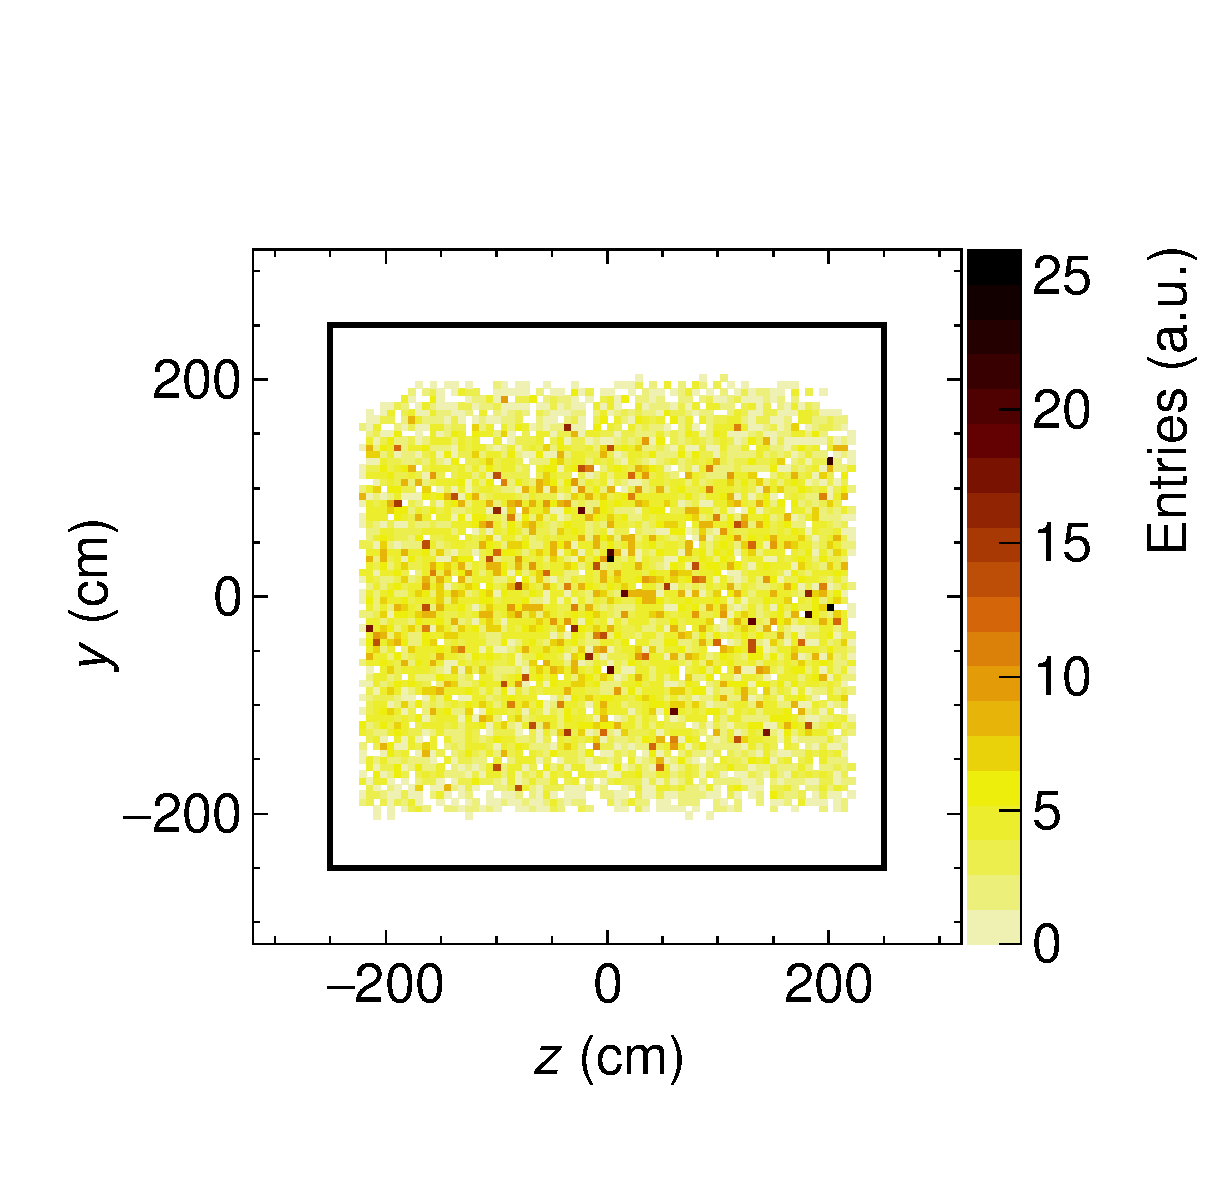
\includegraphics[width=\textwidth]{figures/ch5-KF_NDGAr/FullSample/Int/Props/YZ_view.eps}
         \caption{}
         \label{fig:YZViewGArInt}
     \end{subfigure}
     \begin{subfigure}[b]{0.48\textwidth}
         \centering
         \includegraphics[width=\textwidth]{figures/ch5-KF_NDGAr/FullSample/Int/Props/XY_view.eps}
         \caption{}
         \label{fig:XYViewGAr_Int}
     \end{subfigure}
        \caption[Starting positions for secondary particles in the interaction sample.]{Starting positions for secondary particles in the interaction sample. The left plot shows the distribution in the $zy$ plane, while the plot on the right shows the distribution in the $xy$ plane. The edges of the TPC are drawn on top. } \label{fig:ViewGArInt}
\end{figure}

To study the performance of the \texttt{CKF} we produced a sample composed of primary particles from $5\times10^4$  $\nu_\mu$ CC interactions inside the ND-GAr detector's TPC area. This was done using the GENIE neutrino interaction MC generator through \texttt{GArSoft}, propagating the particles using Geant4 and following all the simulation steps outlined in Sec. \ref{Sec:GArSoft-GAr}. We'll refer to this sample simply as the interaction sample. From the sample we selected protons, pions and muons and applied a fiducial cut on the true interaction vertices, imposing that they lie at least 20 cm from the barrel sides and 10 cm from the end-caps. This was done to eliminate many potentially problematic short tracks. The true vertex positions of all the events selected from the sample are shown in Fig. \ref{fig:ViewGArInt}.

\begin{figure}[t]
     \centering
     \begin{subfigure}[b]{0.32\textwidth}
         \centering
         \includegraphics[width=\textwidth]{figures/ch5-KF_NDGAr/FullSample/Int/Props/pTAllTall.eps}
         \caption{}
         \label{fig:ptTPC_Int}
     \end{subfigure}
     \begin{subfigure}[b]{0.32\textwidth}
         \centering
         \includegraphics[width=\textwidth]{figures/ch5-KF_NDGAr/FullSample/Int/Props/LArmTall.eps}
         \caption{}
         \label{fig:LTPC_Int}
     \end{subfigure}
          \begin{subfigure}[b]{0.32\textwidth}
         \centering
         \includegraphics[width=\textwidth]{figures/ch5-KF_NDGAr/FullSample/Int/Props/NTall.eps}
         \caption{}
         \label{fig:NTPC_Int}
     \end{subfigure}
        \caption[Distributions of key track quantities in the interaction sample]{Distributions of (a) transverse momentum $p_{\textrm{T}}$,  (b) lever arm $L_{\textrm{Arm}}$ and (c) number of points per track $N$ in the interaction sample sample. In all the plots the distributions for muons, pions and protons are shown separately. } \label{fig:TPCProperties_Int}
\end{figure}


Some key features of the particle tracks are shown in Fig. \ref{fig:TPCProperties_Int}. The histograms are separated between the different particle types (i.e. muons, pions and protons) of the true particles matched to the tracks by the \texttt{GArSoft} back-tracker. We show the true initial transverse momentum $p_\text{T}$ in the $xy$ plane, the number of hit clusters belonging to the tracks $N$ and the lever arm $L_\textrm{Arm}$, defined as the distance between the first and last track point in the $xy$ plane. As expected from $\nu_\mu$ CC interactions, where most of the initial neutrino momentum is transferred to the exiting muon, the muon sample has a higher momentum distribution compared to protons and pions. It is interesting to notice that significant $L_\text{Arm}$ and $N$ peaks are present in the lower regions of the spectra. While some of these shorter tracks are produced by particles stopping in the detector, especially in the case of protons, many of them are also the product of errors in the track formation stage of \texttt{GArSoft}. These errors include clumps of hits produced by $\delta$ rays that are wrongly assigned to a true MC particle by the back-tracker or longer tracks that are cut into shorter segments.

\begin{figure}[t]
     \centering
     \begin{subfigure}[b]{0.32\textwidth}
         \centering
         \includegraphics[width=\textwidth]{figures/ch5-KF_NDGAr/FullSample/Int/Props/ResX.eps}
         \caption{}
         \label{fig:TPCXRes_Int}
     \end{subfigure}
     \begin{subfigure}[b]{0.32\textwidth}
         \centering
         \includegraphics[width=\textwidth]{figures/ch5-KF_NDGAr/FullSample/Int/Props/ResY.eps}
         \caption{}
         \label{fig:TPCYRes_Int}
     \end{subfigure}
          \begin{subfigure}[b]{0.32\textwidth}
         \centering
         \includegraphics[width=\textwidth]{figures/ch5-KF_NDGAr/FullSample/Int/Props/ResZ.eps}
         \caption{}
         \label{fig:TPCZRes_Int}
     \end{subfigure}
        \caption[Position residuals in cm for the reconstructed hit clusters produced by \texttt{GArSoft}.]{Position residuals in cm for the reconstructed hit clusters produced by \texttt{GArSoft}. (Left) $\Delta x$, (Center) $\Delta y$ and (Right) $\Delta z$) } \label{fig:TPCPosRes_Int}
\end{figure}

In Fig. \ref{fig:TPCPosRes_Int} we show the position residuals in 3 dimensions ($\Delta x$, $\Delta y$ and $\Delta z$) for the reconstructed hit clusters. These are evaluated considering the closest true trajectory points to the hit-clusters by 3-dimensional distance. A very clear 2-peak structure is noticeable in the $\Delta z$ distribution, pointing at an incorrect parameter choice in the \texttt{GArSoft} clustering method. A brief investigation of the problem seemed to point towards the clustering cut-off distance used in the $z$-direction being too short. This choice of parameter produced a split in hits that should have been joined together. However, this feature was discovered too late in the project's schedule to be corrected before the production of these studies. The $\Delta x$ and $\Delta y$ distributions are much closer to the expectations, but are  non-Gaussian in their shape. This features are somewhat problematic when employing a Kalman Filter algorithm, since one of the assumptions that are made in the application of the technique is that the measurement noise is normally distributed. 

\begin{figure}[t]
     \centering
     \begin{subfigure}{0.32\textwidth}
         \centering
         \includegraphics[width=\textwidth]{figures/ch5-KF_NDGAr/FullSample/Int/Units/IdealUnit0Seed.eps}
         \caption{}
         \label{fig:resp0SeedGAr_IntI}
     \end{subfigure}
     \begin{subfigure}{0.32\textwidth}
         \centering
         \includegraphics[width=\textwidth]{figures/ch5-KF_NDGAr/FullSample/Int/Units/IdealUnit1Seed.eps}
         \caption{}
         \label{fig:resp1SeedGAr_IntI}
     \end{subfigure}
    \begin{subfigure}{0.32\textwidth}
         \centering
         \includegraphics[width=\textwidth]{figures/ch5-KF_NDGAr/FullSample/Int/Units/IdealUnit2Seed.eps}
         \caption{}
         \label{fig:resp2SeedGAr_IntI}
     \end{subfigure}
          \begin{subfigure}{0.32\textwidth}
         \centering
         \includegraphics[width=\textwidth]{figures/ch5-KF_NDGAr/FullSample/Int/Units/IdealUnit3Seed.eps}
         \caption{}
         \label{fig:resp3SeedGAr_IntI}
     \end{subfigure}
     \begin{subfigure}{0.32\textwidth}
         \centering
         \includegraphics[width=\textwidth]{figures/ch5-KF_NDGAr/FullSample/Int/Units/IdealUnit4Seed.eps}
         \caption{}
         \label{fig:resp4SeedGAr_IntI}
     \end{subfigure}
        \caption{Pull distributions for the \texttt{Seed} algorithm over the whole PS sample. All distributions were fitted to a Gaussian function. Results for parameters $s_0$ to $s_4$ (i.e. $y$, $x$, $\sin\phi$, $\tan\lambda$ and $q/p_{\text{T}}$) are shown from left to right and labeled from (a) to (e) accordingly. }
        \label{fig:UnitGAr_IntI}
\end{figure}

\begin{figure}[t]
     \centering
     \begin{subfigure}{0.32\textwidth}
         \centering
         \includegraphics[width=\textwidth]{figures/ch5-KF_NDGAr/FullSample/Int/Units/IdealUnit0.eps}
         \caption{}
         \label{fig:resp0KFGAr_IntI}
     \end{subfigure}
     \begin{subfigure}{0.32\textwidth}
         \centering
         \includegraphics[width=\textwidth]{figures/ch5-KF_NDGAr/FullSample/Int/Units/IdealUnit1.eps}
         \caption{}
         \label{fig:resp1KFGAr_IntI}
     \end{subfigure}
    \begin{subfigure}{0.32\textwidth}
         \centering
         \includegraphics[width=\textwidth]{figures/ch5-KF_NDGAr/FullSample/Int/Units/IdealUnit2.eps}
         \caption{}
         \label{fig:resp2KFGAr_IntI}
     \end{subfigure}
          \begin{subfigure}{0.32\textwidth}
         \centering
         \includegraphics[width=\textwidth]{figures/ch5-KF_NDGAr/FullSample/Int/Units/IdealUnit3.eps}
         \caption{}
         \label{fig:resp3KFGAr_IntI}
     \end{subfigure}
     \begin{subfigure}{0.32\textwidth}
         \centering
         \includegraphics[width=\textwidth]{figures/ch5-KF_NDGAr/FullSample/Int/Units/IdealUnit4.eps}
         \caption{}
         \label{fig:resp4KFGAr_IntI}
     \end{subfigure}
        \caption{Pull distributions obtained after the full propagation of the \texttt{CKF} algorithm over the whole PS sample. See Fig.~\ref{fig:UnitGAr} for comparison.}
        \label{fig:UnitGArKF_IntI}
\end{figure}

In order to evaluate the internal consistency of the \texttt{CKF}, while separating its performance from the characteristics of \texttt{GArSoft}'s hit clustering algorithm, we devised a preliminary test using \enquote{fake tracks} built from the true MC particle trajectories associated to the tracks. These tracks were constructed by down-sampling the trajectory points, imitating the typical distances between hit clusters, and smearing their locations using Gaussian  distributions in the $x$ and $y$ planes. The $\sigma$'s of the smearing distributions were randomly chosen particle by particle, within the range $\sigma_{xy}\in [0.05,0.5]$ cm similarly to what was done in Sec. \ref{Sec:ParScan} for the PS sample. This construction ensures that the normality conditions for the measurement noise are respected. In order to test the internal consistency of the \texttt{CKF} and \texttt{Seed} algorithms, a pull test was applied to the parameter estimates, using all the particle tracks in the sample. The result pulls $\Pi$ distributions for the \texttt{Seed} are shown in Fig. \ref{fig:UnitGAr_IntI} and for the \texttt{CKF} in Fig. \ref{fig:UnitGArKF_IntI}. Only the results for tracks that are formed by a minimum of 50 points are shown, in order to exclude problematic stopping short-tracks that would be reconstructed with methods different from a Kalman Filter, such as range or $dE/dx$ based algorithms ~\cite{RevModPhys.82.1419}. For the \texttt{Seed} algorithm the pulls are all centered in 0 and have $\sigma\sim 1$,with the exception of $s_4=q/p_\textrm{T}$ for which there is a significant underestimation. This incorrect estimation could be caused by several factors. It could be that the gas properties used to evaluate the energy loss and multiple scattering corrections don't exactly match the ones used in the Geant4 detector geometry. If this were the case however, an effect should be seen on the angle parameters $s_2=\sin\phi$ and $s_3=\tan\lambda$, which is not the case. Another option is an incorrect estimation of the $c$ correction factor described in Eq. \ref{eq:coeff2}. This would only have an impact on $s_4=q/p_\textrm{T}$, but such an error should have been spotted during the testing performed in \texttt{fastMCKalman}. Most likely this underestimation can be attributed to the choice of using the entire track during the application of the \texttt{Seed} algorithm, as mentioned in Sec. \ref{Sec:Garsoft_Implementation}, which makes the estimation of the uncertainty connected to the energy loss less reliable. The underestimation present for the \texttt{Seed} algorithm is however largely corrected for by the application of the \texttt{CKF} as can be seen in Fig. \ref{fig:UnitGArKF_IntI}, showing that the full algorithm produces reliable estimations.

\begin{figure}[t]
     \centering
     \begin{subfigure}{0.32\textwidth}
         \centering
         \includegraphics[width=\textwidth]{figures/ch5-KF_NDGAr/FullSample/Int/Units/Unit0Seed.eps}
         \caption{}
         \label{fig:resp0SeedGAr_Int}
     \end{subfigure}
     \begin{subfigure}{0.32\textwidth}
         \centering
         \includegraphics[width=\textwidth]{figures/ch5-KF_NDGAr/FullSample/Int/Units/Unit1Seed.eps}
         \caption{}
         \label{fig:resp1SeedGAr_Int}
     \end{subfigure}
    \begin{subfigure}{0.32\textwidth}
         \centering
         \includegraphics[width=\textwidth]{figures/ch5-KF_NDGAr/FullSample/Int/Units/Unit2Seed.eps}
         \caption{}
         \label{fig:resp2SeedGAr_Int}
     \end{subfigure}
          \begin{subfigure}{0.32\textwidth}
         \centering
         \includegraphics[width=\textwidth]{figures/ch5-KF_NDGAr/FullSample/Int/Units/Unit3Seed.eps}
         \caption{}
         \label{fig:resp3SeedGAr_Int}
     \end{subfigure}
     \begin{subfigure}{0.32\textwidth}
         \centering
         \includegraphics[width=\textwidth]{figures/ch5-KF_NDGAr/FullSample/Int/Units/Unit4Seed.eps}
         \caption{}
         \label{fig:resp4SeedGAr_Int}
     \end{subfigure}
        \caption[Pull distributions for the \texttt{Seed} algorithm applied to the \enquote{fake tracks} constructed for the interaction sample.]{Pull distributions for the \texttt{Seed} algorithm applied to the \enquote{fake tracks} based on the MC trajectories constructed for the interaction sample. All distributions were fitted to a Gaussian function. Results for parameters $s_0$ to $s_4$ (i.e. $y$, $x$, $\sin\phi$, $\tan\lambda$ and $q/p_{\text{T}}$) are shown from left to right and labeled from (a) to (e) accordingly. }
        \label{fig:UnitGAr_Int}
\end{figure}

\begin{figure}[t]
     \centering
     \begin{subfigure}{0.32\textwidth}
         \centering
         \includegraphics[width=\textwidth]{figures/ch5-KF_NDGAr/FullSample/Int/Units/Unit0.eps}
         \caption{}
         \label{fig:resp0KFGAr_Int}
     \end{subfigure}
     \begin{subfigure}{0.32\textwidth}
         \centering
         \includegraphics[width=\textwidth]{figures/ch5-KF_NDGAr/FullSample/Int/Units/Unit1.eps}
         \caption{}
         \label{fig:resp1KFGAr_Int}
     \end{subfigure}
    \begin{subfigure}{0.32\textwidth}
         \centering
         \includegraphics[width=\textwidth]{figures/ch5-KF_NDGAr/FullSample/Int/Units/Unit2.eps}
         \caption{}
         \label{fig:resp2KFGAr_Int}
     \end{subfigure}
          \begin{subfigure}{0.32\textwidth}
         \centering
         \includegraphics[width=\textwidth]{figures/ch5-KF_NDGAr/FullSample/Int/Units/Unit3.eps}
         \caption{}
         \label{fig:resp3KFGAr_Int}
     \end{subfigure}
     \begin{subfigure}{0.32\textwidth}
         \centering
         \includegraphics[width=\textwidth]{figures/ch5-KF_NDGAr/FullSample/Int/Units/Unit4.eps}
         \caption{}
         \label{fig:resp4KFGAr_Int}
     \end{subfigure}
        \caption[Pull distributions for the \texttt{CKF} algorithm applied to the \enquote{fake tracks} constructed for the interaction sample.]{Pull distributions obtained after the full propagation of the \texttt{CKF} algorithm applied to the \enquote{fake tracks} based on the MC trajectories constructed for the interaction sample. See Fig.~\ref{fig:UnitGAr} for comparison.}
        \label{fig:UnitGArKF_Int}
\end{figure}

Once the consistency of the estimations were tested using the ideal \enquote{fake tracks} sample, similar pull test were applied using the actual tracks produced by \texttt{GArSoft}. For this and all the other tests performed on the interaction sample, only tracks containing a minimum of 50 points were considered. This is done for similar reasons to the ones outlined in the \enquote{fake tracks} test, as well as eliminating tracks that were incorrectly assigned or formed by \texttt{GArSoft}.  Given the highly non-Gaussian nature of the residuals shown in Fig. \ref{fig:TPCPosRes_Int}, the choice of the parameters to be used in the $R$ matrix was non-trivial. While no formal calibration was conducted, the parameters shown to produce the best performance were $\sigma_{xy}=0.4$ cm and $\sigma_{xy}=0.3$ cm. The results for the \texttt{Seed} and \texttt{CKF} algorithms are shown in Figs. \ref{fig:UnitGAr_Int} and \ref{fig:UnitGArKF_Int} respectively. Looking at the $s_0=y$ and $s_1=z$ the shape of the residual distributions shown in Figs. \ref{fig:TPCYRes_Int} and \ref{fig:TPCZRes_Int} imitate the ones of the corresponding hit clusters spatial residuals, with the first following a Cauchy-like distribution and the second one presenting a double-peak structure. The shape of the residuals distributions directly impacts the estimation of the other three parameters as well. The $\Pi$ distributions for $s_2=\sin\phi$, $s_3=\tan\lambda$ and $s_4=q/p_\textrm{T}$ while being non-biased and having $\sigma$'s that are of the correct magnitude, are visibly non-normal. After the \texttt{CKF} is fully propagated, the pulls show much better results. The $\Pi$ distribution for $s_1=z$ is shown to produce a Gaussian distribution centered mid-way between the the two-peaks seen in the \texttt{Seed} distribution, demonstrating the smoothing qualities of the Kalman Filter technique. The $s_0=y$ distribution is Cauchy-like, but shows much less significant tails and a core distribution with a $sigma \sim 1$ whereas for the \texttt{Seed} the $\sigma$ was closer to $0.5$. For parameters $s_2=\sin\phi$ and $s_4=q/p_\textrm{T}$ the distributions are Gaussian, centered in 0 and with $\sigma\sim 1$, while the $s_3=\tan\lambda$ is significantly underestimated. This was to be expected, since the estimation of $s_3=\tan\lambda$ is the only one directly impacted by the measurement in the $z$ direction.

\begin{figure}[t]
     \centering
     \begin{subfigure}{0.32\textwidth}
         \centering
         \includegraphics[width=\textwidth]{figures/ch5-KF_NDGAr/FullSample/Int/pRes/1D/Resp13.eps}
         \caption{}
         \label{fig:pResCKF13_Int}
     \end{subfigure}
     \begin{subfigure}{0.32\textwidth}
         \centering
         \includegraphics[width=\textwidth]{figures/ch5-KF_NDGAr/FullSample/Int/pRes/1D/Resp211.eps}
         \caption{}
         \label{fig:pResCKF211_Int}
     \end{subfigure}
    \begin{subfigure}{0.32\textwidth}
         \centering
         \includegraphics[width=\textwidth]{figures/ch5-KF_NDGAr/FullSample/Int/pRes/1D/Resp2212.eps}
         \caption{}
         \label{fig:pResCKF2212_Int}
     \end{subfigure}
          \begin{subfigure}{0.32\textwidth}
         \centering
         \includegraphics[width=\textwidth]{figures/ch5-KF_NDGAr/FullSample/Int/pRes/1D/RespGAr13.eps}
         \caption{}
         \label{fig:pResGKF13_Int}
     \end{subfigure}
     \begin{subfigure}{0.32\textwidth}
         \centering
         \includegraphics[width=\textwidth]{figures/ch5-KF_NDGAr/FullSample/Int/pRes/1D/RespGAr211.eps}
         \caption{}
         \label{fig:pResGKF211_Int}
     \end{subfigure}
          \begin{subfigure}{0.32\textwidth}
         \centering
         \includegraphics[width=\textwidth]{figures/ch5-KF_NDGAr/FullSample/Int/pRes/1D/RespGAr2212.eps}
         \caption{}
         \label{fig:pResGKF2212_Int}
     \end{subfigure}
        \caption[Momentum fractional residuals obtained with the \texttt{CKF} and \texttt{GKF} algorithms over the interaction sample.]{Momentum fractional residuals obtained with the \texttt{CKF} (top row) and \texttt{GKF} (bottom row) algorithms over the interaction sample. In the left column the (a) and (d) plots show the results for muons, in the center column plots (b) and (e) show the results for pions and in the right column plots (c) and (f) show the results for protons. All distributions are fitted to a double Gaussian defining a core and tail distributions.}
        \label{fig:pRes1D_Int}
\end{figure}

%%%pRes2D
\begin{figure}[t]
     \centering
     \begin{subfigure}{0.32\textwidth}
         \centering
         \includegraphics[width=\textwidth]{figures/ch5-KF_NDGAr/FullSample/Int/pRes/2D/RespVSp_13.eps}
         \caption{}
         \label{fig:pResVSp13_Int}
     \end{subfigure}
     \begin{subfigure}{0.32\textwidth}
         \centering
         \includegraphics[width=\textwidth]{figures/ch5-KF_NDGAr/FullSample/Int/pRes/2D/RespVSp_211.eps}
         \caption{}
         \label{fig:pResVSp211_Int}
     \end{subfigure}
    \begin{subfigure}{0.32\textwidth}
         \centering
         \includegraphics[width=\textwidth]{figures/ch5-KF_NDGAr/FullSample/Int/pRes/2D/RespVSp_2212.eps}
         \caption{}
         \label{fig:pResVSp2212_Int}
     \end{subfigure}
          \begin{subfigure}{0.32\textwidth}
         \centering
         \includegraphics[width=\textwidth]{figures/ch5-KF_NDGAr/FullSample/Int/pRes/2D/BiaspVSp_13.eps}
         \caption{}
         \label{fig:pBiasVSp13_Int}
     \end{subfigure}
     \begin{subfigure}{0.32\textwidth}
         \centering
         \includegraphics[width=\textwidth]{figures/ch5-KF_NDGAr/FullSample/Int/pRes/2D/BiaspVSp_211.eps}
         \caption{}
         \label{fig:pBiasVSp211_Int}
     \end{subfigure}
          \begin{subfigure}{0.32\textwidth}
         \centering
         \includegraphics[width=\textwidth]{figures/ch5-KF_NDGAr/FullSample/Int/pRes/2D/BiaspVSp_2212.eps}
         \caption{}
         \label{fig:pBiasVSp2212_Int}
     \end{subfigure}
        \caption[Momentum resolution (top row) and bias (bottom row) obtained with the \texttt{CKF}  algorithm over the interaction sample, as a function of the particle initial true momentum.]{Momentum resolution (top row) and bias (bottom row) obtained with the \texttt{CKF}  algorithm over the interaction sample, as a function of the particle initial true momentum $p_\text{true}$. In the left column the (a) and (d) plots show the results for muons, in the center column plots (b) and (e) show the results for pions and in the right column plots (c) and (f) show the results for protons.}
        \label{fig:pRes2Dp_Int}
\end{figure}

The performance of the \texttt{CKF} algorithm was tested in terms of momentum resolution and bias and compared to the results obtained with the \texttt{GKF} algorithms. The two quantities were first measured by applying a double-Gaussian fit to the momentum fractional residuals as defined in Eq. \ref{eq:MomentumRes}. This delineates a tail and a core distribution, similarly to what was done in Sec \ref{Sec:MC-Studies-Lite}. The distributions, as well as the fit results, are shown in Fig. \ref{fig:pRes1D_Int} and were separated by particle type in increasing order of mass from left to right. In the first row we show the results for the \texttt{CKF} algorithm and in the second for the \texttt{GKF}. For all particle types the new algorithm improves the performance both in terms of resolution and bias. The smallest differences can be seen for the muon sample. These are minimum ionizing particles (MIPs) at higher momenta than the other particle types in the sample (see Fig. \ref{fig:ptTPC_Int}) and are thus the least impacted by the introduction of energy loss and multiple scattering corrections which are present in the \texttt{CKF} and not in the \texttt{GKF}. More significant improvements are seen in the pion sample where for the \texttt{GKF}, the tail distribution is significantly biased, an issue which is fully corrected by the \texttt{CKF}. This was expected, since the pions are significantly lower energy than the muons in the sample and have thus higher $dE/dx$. This effect is even more pronounced for the protons, which have similar momenta to the pions but much larger masses and thus lower $\beta$'s. In this sample the \texttt{GKF} produces a tails distribution which contains the majority of the particle tracks and has a bias of almost 10 \%. This is not true for the \texttt{CKF} distribution where the tail distribution contains $\sim2/5$ of the sample and is fully unbiased.

\begin{figure}[t]
     \centering
     \begin{subfigure}{0.32\textwidth}
         \centering
         \includegraphics[width=\textwidth]{figures/ch5-KF_NDGAr/FullSample/Int/pRes/2D/RespVSLength_13.eps}
         \caption{}
         \label{fig:pResVSLength13_Int}
     \end{subfigure}
     \begin{subfigure}{0.32\textwidth}
         \centering
         \includegraphics[width=\textwidth]{figures/ch5-KF_NDGAr/FullSample/Int/pRes/2D/RespVSLength_211.eps}
         \caption{}
         \label{fig:pResVSLength211_Int}
     \end{subfigure}
    \begin{subfigure}{0.32\textwidth}
         \centering
         \includegraphics[width=\textwidth]{figures/ch5-KF_NDGAr/FullSample/Int/pRes/2D/RespVSLength_2212.eps}
         \caption{}
         \label{fig:pResVSLength2212_Int}
     \end{subfigure}
          \begin{subfigure}{0.32\textwidth}
         \centering
         \includegraphics[width=\textwidth]{figures/ch5-KF_NDGAr/FullSample/Int/pRes/2D/BiaspVSLength_13.eps}
         \caption{}
         \label{fig:pBiasVSLength13_Int}
     \end{subfigure}
     \begin{subfigure}{0.32\textwidth}
         \centering
         \includegraphics[width=\textwidth]{figures/ch5-KF_NDGAr/FullSample/Int/pRes/2D/BiaspVSLength_211.eps}
         \caption{}
         \label{fig:pBiasVSLength211_Int}
     \end{subfigure}
          \begin{subfigure}{0.32\textwidth}
         \centering
         \includegraphics[width=\textwidth]{figures/ch5-KF_NDGAr/FullSample/Int/pRes/2D/BiaspVSLength_2212.eps}
         \caption{}
         \label{fig:pBiasVSLength2212_Int}
     \end{subfigure}
        \caption[Momentum resolution (top row) and bias (bottom row) obtained with the \texttt{CKF}  algorithm over the interaction sample, as a function of the particle track length.]{Momentum resolution (top row) and bias (bottom row) obtained with the \texttt{CKF}  algorithm over the interaction sample, as a function of the particle track length $l$. In the left column the (a) and (d) plots show the results for muons, in the center column plots (b) and (e) show the results for pions and in the right column plots (c) and (f) show the results for protons.}
        \label{fig:pRes2DLength_Int}
\end{figure}

\begin{figure}[t]
     \centering
     \begin{subfigure}{0.32\textwidth}
         \centering
         \includegraphics[width=\textwidth]{figures/ch5-KF_NDGAr/FullSample/Int/Angle_Res/sinphi/RessinphiVSp_13.eps}
         \caption{}
         \label{fig:sinphiResVSp13_Int}
     \end{subfigure}
     \begin{subfigure}{0.32\textwidth}
         \centering
         \includegraphics[width=\textwidth]{figures/ch5-KF_NDGAr/FullSample/Int/Angle_Res/sinphi/RessinphiVSp_211.eps}
         \caption{}
         \label{fig:sinphiResVSp211_Int}
     \end{subfigure}
    \begin{subfigure}{0.32\textwidth}
         \centering
         \includegraphics[width=\textwidth]{figures/ch5-KF_NDGAr/FullSample/Int/Angle_Res/sinphi/RessinphiVSp_2212.eps}
         \caption{}
         \label{fig:sinphiResVSp2212_Int}
     \end{subfigure}
          \begin{subfigure}{0.32\textwidth}
         \centering
         \includegraphics[width=\textwidth]{figures/ch5-KF_NDGAr/FullSample/Int/Angle_Res/sinphi/BiassinphiVSp_13.eps}
         \caption{}
         \label{fig:sinphiBiasVSp13_Int}
     \end{subfigure}
     \begin{subfigure}{0.32\textwidth}
         \centering
         \includegraphics[width=\textwidth]{figures/ch5-KF_NDGAr/FullSample/Int/Angle_Res/sinphi/BiassinphiVSp_211.eps}
         \caption{}
         \label{fig:sinphiBiasVSp211_Int}
     \end{subfigure}
          \begin{subfigure}{0.32\textwidth}
         \centering
         \includegraphics[width=\textwidth]{figures/ch5-KF_NDGAr/FullSample/Int/Angle_Res/sinphi/BiassinphiVSp_2212.eps}
         \caption{}
         \label{fig:sinphiBiasVSp2212_Int}
     \end{subfigure}
        \caption[$\sin\phi$ resolution (top row) and bias (bottom row) obtained with the \texttt{CKF}  algorithm over the interaction sample, as a function of the particle initial true momentum.]{$\sin\phi$ resolution (top row) and bias (bottom row) obtained with the \texttt{CKF}  algorithm over the interaction sample, as a function of the particle initial true momentum $p_\text{true}$. In the left column the (a) and (d) plots show the results for muons, in the center column plots (b) and (e) show the results for pions and in the right column plots (c) and (f) show the results for protons.}
        \label{fig:sinphiRes2Dp_Int}
\end{figure}

%%% tanlambda

\begin{figure}[t]
     \centering
     \begin{subfigure}{0.32\textwidth}
         \centering
         \includegraphics[width=\textwidth]{figures/ch5-KF_NDGAr/FullSample/Int/Angle_Res/tanlambda/RestanlambdaVSp_13.eps}
         \caption{}
         \label{fig:tanlambdaResVSp13_Int}
     \end{subfigure}
     \begin{subfigure}{0.32\textwidth}
         \centering
         \includegraphics[width=\textwidth]{figures/ch5-KF_NDGAr/FullSample/Int/Angle_Res/tanlambda/RestanlambdaVSp_211.eps}
         \caption{}
         \label{fig:tanlambdaResVSp211_Int}
     \end{subfigure}
    \begin{subfigure}{0.32\textwidth}
         \centering
         \includegraphics[width=\textwidth]{figures/ch5-KF_NDGAr/FullSample/Int/Angle_Res/tanlambda/RestanlambdaVSp_2212.eps}
         \caption{}
         \label{fig:tanlambdaResVSp2212_Int}
     \end{subfigure}
          \begin{subfigure}{0.32\textwidth}
         \centering
         \includegraphics[width=\textwidth]{figures/ch5-KF_NDGAr/FullSample/Int/Angle_Res/tanlambda/BiastanlambdaVSp_13.eps}
         \caption{}
         \label{fig:tanlambdaBiasVSp13_Int}
     \end{subfigure}
     \begin{subfigure}{0.32\textwidth}
         \centering
         \includegraphics[width=\textwidth]{figures/ch5-KF_NDGAr/FullSample/Int/Angle_Res/tanlambda/BiastanlambdaVSp_211.eps}
         \caption{}
         \label{fig:tanlambdaBiasVSp211_Int}
     \end{subfigure}
          \begin{subfigure}{0.32\textwidth}
         \centering
         \includegraphics[width=\textwidth]{figures/ch5-KF_NDGAr/FullSample/Int/Angle_Res/tanlambda/BiastanlambdaVSp_2212.eps}
         \caption{}
         \label{fig:tanlambdaBiasVSp2212_Int}
     \end{subfigure}
        \caption[$\tan\lambda$ resolution (top row) and bias (bottom row) obtained with the \texttt{CKF}  algorithm over the interaction sample, as a function of the particle initial true momentum.]{$\tan\lambda$ resolution (top row) and bias (bottom row) obtained with the \texttt{CKF}  algorithm over the interaction sample, as a function of the particle initial true momentum $p_\text{true}$. In the left column the (a) and (d) plots show the results for muons, in the center column plots (b) and (e) show the results for pions and in the right column plots (c) and (f) show the results for protons.}
        \label{fig:tanlambdaRes2Dp_Int}
\end{figure}


The momentum relative resolution and bias are also shown as a function of the total true momentum $p_\textrm{true}$ and track length $l$ in Figs \ref{fig:pRes2Dp_Int} and \ref{fig:pRes2DLength_Int} respectively. In this case the relative bias and resolution are defined as the result of simple Gaussian fits $\mu$'s and $\sigma$'s applied to the momentum fractional residuals. The results for the \texttt{CKF} and \texttt{GKF} algorithm are shown in black and blue respectively. The resolutions are shown in the upper panels, while the biases are shown in the lower panels. The different particle types are shown in increasing order of mass from left to right. For both algorithms the resolution dependencies predicted by the formulas shown in Eqs. \ref{eq:sigmaNptot} and \ref{eq:sigmaMSptot} are respected. The $p_\textrm{true}$ dependency is characterized by and inverse proportionality on $\beta$ at lower values where $\sigma_\textrm{MS}$ is dominant and a direct proportionality at higher values where $\sigma_\textrm{H}$ is dominant. The $l$ dependency generally goes as $\sim 1/l$ over the entire spectrum. A general improvement on the resolution can be seen for all the particles over the whole $p_\textrm{true}$ and $l$ spectra, with the most significant being for the protons. The bias produced by the \texttt{GKF} is shown to be strongly momentum dependent, reaching values of up to $\sim 2\%$ for muons, $\sim 3\%$ for pions and $\sim 18\%$ for protons having $p_\textrm{true}<0.5 \ \textrm{GeV}/c$ and being close to zero for higher momenta. The \texttt{CKF}, on the other hand, is shown to produce an un-biased momentum estimation over the whole spectrum, thanks mostly to the material budget corrections. A similar pattern is shown for the length dependency, with the \texttt{GKF} producing the most biased results for the shortest tracks. This is especially true for the proton sample for which the correlation between the production of short, mostly stopping tracks and lower momenta is especially direct (see Fig. \ref{fig:lengthVSp}).

The performance of the \texttt{CKF} and the \texttt{GKF} was also tested in terms of angle resolution and bias. These were defined in terms of $\mu$ and $\sigma$ of simple Gaussian fits of the residual distribution for $\sin{\phi}$ and $\tan\lambda$ defined as:
\begin{equation}
    Res_{\sin\phi}=\sin\phi-\sin\phi_\textrm{true},
\end{equation}
\begin{equation}
    Res_{\tan\lambda}=\tan\lambda-\tan\lambda_\textrm{true}.
\end{equation}
We use absolute residuals instead of fractional, because both $\tan\lambda$ and $\sin\phi$ include $0$ in their ranges. The resolution and biases for $\sin\phi$ and $\tan\lambda$ as a function of the particles true momenta $p_\textrm{true}$ are shown in Fig. \ref{fig:sinphiRes2Dp_Int} and \ref{fig:tanlambdaRes2Dp_Int} respectively. Similarly to what was done for the momentum plots, the resolutions occupy the upper row, while the biases are in the lower row, the results for the \texttt{GKF} and \texttt{CKF} are shown in blue and black respectively and the particles types are shown in order of mass from left to right. Overall the \texttt{CKF} improves the angle resolution significantly for both $\sin\phi$ and $\tan\lambda$ over the whole $p_\textrm{true}$ spectrum. A significant bias in the $\sin\phi$ estimation at lower momenta is also shown in the \texttt{GKF} results which is fully removed by the \texttt{CKF}.
\subsection{The forward-going muon sample}
\label{Sec:ForwardMuon}
\begin{figure}[t]
     \centering
     \begin{subfigure}[b]{0.32\textwidth}
         \centering
         \includegraphics[width=\textwidth]{figures/ch5-KF_NDGAr/FullSample/PGun/Props/pTAllTallpgun.eps}
         \caption{}
         \label{fig:ptTPC_PGun}
     \end{subfigure}
     \begin{subfigure}[b]{0.32\textwidth}
         \centering
         \includegraphics[width=\textwidth]{figures/ch5-KF_NDGAr/FullSample/PGun/Props/LArmTallpgun.eps}
         \caption{}
         \label{fig:LTPC_PGun}
     \end{subfigure}
          \begin{subfigure}[b]{0.32\textwidth}
         \centering
         \includegraphics[width=\textwidth]{figures/ch5-KF_NDGAr/FullSample/PGun/Props/NTallpgun.eps}
         \caption{}
         \label{fig:NTPC_PGun}
     \end{subfigure}
        \caption[Distributions for some key quantities related to the tracks in the forward-going muon sample.]{Distributions of (a) transverse momentum $p_{\textrm{T}}$,  (b) lever arm $L_{\textrm{Arm}}$ and (c) number of points per track $N$ in the forward-going muon sample.} \label{fig:TPCProperties_PGun}
\end{figure}

In order to study the performance of the \texttt{CKF} algorithm for muons coming from ND-LAr we produced a sample of forward going muons using \texttt{GArSoft}'s particle gun functionality. The sample contained $10^5$ muons, all having the same starting position, 10 cm in the $x$ direction from the upstream wall of the TPC and with the same $y$ and $z$ coordinates as its center. The initial momenta of the muons were uniformly distributed between 0.5 $\textrm{GeV}/c$ and 3 $\textrm{GeV}/c$, with the forward $x$ component constituting a minimum of 80\% of the total and the $y$ and $z$ being assigned a maximum of 10\% each in either directions. We'll refer to this sample as the Forward-Going Muon sample.

\begin{figure}[t]
     \centering
     \begin{subfigure}{0.42\textwidth}
         \centering
         \includegraphics[width=\textwidth]{figures/ch5-KF_NDGAr/FullSample/PGun/pRes/Resp13pgun.eps}
         \caption{}
         \label{fig:pResCKF13_PGun}
     \end{subfigure}
     \begin{subfigure}{0.42\textwidth}
         \centering
         \includegraphics[width=\textwidth]{figures/ch5-KF_NDGAr/FullSample/PGun/pRes/RespGAr13pgun.eps}
         \caption{}
         \label{fig:pResGKF13_PGun}
     \end{subfigure}
        \caption[Momentum fractional residuals obtained with the \texttt{CKF} (a) and \texttt{GKF} (b) over the forward-going muon sample.]{Momentum fractional residuals obtained with the \texttt{CKF} (a) and \texttt{GKF} (b) over the forward-going muon sample. All distributions are fitted to a double Gaussian defining a core and tail distributions.}
        \label{fig:pRes1D_PGun}
\end{figure}


The initial true momenta $p_\textrm{true}$, lever arm $L_\textrm{Arm}$ and number of hit clusters $N$ belonging to the muon tracks in the sample are shown in Fig. \ref{fig:TPCProperties_PGun}. Since all the muons were set to be forward going and coming from outside the TPC, the vast majority traverse the entire detector cylinder resulting in a $L_\textrm{Arm}$ distribution whose peak is close to the full length of the diameter which is 500 cm. This is true for $N$ as well, since we expect to have about one hit cluster per cm of the trajectory.

\begin{figure}[t]
     \centering
     \begin{subfigure}{0.38\textwidth}
         \centering
         \includegraphics[width=\textwidth]{figures/ch5-KF_NDGAr/FullSample/PGun/pRes/RespVSp_pgun.eps}
         \caption{}
         \label{fig:pResVSp_PGun}
     \end{subfigure}
     \begin{subfigure}{0.38\textwidth}
         \centering
         \includegraphics[width=\textwidth]{figures/ch5-KF_NDGAr/FullSample/PGun/pRes/RespVSLength_pgun.eps}
         \caption{}
         \label{fig:pResVSL_PGun}
     \end{subfigure}
     \begin{subfigure}{0.38\textwidth}
         \centering
         \includegraphics[width=\textwidth]{figures/ch5-KF_NDGAr/FullSample/PGun/pRes/BiaspVSp_pgun.eps}
         \caption{}
         \label{fig:pBiasVSp_PGun}
     \end{subfigure}
     \begin{subfigure}{0.38\textwidth}
         \centering
         \includegraphics[width=\textwidth]{figures/ch5-KF_NDGAr/FullSample/PGun/pRes/BiaspVSLength_pgun.eps}
         \caption{}
         \label{fig:pBiasVSL_PGun}
     \end{subfigure}

        \caption[Momentum resolution and bias obtained with the \texttt{CKF} algorithm over the forward-going muon sample as a function of some key quantities.]{Momentum resolution (top row) and bias (bottom row) obtained with the \texttt{CKF} algorithm over the forward-going muon sample. The results are shown as a function of the particle initial true momentum $p_\text{true}$ in (a) and (c), and as a function of track length in (b) and (d).}
        \label{fig:pRes2D_PGun}
\end{figure}

The performance of the \texttt{CKF} algorithm was tested in terms of relative momentum resolution and compared with the results obtained with the \texttt{GKF}. The $\mu$ and $\sigma$ for the whole samples were defined in the usual way, as the results of double-Gaussian fits on the momentum fractional residuals distributions, obtaining a core and tail split (see Sec. \ref{sec:interactionGAr}). The fractional residuals distributions and the results of the fits are shown in Fig. \ref{fig:pRes1D_PGun}. The \texttt{CKF} algorithm improves on the performance of the \texttt{GKF} algorithm both in terms of resolution and bias. Firstly, while the $\sigma$'s of the core and tails distributions between the two algorithms is similar, the ratios between the number of entries is inverted. In the \texttt{CKF}  the core distribution contains almost 9 times the number of entries of the tails $A_{core}/A_{tails}\simeq 8.94$, while for the \texttt{GKF} the ratio is $A_{core}/A_{tails}\simeq 0.65$. The \texttt{GKF} distribution is also biased by a factor of about 1\% in both the core and tail distribution, which is fully eliminated by the energy loss and multiple scattering corrections introduced by the \texttt{CKF}, as was already seen in the studies presented in the previous section. Using these fits, it is also possible to compare the \texttt{CKF} results with those obtained using the ND-GAr-Lite detector on a similar sample of forward-going muons as discussed in Sec. \ref{Sec:MC-Studies-Lite}. Focusing on the results obtained with the best track fit configuration \enquote{3-point Seed + KF} we see an improvement using the \texttt{CKF} and the ND-GAr detector of a factor of  $\sigma_{tails}/\sigma_{tails}^{lite}\simeq0.0.57$ for the tails and $\sigma_{core}/\sigma_{core}^{lite}\simeq0.0.73$ for the core. The ratio between the two ramples is also improved by a factor of $\sim 2$.

The resolution and bias are shown in Fig. \ref{fig:pRes2D_PGun} as a function of the muons true initial momenta $p_\textrm{true}$ and lengths $l$. In this case the resolution and bias are defined as the $\mu$ and $\sigma$ of simple Gaussian fits, applied to the fractional residual distributions. We show the results for the \texttt{CKF} in black and for the \texttt{GKF} in blue. Improvements in resolution and bias are seen over the whole spectra and consistent with the previous results obtained with the Interaction Sample.























\subsection{Full implementation results}
\label{Sec:FullImp}
\begin{figure}[t]
     \centering
     \begin{subfigure}{0.32\textwidth}
         \centering
         \includegraphics[width=\textwidth]{figures/ch5-KF_NDGAr/FullSample/Integration/ParDiffX.png}
         \caption{}
         \label{fig:diffX_Integration}
     \end{subfigure}
     \begin{subfigure}{0.32\textwidth}
         \centering
         \includegraphics[width=\textwidth]{figures/ch5-KF_NDGAr/FullSample/Integration/ParDiffP0.png}
         \caption{}
         \label{fig:diff0_Integration}
     \end{subfigure}
    \begin{subfigure}{0.32\textwidth}
         \centering
         \includegraphics[width=\textwidth]{figures/ch5-KF_NDGAr/FullSample/Integration/ParDiffP1.png}
         \caption{}
         \label{fig:diff1_Integration}
     \end{subfigure}
          \begin{subfigure}{0.32\textwidth}
         \centering
         \includegraphics[width=\textwidth]{figures/ch5-KF_NDGAr/FullSample/Integration/ParDiffP2.png}
         \caption{}
         \label{fig:diff2_Integration}
     \end{subfigure}
     \begin{subfigure}{0.32\textwidth}
         \centering
         \includegraphics[width=\textwidth]{figures/ch5-KF_NDGAr/FullSample/Integration/ParDiffP3.png}
         \caption{}
         \label{fig:diff3_Integration}
     \end{subfigure}
    \begin{subfigure}{0.32\textwidth}
         \centering
         \includegraphics[width=\textwidth]{figures/ch5-KF_NDGAr/FullSample/Integration/ParDiffP4.png}
         \caption{}
         \label{fig:diff4_Integration}
     \end{subfigure}
        \caption[Residuals between fit results obtained with the implementation of the \texttt{CKF} in \texttt{GArSoft} and the re-reconstructed results from the original implementation in \texttt{fastMCKalman}.]{Residuals between fit results obtained with the implementation of the \texttt{CKF} in \texttt{GArSoft} and the re-reconstructed results from the original implementation in \texttt{fastMCKalman}. The results are shown for all the state vector parameters (Top left) $x$ (Top center) $y$ (Top right) $z$ (Bottom left) $\sin\phi$ (Bottom center) $\tan\lambda$ (Bottom right) $q/p_\text{T}$}
        \label{fig:diff_Integration}
\end{figure}

%%%RecoEfficiency
\begin{figure}[t]
     \centering
     \begin{subfigure}{0.32\textwidth}
         \centering
         \includegraphics[width=\textwidth]{figures/ch5-KF_NDGAr/FullSample/Integration/EffVSp13.eps}
         \caption{}
         \label{fig:Eff13_Integration}
     \end{subfigure}
     \begin{subfigure}{0.32\textwidth}
         \centering
         \includegraphics[width=\textwidth]{figures/ch5-KF_NDGAr/FullSample/Integration/EffVSp211.eps}
         \caption{}
         \label{fig:Eff211_Integration}
     \end{subfigure}
    \begin{subfigure}{0.32\textwidth}
         \centering
         \includegraphics[width=\textwidth]{figures/ch5-KF_NDGAr/FullSample/Integration/EffVSp2212.eps}
         \caption{}
         \label{fig:Eff2212_Integration}
     \end{subfigure}
        \caption[Reconstruction efficiencies as a function of the particles true momenta $p_\textrm{true}$.]{Reconstruction efficiencies as a function of the particles true momenta $p_\textrm{true}$. Muons pions and protons are shown in increasing order of mass from left to right and the results from the \texttt{CKF} are shown in blue, while the ones for the \texttt{GKF} are shown in red.}
        \label{fig:Eff_Integration}
\end{figure}

%%% Vertex Resolution
\begin{figure}[t]
     \centering
     \begin{subfigure}{0.32\textwidth}
         \centering
         \includegraphics[width=\textwidth]{figures/ch5-KF_NDGAr/FullSample/Integration/ResXCKF.eps}
         \caption{}
         \label{fig:VertXCKF_Integration}
     \end{subfigure}
     \begin{subfigure}{0.32\textwidth}
         \centering
         \includegraphics[width=\textwidth]{figures/ch5-KF_NDGAr/FullSample/Integration/ResYCKF.eps}
         \caption{}
         \label{fig:VertYCKF_Integration}
     \end{subfigure}
    \begin{subfigure}{0.32\textwidth}
         \centering
         \includegraphics[width=\textwidth]{figures/ch5-KF_NDGAr/FullSample/Integration/ResZCKF.eps}
         \caption{}
         \label{fig:VertZCKF_Integration}
     \end{subfigure}
          \begin{subfigure}{0.32\textwidth}
         \centering
         \includegraphics[width=\textwidth]{figures/ch5-KF_NDGAr/FullSample/Integration/ResXGKF.eps}
         \caption{}
         \label{fig:VertXGKF_Integration}
     \end{subfigure}
     \begin{subfigure}{0.32\textwidth}
         \centering
         \includegraphics[width=\textwidth]{figures/ch5-KF_NDGAr/FullSample/Integration/ResYGKF.eps}
         \caption{}
         \label{fig:VertYGKF_Integration}
     \end{subfigure}
    \begin{subfigure}{0.32\textwidth}
         \centering
         \includegraphics[width=\textwidth]{figures/ch5-KF_NDGAr/FullSample/Integration/ResZGKF.eps}
         \caption{}
         \label{fig:VertZGKF_Integration}
     \end{subfigure}
        \caption[Vertex fit residual distributions.]{Vertex fit residual distributions for $x$ (Left), $y$ (Center) and $z$ (Right) coordinates fitted to a Cauchy distribution. We show the results for the \texttt{CKF} and \texttt{BKF} in the top and bottom rows respectively.}
        \label{fig:Vert_Integration}
\end{figure}
Once the \texttt{CKF} was considered to be sufficiently mature and it was demonstrated that the new algorithm out-performed the \texttt{GKF}, work was done to fully integrate the \texttt{CKF} into \texttt{GArSoft}. This was done by creating a new reconstruction module named \texttt{ALICEKalmanTrackFit\_module.cc} that could replace all the functionalities of the old module hosting the \texttt{GKF} algorithm named \texttt{tpctrackfit2\_module.cc} \cite{PullRequest}. Both the \texttt{CKF} and \texttt{GKF} were left available in \texttt{GArSoft}, with the \texttt{CKF} being set as the new default reconstruction algorithm. In order to verify the correct implementation of the \texttt{CKF} a sample of $10^6$ $\nu_\mu$ CC interactions was produced using the \texttt{ALICEKalmanTrackFit\_module.cc} in \texttt{GArSoft} and re-reconstructing all the particle tracks locally, using the original \texttt{fastMCKalman} based code used in Sec. \ref{sec:interactionGAr} and \ref{Sec:ForwardMuon}. The fit results for all the state vector parameters $s(x) = \left(y,z,\sin{\phi},\tan{\lambda}, q/p_{\text{T}}\right)$ as well as the free parameter $x$ were then directly compared by evaluating the residuals. The results of these comparisons are shown in Fig. \ref{fig:diff_Integration}. The residuals for all parameters never exceed $10^{-4}$, a factor that can be attributed to rounding errors. These results demonstrate the consistency between the local code and the new \texttt{GArSoft} module, which can be considered to be properly implemented.

With the \texttt{CKF} fully implemented in \texttt{GArSoft}, additional tests could be performed to evaluate the performance of the \texttt{CKF} and compare it to the \texttt{GKF}. In order to do this, the $\nu_\mu$ CC sample used for the implementation test, was also reconstructed through \texttt{GArSoft} using the \texttt{GKF}, producing two sets of analysis data files that could be directly compared. The first feature that was studied using these two data sets was the reconstruction efficiency $\epsilon_\textrm{reco}$. We define $\epsilon_\textrm{reco}$ as the fraction of primary particles produced in the $\nu_\mu$ CC interactions inside the TPC fiducial volume defined in Sec. \ref{sec:interactionGAr} for which at least a reconstructed track with available fit results was produced. The reconstruction efficiencies as a function of the particles true momenta $p_\textrm{true}$ are shown in Fig. \ref{fig:Eff_Integration}. Muons pions and protons are shown in increasing order of mass from left to right and the results from the \texttt{CKF} are shown in blue, while the ones for the \texttt{GKF} are shown in red. The reconstruction efficiencies for the two algorithms are shown to be essentially equivalent for the two algorithms over the whole momentum spectrum and for all analysed particle types, being consistently above 90\% for muons and pions, and reaching similar levels for protons for $p_\textrm{true}>0.3\ \textrm{MeV}/c$. 

Another feature that could be tested and compared using the two data samples, was the quality of the interaction vertex fitting (see Sec. \ref{Sec: Vertexing} for a brief description) using the reconstructions provided by the two algorithms. In Fig. \ref{fig:Vert_Integration} we show the vertex fit residual distributions in all three dimensions, fitted to a Cauchy distribution defined as:
\begin{equation}
    \label{eq:Cauchy}
    C=\frac{K}{\pi}\frac{b}{(x-m)^2+b^2},
\end{equation}
with $K$ being a normalization factor, $m$ being the center of the distribution and $b$ being the width. The \texttt{CKF} results are shown in the top row, while the \texttt{GKF} ones are shown in the bottom row. The resolutions obtained with the new algorithm, which we can define as the width $b$ of the Cauchy fits, consistently outperform the ones obtained with the \texttt{GKF}. 



%%%ParComparison
